%*******************************************************************************
%****************************** Fifth Chapter *********************************
%*******************************************************************************

\chapter{Assessing LISP interworking performance through RIPE Atlas}
\label{cha:pxtr}
% **************************** Define Graphics Path **************************
\ifpdf
    \graphicspath{{Chapter6/Pics/Raster/}{Chapter6/Pics/PDF/}{Chapter6/}}
\else
    \graphicspath{{Chapter6/Pics/Vector/}{Chapter6/}}
\fi

%-< ABSTRACT >--------------------------------------------------------------------
% LISP is currently under standardization in IETF and is deployed in the wild at the same time, thanks to two testbeds: the LISP Beta Network and the LISP-Lab project. 
Thanks to two testbeds: the LISP Beta Network and the LISP-Lab project, LISP is gradually deployed in the wild. The interworking mechanism is proposed to ensure the communication between LISP-speaking sites and legacy Internet. % The performance of LISP interworking with legacy Internet is of paramount importance to promote the adoption of LISP in future Internet. 
Although LISP has been evaluated in terms of scalability~\cite{lispCCR}, stability~\cite{yue2016stability}, LISP evolution~\cite{li2017lisp}, and delay resolving the bindings between EIDs and RLOCs (\cite{lispCCR}, \cite{coras2014performance}), LISP was never analyzed from the aspect of the interworking with the legacy Internet at large scale. This dissertation fills this gap by providing a latency evaluation and routing path measurement about LISP interworking mechanism. The work is based on two experiments (one is conducted in 2015, the other one is in 2016) by using RIPE Atlas, which is the largest existing Internet measurement infrastructure for both IPv4 and IPv6. % Experimental results show that LISP introduces additional latency, especially for close destinations, but negligible for intercontinental long-distance destinations. The additional latency highly depends on the position of the new network element being in charge of the communication between LISP-sites and the legacy Internet. % Although LISP introduces some stretch, its performance is generally stable and its latency is not very high compared to natively forwarding without using LISP.

The experimental results confirm that the use of proxies to connect LISP and non-LISP sites introduce negative effects, which are important for the nearby destinations but can be ignored for the intercontinental long-distance destinations. It also shows that the selection of the proxy location is very important, since having them close either to the sources or to the destinations can decrease a lot the negative stretch. Although LISP introduces some overhead, the performance is quite stable for IPv4. However, the same conclusion does not hold for IPv6. We also observed that the interworking performance of the LISP-Lab platform is more reliable than the LISP Beta Network.

In the remainder, Sec.~\ref{subsec:atlas} and Sec.~\ref{subsec:alexa} introduce the necessary resources on which our experiment leveraged. Sec.~\ref{sec:pxtr_methodology} describes the methodology we used to conduct the experiment. Sec.~\ref{sec:pxtr_ping_v4_2015} and Sec.~\ref{sec:pxtr_ping_v4_2016} respectively present the IPv4 ping results obtained from 2015 and 2016. Sec.~\ref{sec:pxtr_ping_v6} shows the IPv6 ping results and Sec.~\ref{sec:pxtr_traceroute} indicates the traceroute results for both IPv4 and IPv6. % Finally, Sec.~\ref{sec:pxtr_conclusion} concludes the chapter. 
%-< ABSTRACT >--------------------------------------------------------------------

%\section{Introduction}
%\label{sec:pxtr_intro}
%To improve LISP and promote the deployment of LISP, implementations and large scale flexible experimental platforms are indispensable. At the moment of this writing, two LISP platforms are deployed world-wide. One is the experimental LISP Beta Network testbed~\cite{lispbeta} deployed in 2008, and the other one is LISP-Lab platform~\cite{lisplab} open to external experimenters since 2015. Both of them have all LISP-required network entities and have been inter-connected. Although LISP has been evaluated in terms of scalability~\cite{lispCCR}, stability~\cite{yue2016stability}, LISP evolution~\cite{li2017lisp}, and delay resolving the bindings between EIDs and RLOCs (\cite{lispCCR}, \cite{coras2014performance}), LISP is never analyzed from the aspect of the interworking with the legacy Internet at large scale. The performance of such interoperation is very important since it determines the deployment speed of LISP networks~\cite{feng2017locator}. Hence, it is necessary to assess how such platforms integrate with the legacy Internet, evaluate the performance, and offer realistic experience to improve the testbeds themselves and provide hints to move the LISP technology forward.
%
%We conduct two experiments: one spans 6 hours in 2015 and the other one lasts 15 days in 2016. The results confirm that the use of proxies to connect LISP and non-LISP sites introduce negative effects, which are important for the nearby destinations but can be ignored for the intercontinental long-distance destinations. It also shows that the selection of the proxy location is very important, since having them close either to the sources or to the destinations can decrease a lot the negative stretch. Although LISP introduces some overhead, the performance is quite stable for IPv4. However, the same conclusion does not hold for IPv6. Furthermore, we observe that the interworking performance of LISP-Lab is more reliable than LISP Beta Network.

%-< SECTION >--------------------------------------------------------------------
\section{Experiment resources}
\subsection{RIPE Atlas}
\label{subsec:atlas}
% \begin{itemize}[noitemsep,topsep=0pt]
%     \item RIPE Atlas~\cite{atlas} is the largest Internet measurement infrastructure. 
%     \item Consists of probes and anchors.
%     \item Measure the state of Internet in real time through a set of tools.
%     \item Probes and anchors have built-in measurements.
%     \item User can define the measurements through its provided API.
% \end{itemize}
%-< FIGURE >--------------------------------------------------------------------
\begin{figure}[!t]
	\centering
	\includegraphics[width=0.6\textwidth]{Pics/Atlas_probes_deployment.eps}
	\caption{Deployment of probes on RIPE Atlas in 2017}
	\label{Atlas_probes_deployment}
\end{figure}
%-< END FIGURE >--------------------------------------------------------------------

RIPE Atlas~\cite{atlas} is the largest Internet measurement infrastructure, consisting of a global network of more than 9000 probes all over the world that measure Internet connectivity, reachability, and provide an understanding of the state of the Internet in real time. The deployment of worldwide probes is shown in Fig.~\ref{Atlas_probes_deployment}. From early 2013, the hardware of the probe is a modified TP-Link wireless router (model TL-MR 3020) with a small USB thumb drive in it, but this probe does not support WiFi. Atlas also has more than 200 worldwide anchors, which are enhanced probes, offering more process capacity and sufficient bandwidth to support the larger number of measurements. Thus, the anchors are normally more stable, and can be used as reference. All the probes and anchors whenever are set up, they automatically start executing a set of pre-defined measurements, called built-in measurements. The set of built-in measurements contain \emph{ping}, \emph{traceroute}, \emph{DNS}, \emph{SSL} and some \emph{HTTP} requests, mostly towards well-known targets such as DNS root servers, but also towards some of the RIPE Atlas infrastructure components. Besides, the probes and anchors also provide the user-defined active measurements with the same measurement types. Volunteers all over the world host these small hardware devices to actively measure Internet performance. To avoid malicious attacks, credits are required to launch experiments and the amount of required credits varies according to experiment types. In addition, the maximum allowed number of measurements towards the same target is 10. RIPE Atlas provides a set of RESTful API with which experiment campaign parameters (e.g.,type of measurement, query source and destination, the duration and interval of experiment etc.) are passed to probes and measurement traces can be retrieved. Based on the available API, one can schedule experiment campaign in an automatic manner.

\subsection{Alexa}
\label{subsec:alexa}
Alexa~\cite{alexa}~\cite{alexatop} is a website created by Amazon which provides commercial web traffic data, global rankings, and other information on 30 million websites. The analytic such as website rankings is based on the data collected by a toolbar developed by Alexa and installed within users web browser. The toolbar provides functions such as popup blocker, a search engine,etc. In early 2015, Alexa stated that there had been 10 million downloads of the toolbar.
Alexa ranks sites based primarily on tracking a sample set of Internet traffic — users of its toolbar for the Internet Explorer, Firefox and Google Chrome web browsers. Due to its huge sampling space, the website ranking that it published is widely used to evaluation the popularity of websites.


%-< SECTION >--------------------------------------------------------------------
\section{Measurement methodology}
\label{sec:pxtr_methodology}
% Two experiments have been conducted.
The mechanism of LISP interworking is presented in Sec.\ref{sec:background_Interworking} and Coras et Al.~\cite{coras2014performance} describe how the use of PxTRs introduces a stretch in the path between LISP and non-LISP networks. Thus, it is necessary to conduct a large scale experiment in the real world to quantify this overhead. The objective is to answer three questions through such an experiment: how much is the negative impact? Under which conditions such stretch has an important impact on the performance? Conversely, under which situation such overhead is so small that it can be ignored? The follows describe how we conduct our experiments.

%-< SECTION >--------------------------------------------------------------------
\subsection{Dataset 2015}
\label{sec:pxtr_meth_2015}
% \begin{itemize}[noitemsep,topsep=0pt]
%     \item 4 probes ping to 50 IPv4 destinations
%     \item Interval: 10 minutes
%     \item Duration: 6 hours (on November 6\textsuperscript{th} 2015)
% \end{itemize}
As the purpose of our experiment campaign is to fully obtain the knowledge about the LISP interworking performance with legacy Internet, we deployed a probe (RIPE Atlas probe number is $\#22341$) with IPv4 and IPv6 address on the LISP-Lab platform inside an academic institute in Paris, France to conduct the LISP-enabled active measurements. For IPv4, it uses both PETR and PITR of LISP-Lab to communicate with the legacy Internet, and the connection between the xTR of probe and PxTR is via a MPLS VPN. However, the MPLS tunnel did not support IPv6 at that time. Thus, we configure the ITR of the LISP-Lab probe natively forward the packets towards the Internet core for IPv6 targets (i.e., PETR is not used for IPv6). As a result, the IPv6 packets outgoing from this probe are not encapsulated into LISP packets and natively forwarded in the traditional way, but the returned packets still pass through the PITR of LISP-Lab platform.

%-< TABLE >-----------------------------------------------------------------
\begin{table}[!tb]
	\centering
	\caption{Different configurations of probes in 2015}
	\label{Probes_config_2015}{
	\resizebox{0.6\textwidth}{!}{%
		\begin{tabular}{@{}c|c|c|c@{}}
			\hline\hline
			Name & using LISP & network type  & probe/anchor   \\ \hline
			LISP-Lab &  yes & academic & probe\\  \hline    
			mPlane &  no  & academic & probe     	\\  \hline     
			rmd &  no & industrial & probe     	\\  \hline 
			FranceIX &  no & industrial & anchor     	\\  \hline \hline               
		\end{tabular}
	}}
\end{table}
%-< END TABLE >-----------------------------------------------------------------

The mPlane probe (\#13842) resides in an academic network and uses the conventional routing. It allows to compare with non-LISP academic networks. While the rmd probe (\#16958) resides in industrial network and also uses the conventional routing. It is chosen in order to compare with non-LISP and non-academic networks. Further, a stable probe with much more measurement capacity is necessary as a reference with all other probes. To this end, the only anchor in Paris named FranceIX (\#6118) is selected. It resides in an IXP (Internet Exchange Point) network and does not use LISP. Thus, in this experiment, there are in total 4 probes used as sources to conduct the active measurements. Tab.~\ref{Probes_config_2015} summarizes the different probes.

We are now in a setup phase, where we start with a reduced number of destinations so to first setup the automated experiments. In this first experiment, the selected 4 probes ping to the top 50 Alexa sites every 10 minutes during 6 hours. However, from the experiment we find that there are 14 websites resolve to the same IPv4 addresses. We filtered them, so the assessment presented in Sec.~\ref{sec:pxtr_ping_v4_2015} are analyzed by the results of 36 top popular websites. With the collected dataset, we evaluate the various performances leveraged on \acrshort{rtt}.

%-< SECTION >--------------------------------------------------------------------
\subsection{Dataset 2016}
\label{sec:pxtr_meth_2016}
% \begin{itemize}[noitemsep,topsep=0pt]
%     \item 5 probes ping/traceroute to 500 IPv4 and 122 IPv6 destinations
%     \item Interval: 30 minutes for ping, 60 minutes for traceroute
%     \item Duration: 15 days (from December 15\textsuperscript{th} to 29\textsuperscript{th} 2016)
% \end{itemize}
The new experiment still leverages on the LISP-Lab probe and RIPE Atlas infrastructure, but provides the following new contributions:
\begin{itemize}[noitemsep,topsep=0pt]
    \item Add another LISP probe connected to the LISP Beta Network as experimental source, to compare LISP-Beta Network and LISP-Lab.
    \item Enlarge the number of destinations to the first 500 most popular websites on the Alexa ranking~\cite{alexa}.
    \item Consider the performance of IPv6 besides IPv4.
    \item Use \emph{traceroute}, in complement to latency measurements, in order to have a deeper understanding of the observed behavior.
    \item Extend the experimental span to 15 days so to study potential periodicity of traffic.
\end{itemize}

%-< FIGURE >--------------------------------------------------------------------
\begin{figure}[!t]
	\centering
	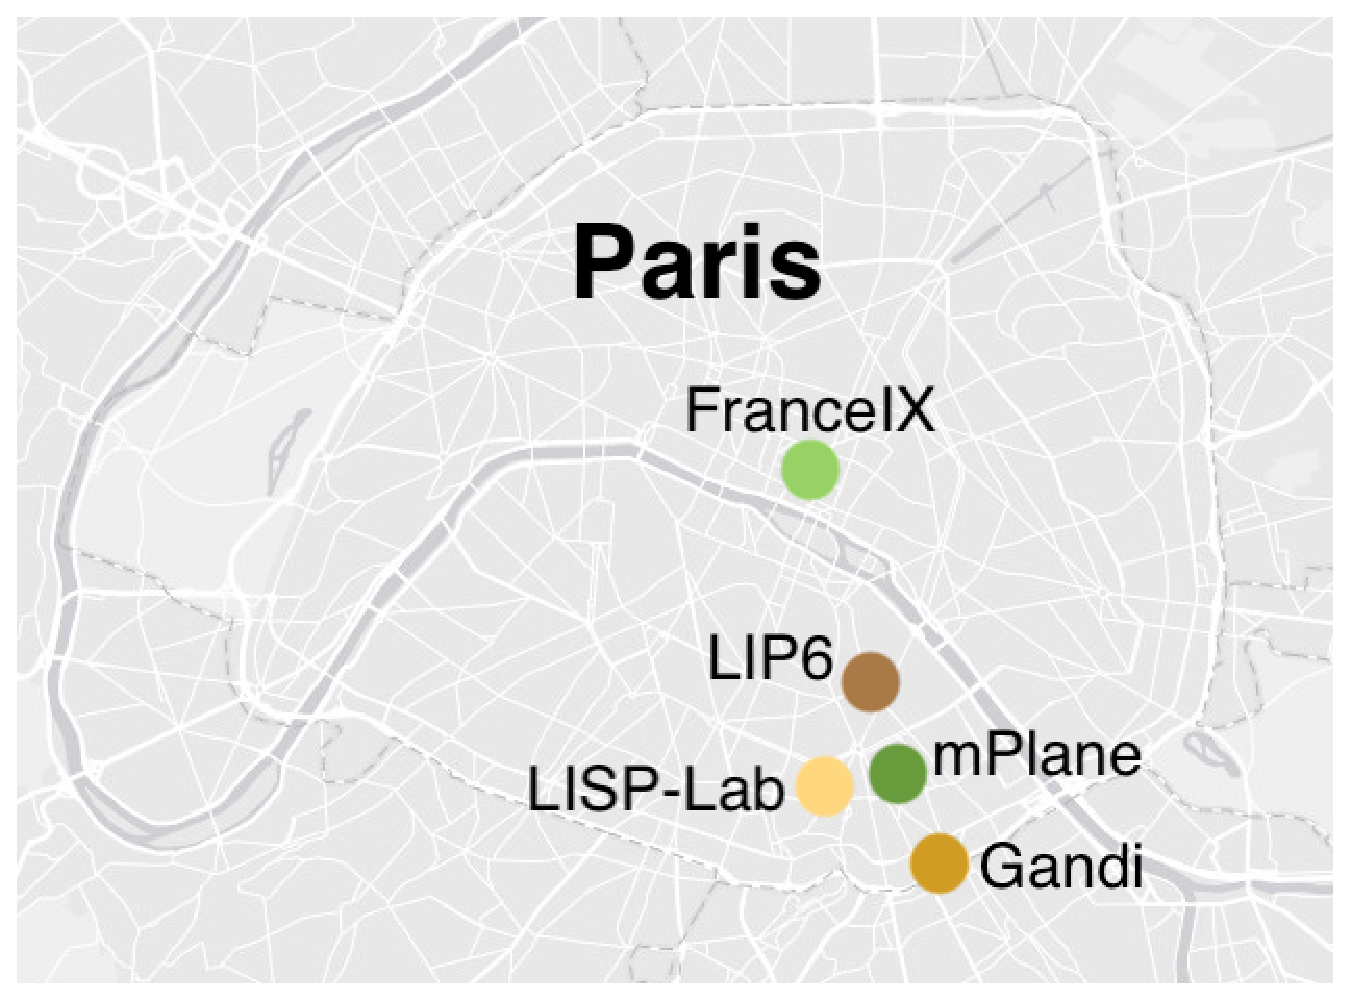
\includegraphics[width=0.6\textwidth]{Pics/Probes_loc.eps}
	\caption{Locations of probes and anchor in 2016}
	\label{Probes_location_2016}
\end{figure}
%-< END FIGURE >--------------------------------------------------------------------

%-< TABLE >-----------------------------------------------------------------
\begin{table}[!tb]
	\centering
	\caption{Location of LISP Beta Network PxTRs in 2016}
	\label{PxTR_loc_2016}{
	\resizebox{0.35\textwidth}{!}{%
		\begin{tabular}{@{}c|c|c@{}}
			\hline\hline
			Number & Continent  & Country   \\ \hline
			1 & Europe & Netherlands     	\\  \hline     
			2 & Europe & Denmark     	\\  \hline
			3 & Europe & Norway     	\\  \hline 
			4 & America & US     	\\  \hline      
			5 & America & US     	\\  \hline         
			6 & Asia & Japan     	\\  \hline  \hline                      
		\end{tabular}
	}}
\end{table}
%-< END TABLE >-----------------------------------------------------------------
% In order to ensure comprehensiveness and accuracy, we need some other probes geographically close to each other having both IPv4 and IPv6 address as comparative items. Ideally, they are connected through both the (non-) academic network provider and (non-) LISP platform. Thus, we selected 4 other probes located in Paris and their locations are shown in Fig.~\ref{Probes_location_2016}. 
The newly added LIP6 probe ($\#2403$) also connects to academic network behind both LISP Beta Network and LISP-Lab platform. When this probe communicates with the hosts in legacy Internet, it uses PETR of LISP-Lab by configuration, while return traffic goes through one of 6 PITRs of LISP Beta Network according to the BGP behavior. Depending on the BGP announcement to the legacy host, a different PITR is used. The more precise location of PITRs on LISP Beta Network is shown in Tab.~\ref{PxTR_loc_2016}: 3 are in Europe (Netherlands, Denmark and Norway), 2 are in US, and 1 is in Asia (Japan). Both LISP probes have a MPLS tunnel from their ITRs to the PETR at Lyon for IPv4, while for IPv6, the ITR of LIP6 probe is configured to use normal BGP routing to reach the PETR in Lyon (i.e., PETR is used but without MPLS VPN). The use of the MPLS tunnel IPv4 packets experience a shorter path compared to the IPv6 BGP-based one. Thus, theoretically the IPv4 packets sending from the LIP6 probe should arrive to PETR faster than those of IPv6. The configuration of two LISP probes are listed in Tab.~\ref{LISP_config}. 

%-< TABLE >-----------------------------------------------------------------
\begin{table}[!tb]
	\centering
	\caption{Configuration of two LISP probes in 2016}
	\label{LISP_config}{
	\resizebox{0.6\textwidth}{!}{%
		\begin{tabular}{@{}c|c|c@{}}
			\hline\hline
			Probe & PETR in Lyon  & PITR   \\ \hline
			LISP-Lab (IPv4) &  Via MPLS Tunnel & Lyon \\ 
			& & (Via MPLS Tunnel) 	\\  \hline      
			LIP6 (IPv4) &  Via MPLS Tunnel & LISP Beta Network     	\\  \hline     
			LISP-Lab (IPv6) &  not used  & Lyon     	\\  \hline     
			LIP6 for (IPv6) &  Via BGP Routing & LISP Beta Network     	\\  \hline \hline               
		\end{tabular}
	}}
\end{table}
%-< END TABLE >-----------------------------------------------------------------

Since the rmd probe is not configured with an IPv6 address, we replace it by the Gandi probe (\#3141), which also resides in an industrial network and also uses the conventional routing for both IPv4 and IPv6. % Although it is a little further to the LISP-Lab probe than the rmd probe, it is the nearest probe having both IPv4 and IPv6. 
As the mPlane probe and the FranceIX anchor satisfy all the requirements of this experiment, we still keep them as the reference. The locations of all the probes and anchor are shown in Fig.~\ref{Probes_location_2016}. Tab.~\ref{Probes_config_2016} shows the different configurations of probes.

%-< TABLE >-----------------------------------------------------------------
\begin{table}[!tb]
	\centering
	\caption{Different configurations of probes in 2016}
	\label{Probes_config_2016}{
	\resizebox{0.6\textwidth}{!}{%
		\begin{tabular}{@{}c|c|c|c@{}}
			\hline\hline
			Name & using LISP & network type  & probe/anchor   \\ \hline
			LISP-Lab &  yes & academic & probe\\  \hline
			LIP6 &  yes & academic & probe     	\\  \hline     
			mPlane &  no  & academic & probe     	\\  \hline     
			Gandi &  no & industrial & probe     	\\  \hline 
			FranceIX &  no & industrial & anchor     	\\  \hline \hline               
		\end{tabular}
	}}
\end{table}
%-< END TABLE >-----------------------------------------------------------------

What we care about is the delay performance and the path of LISP interworking with legacy Internet. Thus, we rely on the ping and traceroute tools provided by RIPE Atlas. As destinations of our measurements, we selected the 500 most popular websites (according to worldwide website ranking provided by Alexa [24]), which reply to IPv4 ping and traceroute. Among them, 122 websites are configured with IPv6 address. Thus, in our experiment, 500 IPv4 and 122 IPv6 addresses are the destinations of ping and traceroute. We develop a Python script to schedule the experiment campaign by using the API provided by RIPE Atlas. The parameters of experiment campaign are as follows: the experiment campaign lasts 15 days (from December 15\textsuperscript{th} to 29\textsuperscript{th} 2016). The 5 chosen probes ping and traceroute to 500 IPv4 and 122 IPv6 addresses. The intervals of ping and traceroute measurements are respectively 30 minutes and 60 minutes. We want to evaluate LISP interworking performance as frequently as possible, but each probe sequentially launches 622 traceroute measurements, which last more than 30 minutes. To avoid the heavy traffic burden and guarantee that all the measurements in a same experimental round can be finished before next round, we set the sampling interval of traceroute at 60 minutes. As a summary, the results presented in this journal come from the following 4 experiment campaigns:
\begin{itemize}[noitemsep,topsep=0pt]
	\item 5 probes ping to 500 destinations during 15 days with an interval of 30 minutes (IPv4).
	\item 5 probes ping to 122 destinations during 15 days with an interval of 30 minutes (IPv6).
	\item 5 probes traceroute to 500 destinations during 15 days with an interval of 60 minutes (IPv4).
	\item 5 probes traceroute to 122 destinations during 15 days with an interval of 60 minutes (IPv6).
\end{itemize}

From the experiment, we find that some websites actually resolve to the same IPv4 (34 over 500) or IPv6 (47 over 122) addresses. Further, for some destinations, at least one probe (mainly the LIP6 probe) does not get any responses of \emph{ping} during the whole experiment (42 for IPv4 and 10 for IPv6). In this paper, we filtered the anycast destinations and only consider responding destinations. Thus, after cleaning the traces for the above reasons, all the results of \emph{ping} measurements used in the following subsections consists on the 5 chosen probes as the experimental sources and 424 IPv4 and 65 IPv6 responding addresses as the destinations. Differently from the ping measurements, for the \emph{traceroute} dataset, all the successful \emph{traceroute} responses from each probe are kept for further analysis.


 %-< SECTION >--------------------------------------------------------------------
\section{IPv4 Ping results from Dataset 2015}
\label{sec:pxtr_ping_v4_2015}
% \begin{itemize}[noitemsep,topsep=0pt]
%     \item CDF of average RTT between different probes
%     \item Correlation coefficient to FranceIX
%     \item Smallest mean and median RTT grouped by continent
%     \item Relative mean and median RTT clustered by continent
% \end{itemize}
%-< FIGURE >--------------------------------------------------------------------
    \begin{figure}[!t]
     	\centering
     	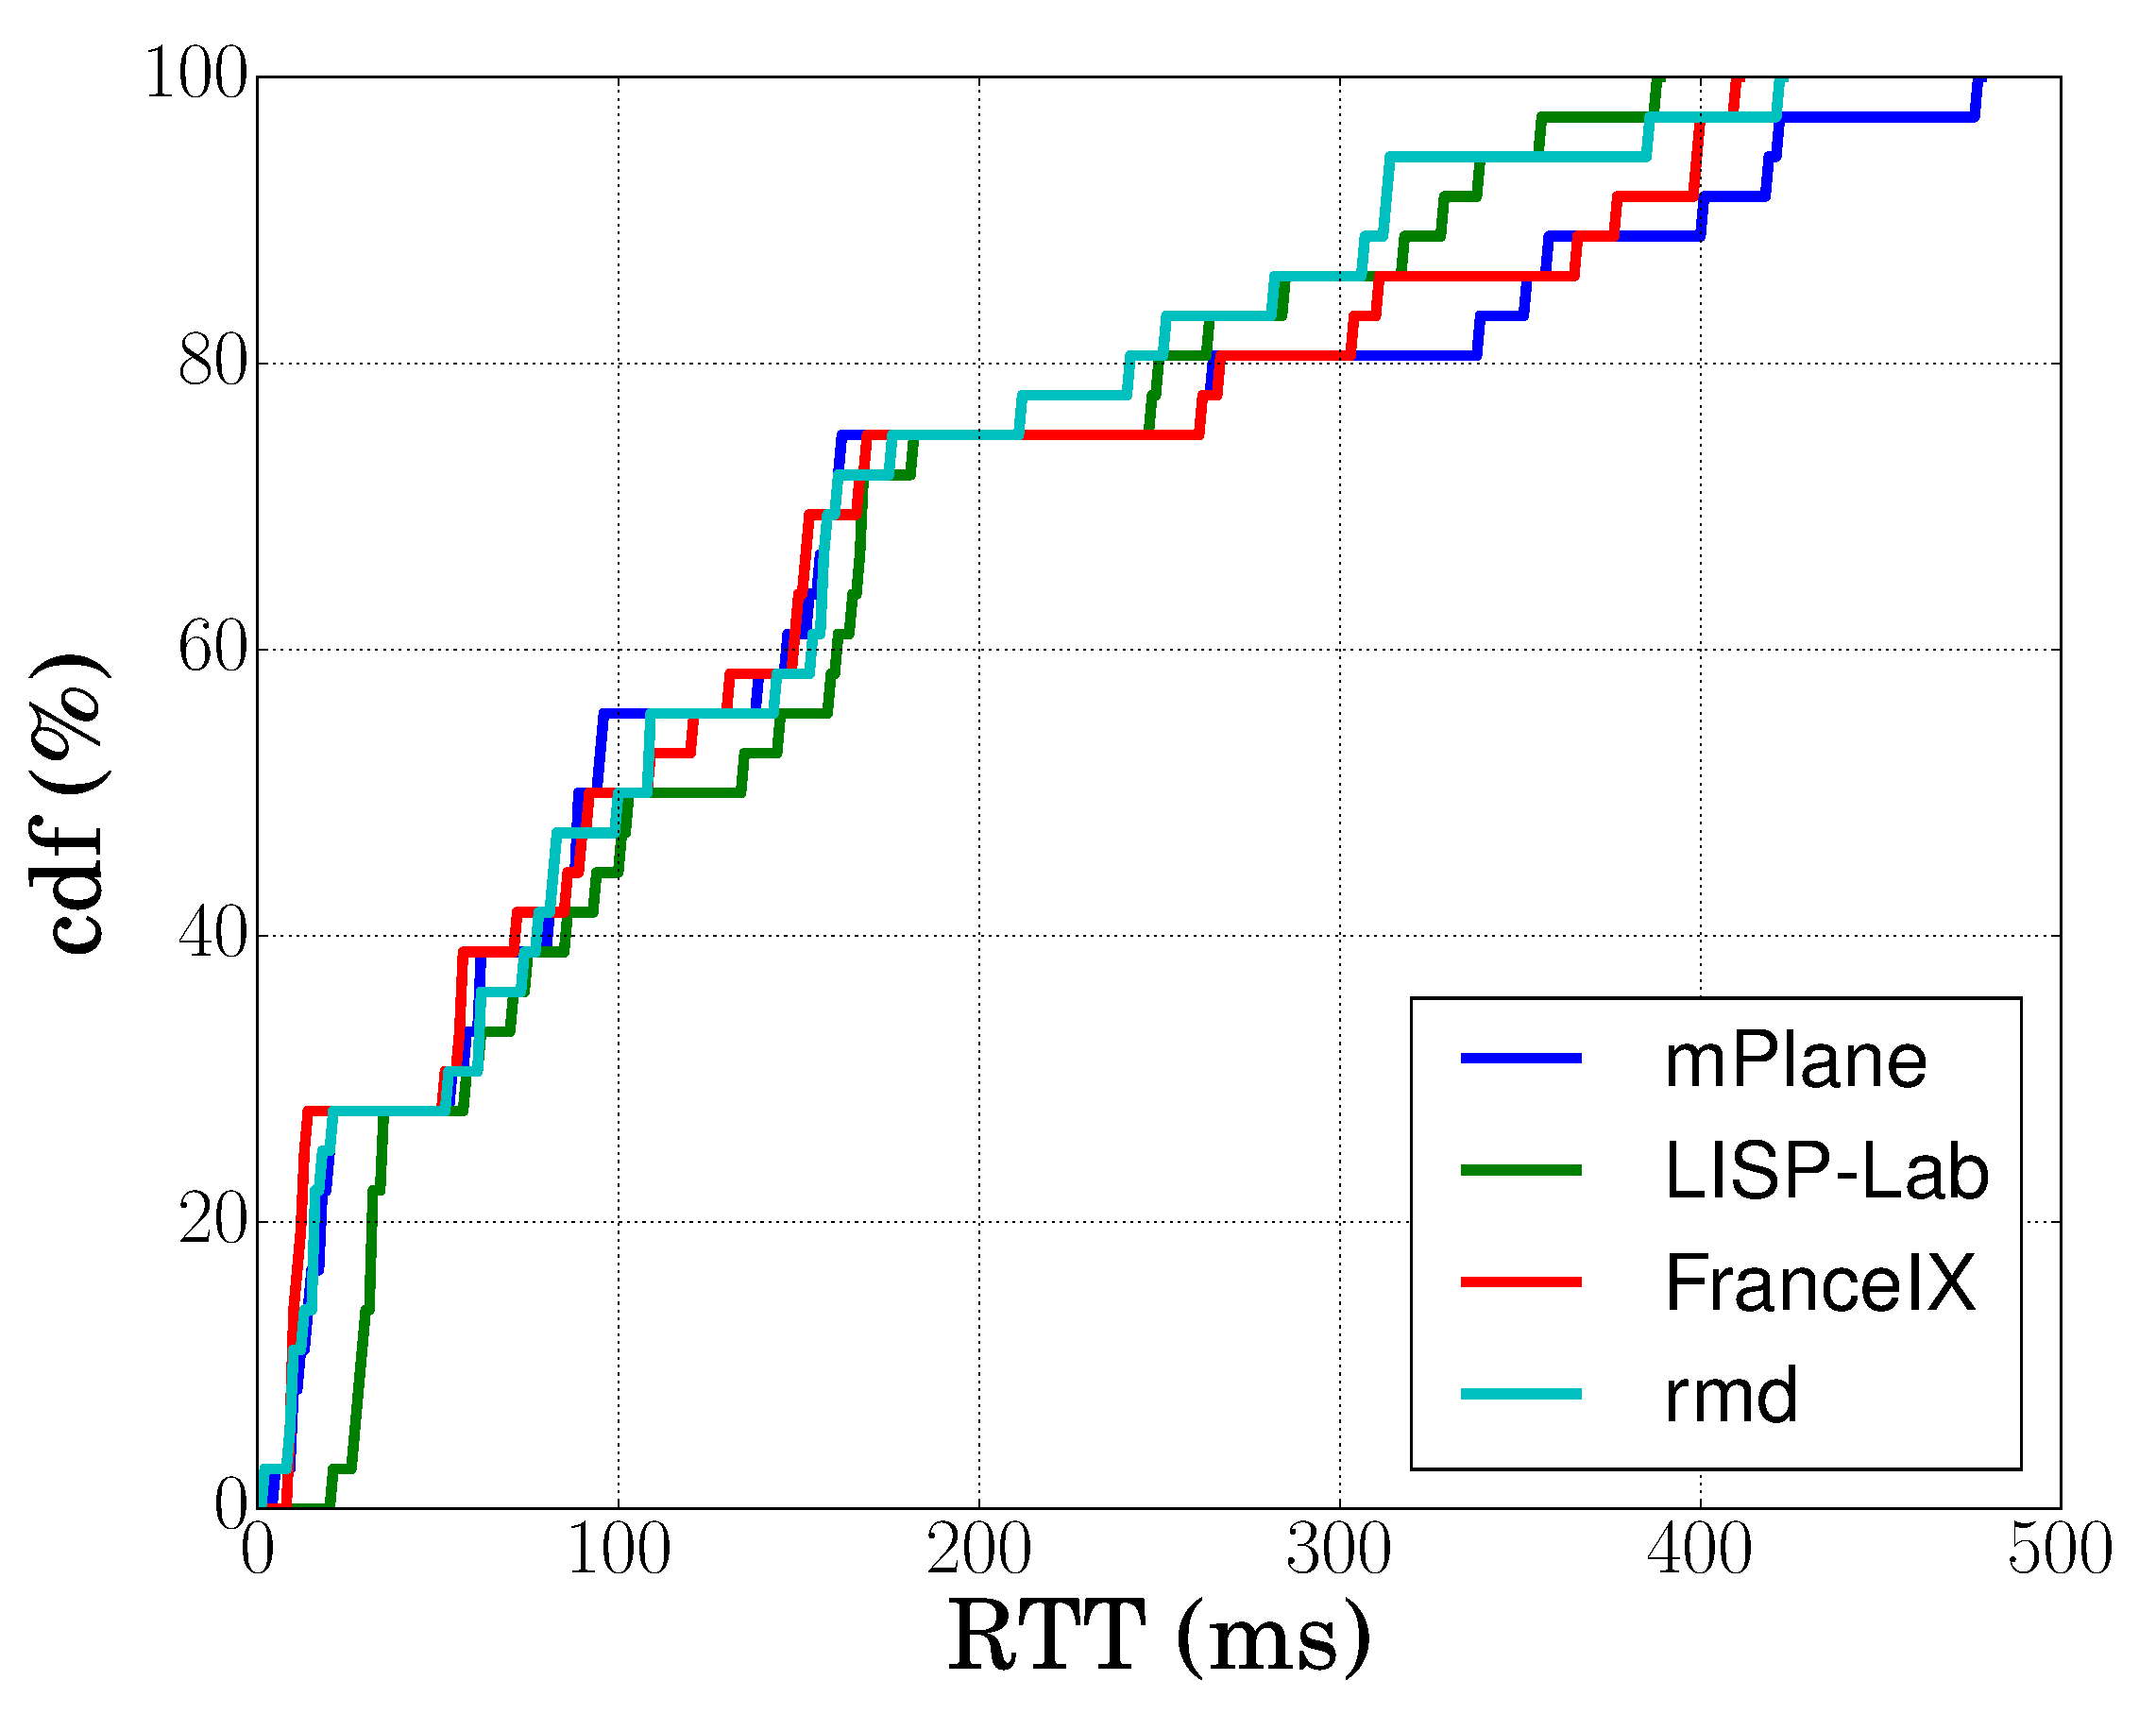
\includegraphics[width=0.6\textwidth]{Pics/2015/CDF_RTT_avg.eps}
     	\caption{CDF of average RTT between different probes from Dataset 2015}
     	\label{CDF_RTT_avg_v4_2015}
     \end{figure}
    %-< END FIGURE >-----------------------------------------------------------------
    
Fig.~\ref{CDF_RTT_avg_v4_2015} shows the cumulative distribution function (CDF) of average RTTs towards the selected 50 targets. Since the experimental destinations are located all over the world, the range of observed RTTs varies from few milliseconds (ms) to nearly five hundreds ms. When the RTT values are in the small range, especially when RTT is less than 50 ms, the latency from LISP-Lab probe is always higher than the three others and the difference is mainly around 10 ms. This latency difference is caused by the stretch introduced by the proxy technology (cf. Sec.\ref{sec:background_Interworking}), since every packet sent between LISP-Lab probe and the legacy Internet has to pass through the LISP-Lab PxTR, which is located in Lyon (approximately $400km$ away from the probe). As the RTT increases, actually the difference (surprisingly) decreases. When the RTT around 200 ms is reached, all probes show basically the same RTT. Around such RTT values, the destinations concentrate in North America. Going further in the high range RTT values, i.e., more than 350 ms, when destinations are mainly located in Asia, the probe in the LISP-Lab domain actually shows the lowest RTT. Thus, it indicates that the network connection between the LISP-Lab PxTR to the (asian) intercontinental destinations has a better performance and the stretch delay from LISP-Lab probe to PxTR can be ignored. We wanted to use traceroute to further investigate the reasons, but it cannot be natively used at that moment, since the LISP-encapsulation prevents its correct function. We explored a new way to find out what happens for Dataset 2016, which is described in Sec.~\ref{sec:pxtr_traceroute}. 
    
We tried to quantify the percentage of times that one probe's RTT is the smallest compared to three others, since the destinations that the different probes contact to are exactly the same. The result shows that in $52.8\%$ of the time, FranceIX shows the smallest RTT to reach the destinations. It is normal that its RTTs are the smallest, since FranceIX is an Internet Exchange Point (IXP), hence well connected, and also acts as one of the anchors of RIPE Atlas, thus with a more powerful hardware. While, only in the $5.6\%$ of the cases, the LISP-Lab probe has the smallest RTT. In this small percentage the main contribution comes from Intercontinental destinations, i.e., when the RTT values belong to high range.
    
\begin{figure}[!t]
	\begin{minipage}[c]{.49\linewidth}
		\begin{center}
			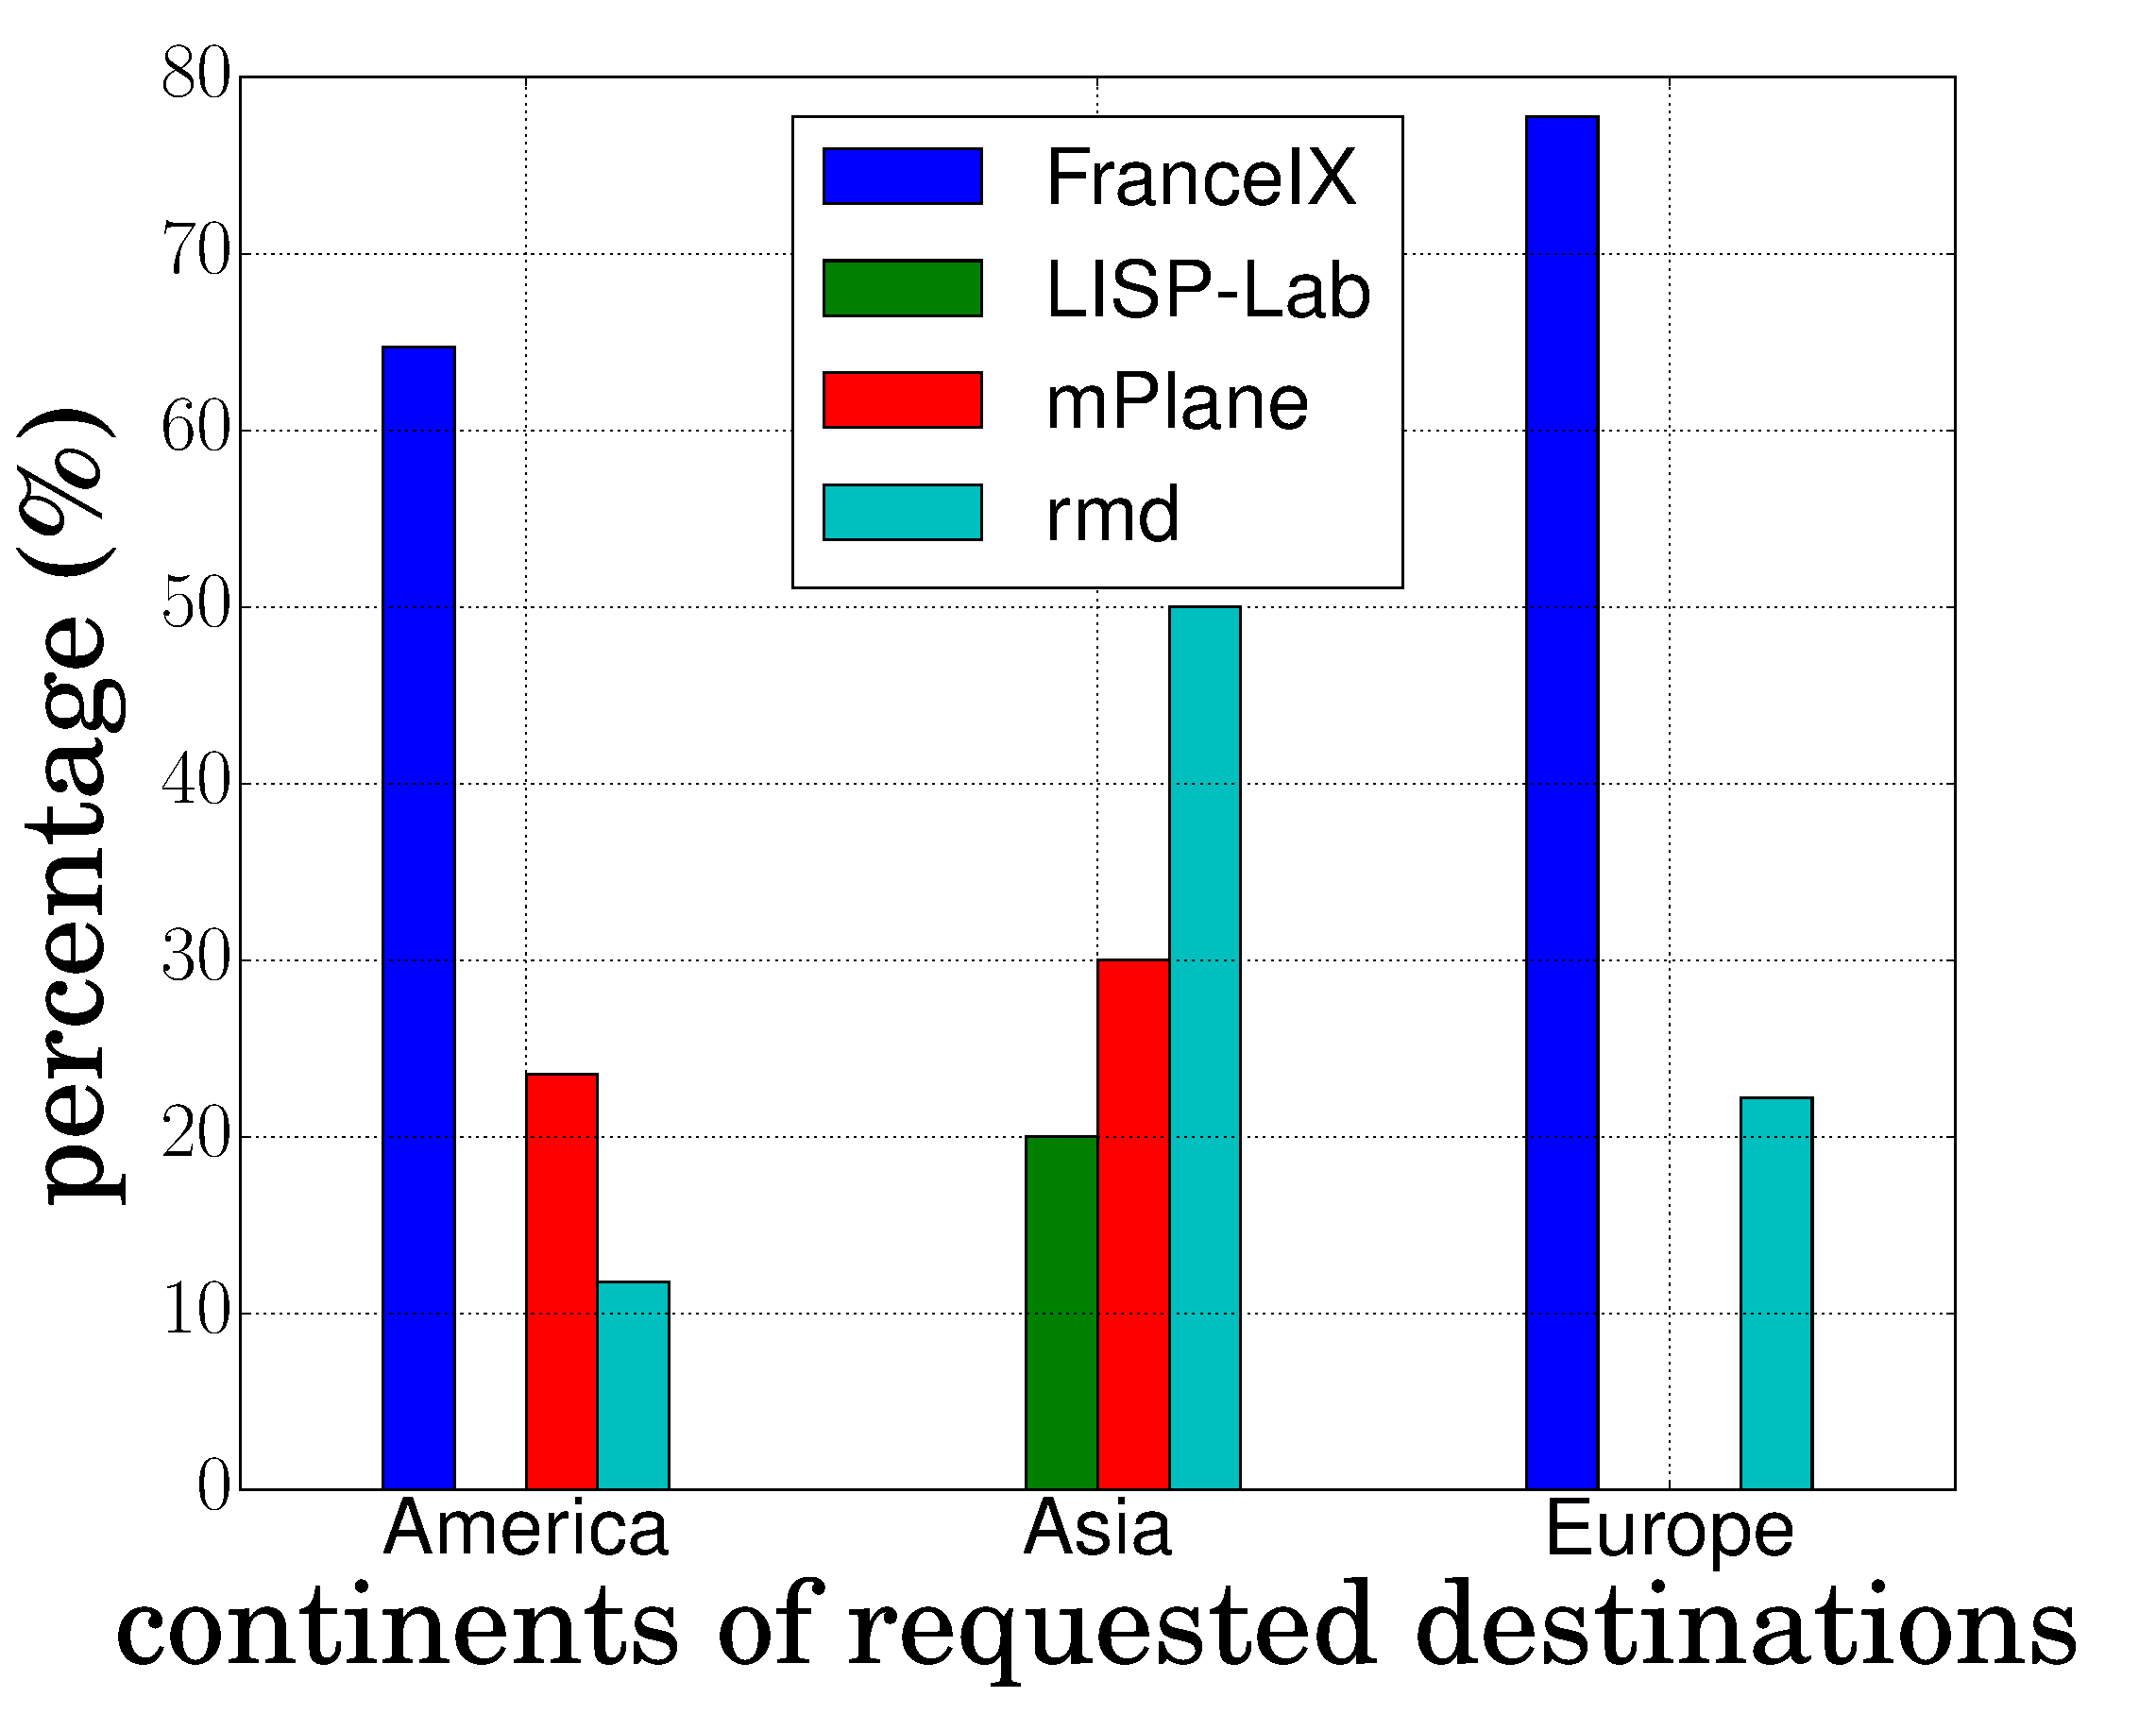
\includegraphics[width=.9\linewidth]{Pics/2015/4_probes_to_alexa_top50_proportion_mean_bar_geo.eps}
		\end{center}
	\end{minipage}
	\begin{minipage}[c]{.49\linewidth}
		\begin{center}
			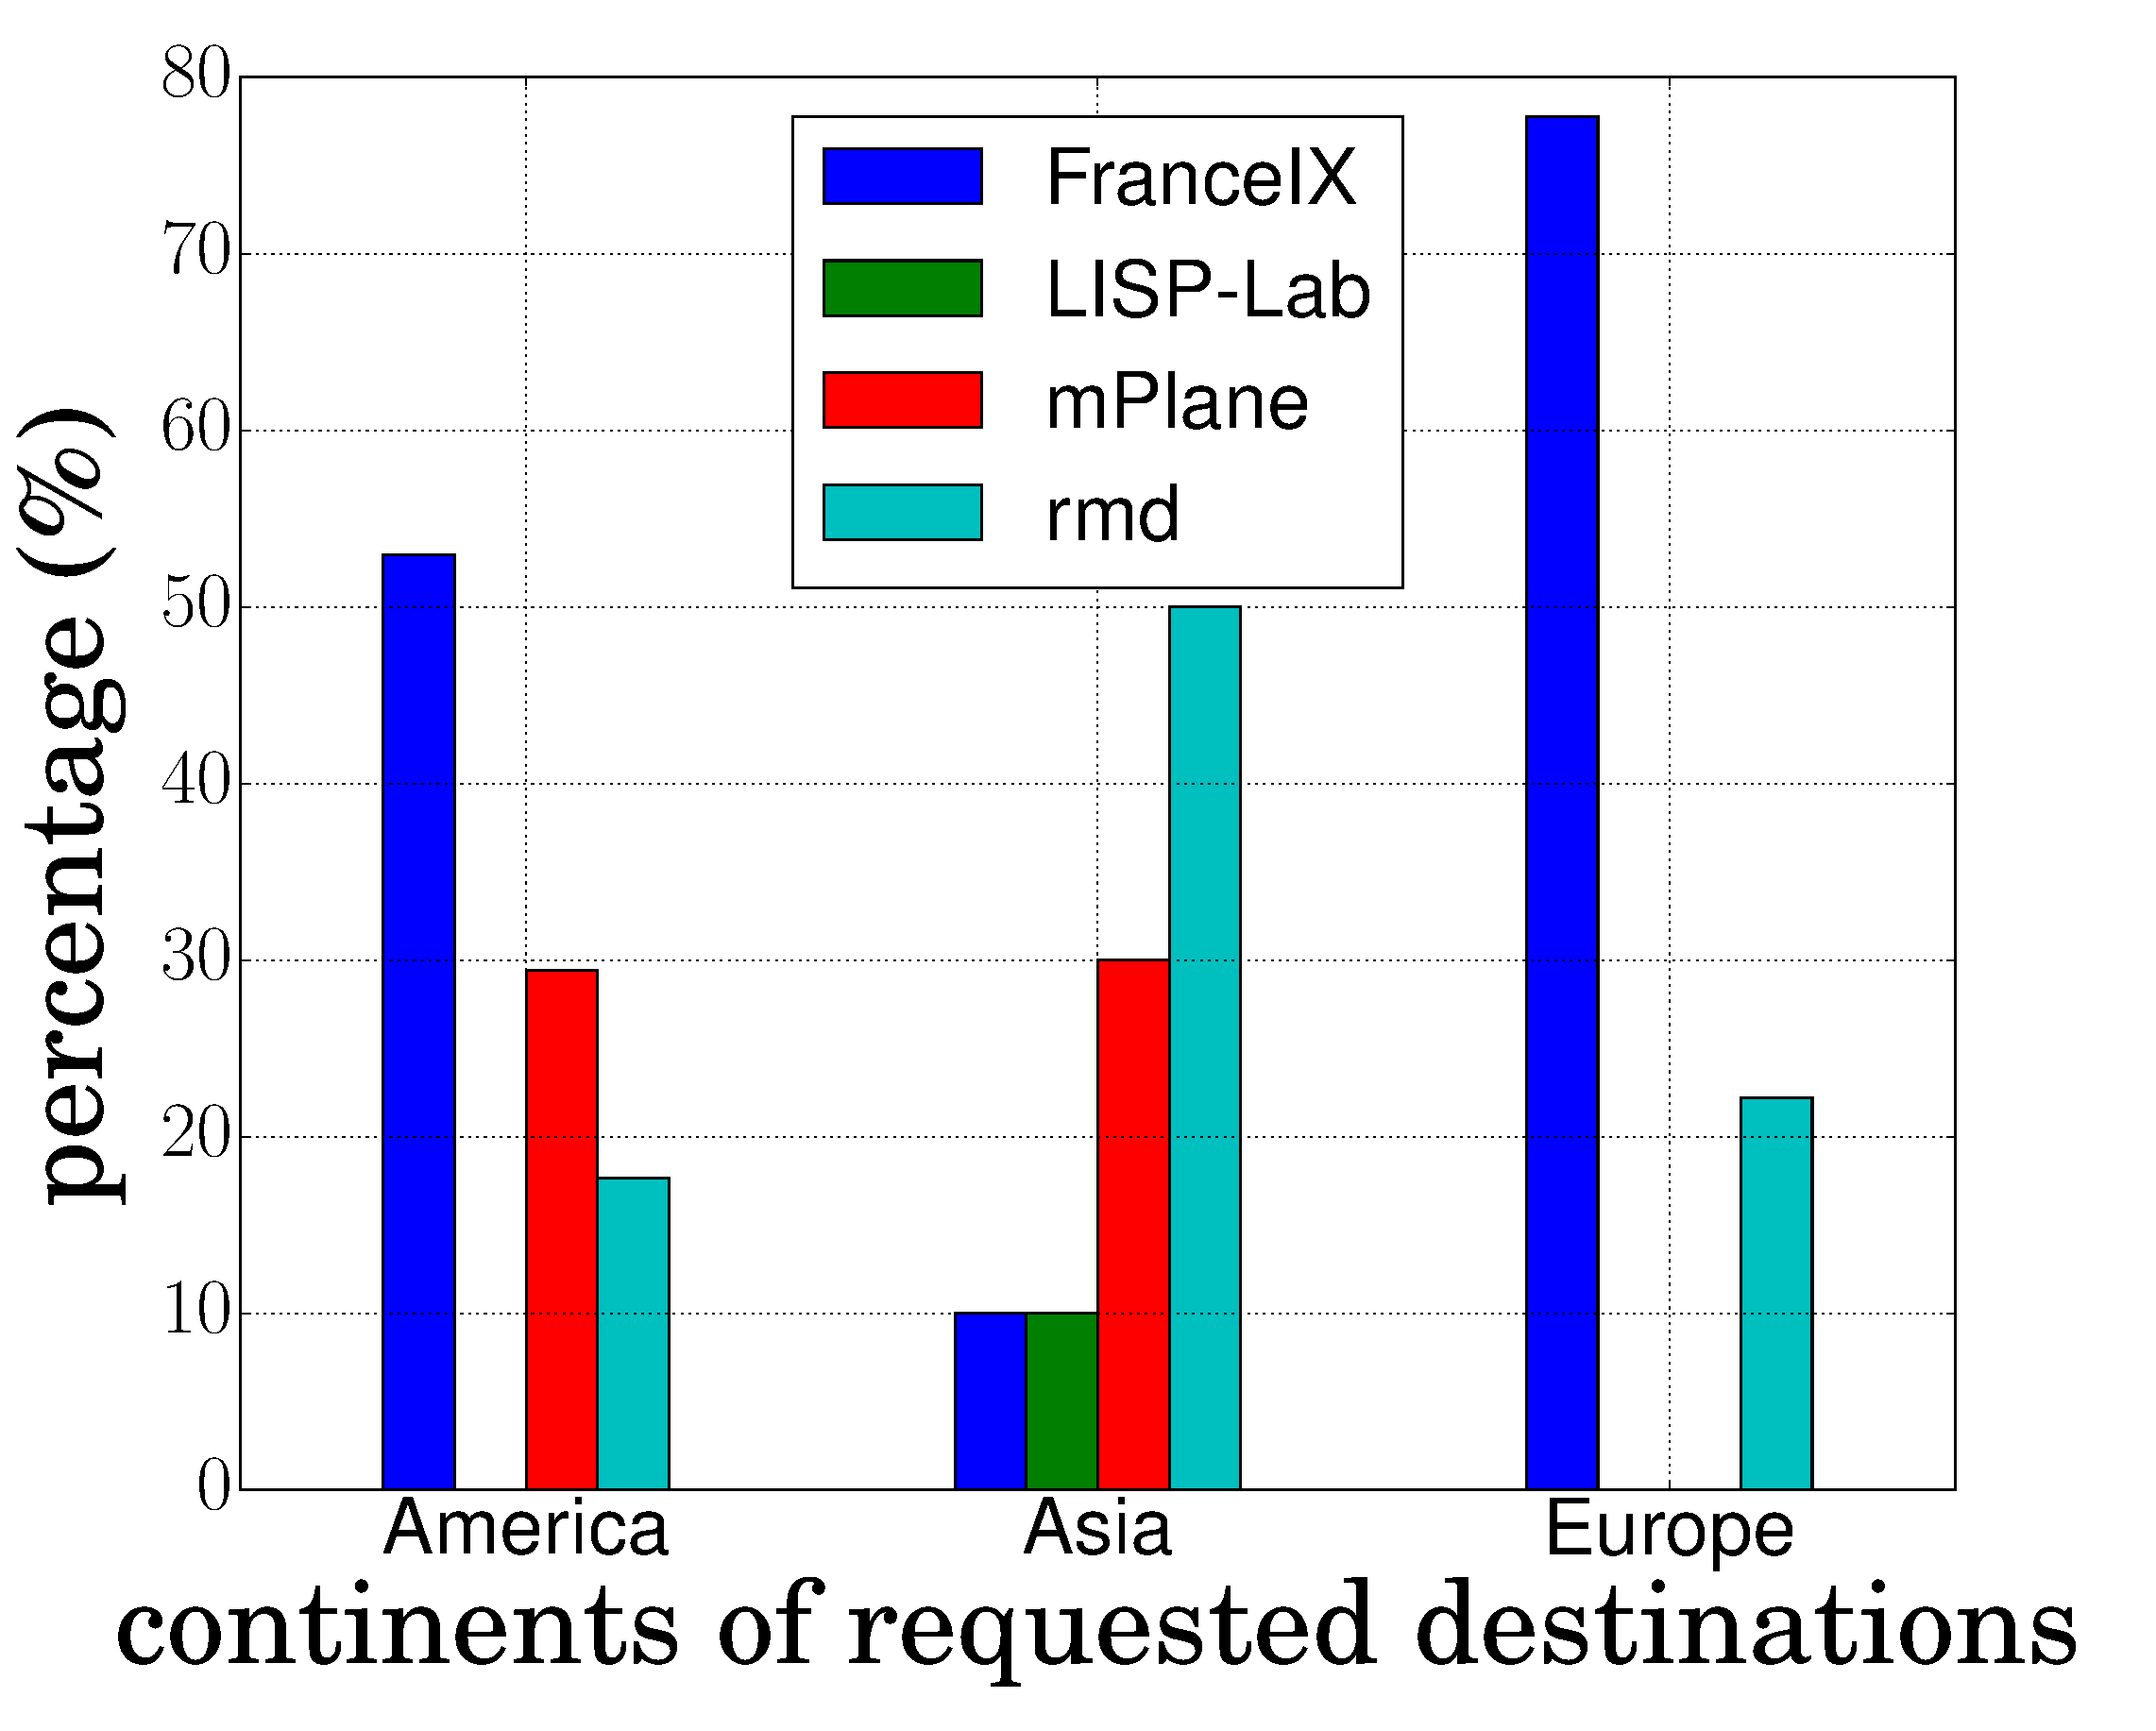
\includegraphics[width=.9\linewidth]{Pics/2015/4_probes_to_alexa_top50_proportion_median_bar_geo.eps}
		\end{center}
	\end{minipage}
	\caption{Smallest mean RTT (left) and smallest median RTT (right) grouped by continent from Dataset 2015.}
	\label{4_probes_to_alexa_top50_proportion_bar_geo}
\end{figure}
	
Fig.~\ref{4_probes_to_alexa_top50_proportion_bar_geo} depicts the percentage of times that one probe's RTT is the smallest compared to three other probes grouped by continents where the selected targets are located. When the destinations are in Europe and America, FranceIX is the fastest most of the time. % This is reasonable, since FranceIX is an Internet Exchange Point (IXP), acting as Atlas' anchor, thus it is well connected with a more powerful hardware. 
Whereas, the percentage of LISP-Lab is always 0. Its higher RTT is caused by the proxy stretch. %, since traffic between LISP-Lab probe and the legacy Internet has to pass through the LISP-Lab PxTR, which is in Lyon (approx. $400km$ away from the probe). 
When the targets are in Asia, LISP-Lab becomes the fastest with a percentage of $20\%$ (mean RTT) and $10\%$ (median RTT). It indicates that such connection from the LISP-Lab PxTR is faster, so that the stretch can be ignored. The performance of FranceIX is not very stable to the Asian destinations, being the fastest $0\%$ in average, but it is $10\%$ looking at
the median RTT. It shows that FranceIX sometimes has extremely high RTT values to Asian destinations. 
	
\begin{figure}[!t]
	\begin{minipage}[c]{.49\linewidth}
		\begin{center}
			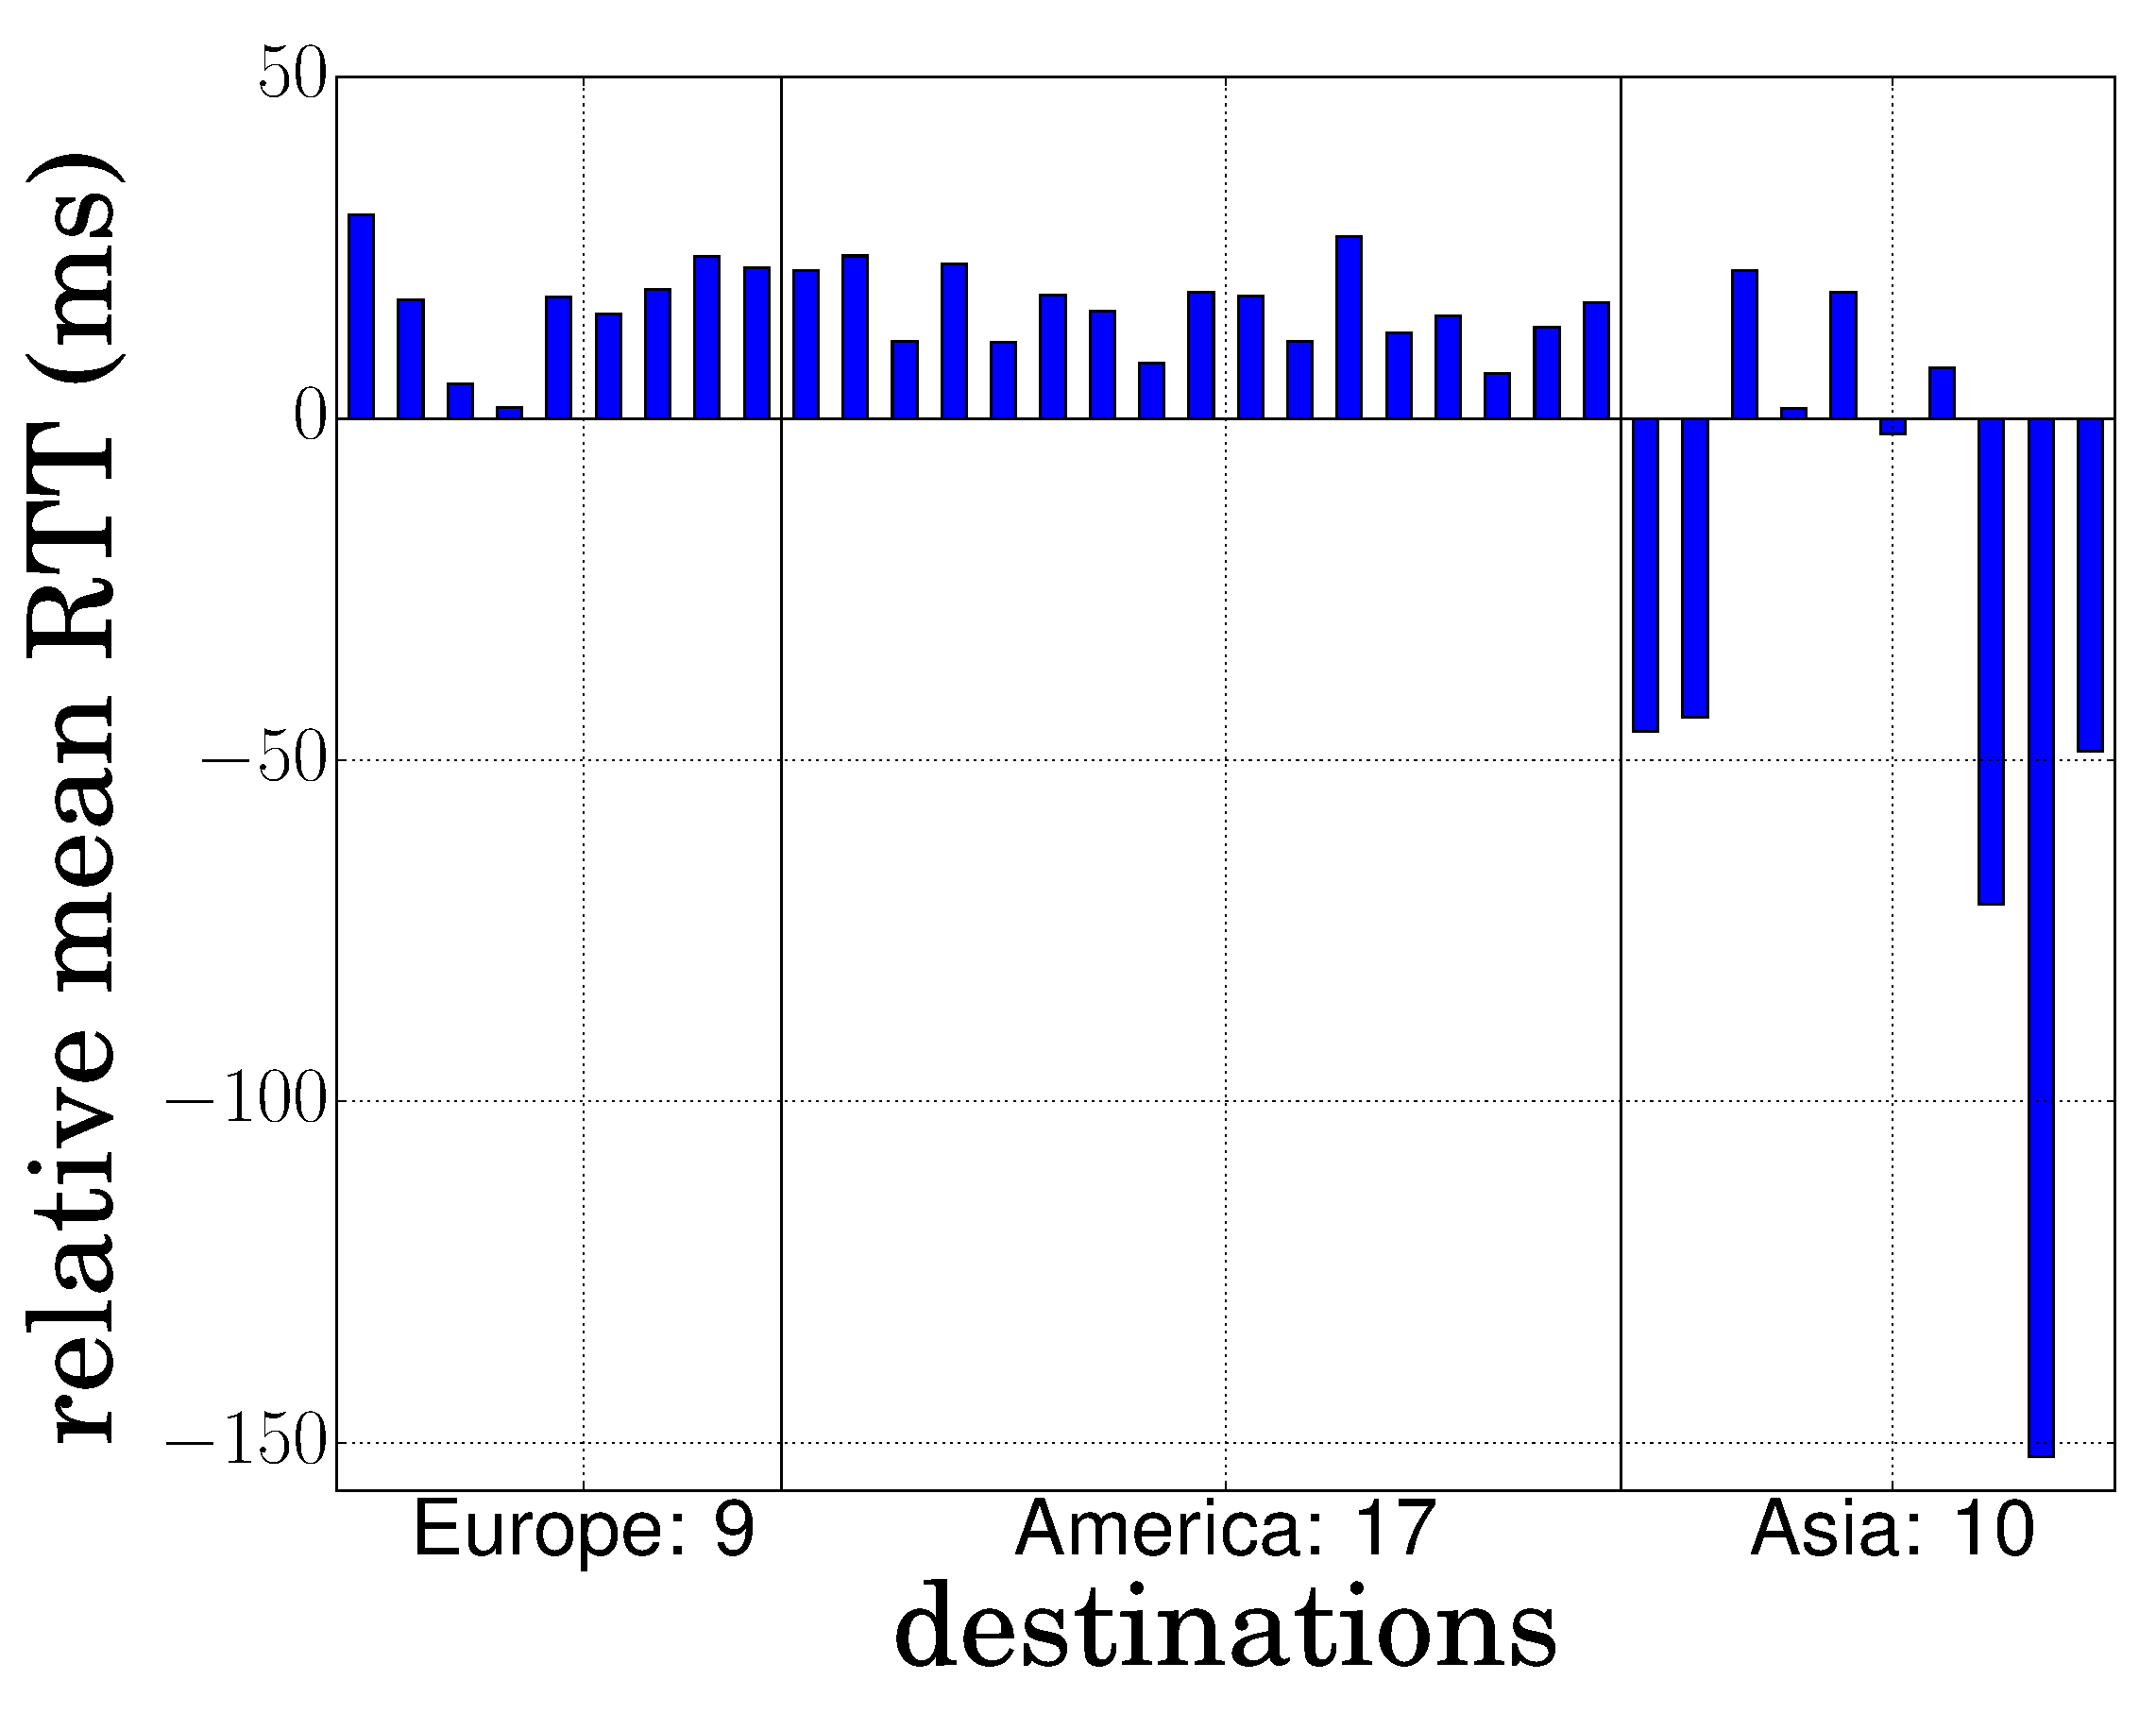
\includegraphics[width=.9\linewidth]{Pics/2015/4_probes_to_alexa_top50_diff_rtt_LISP-Lab_FranceIX_mean_geo.eps}
		\end{center}
	\end{minipage}
	\begin{minipage}[c]{.49\linewidth}
		\begin{center}
			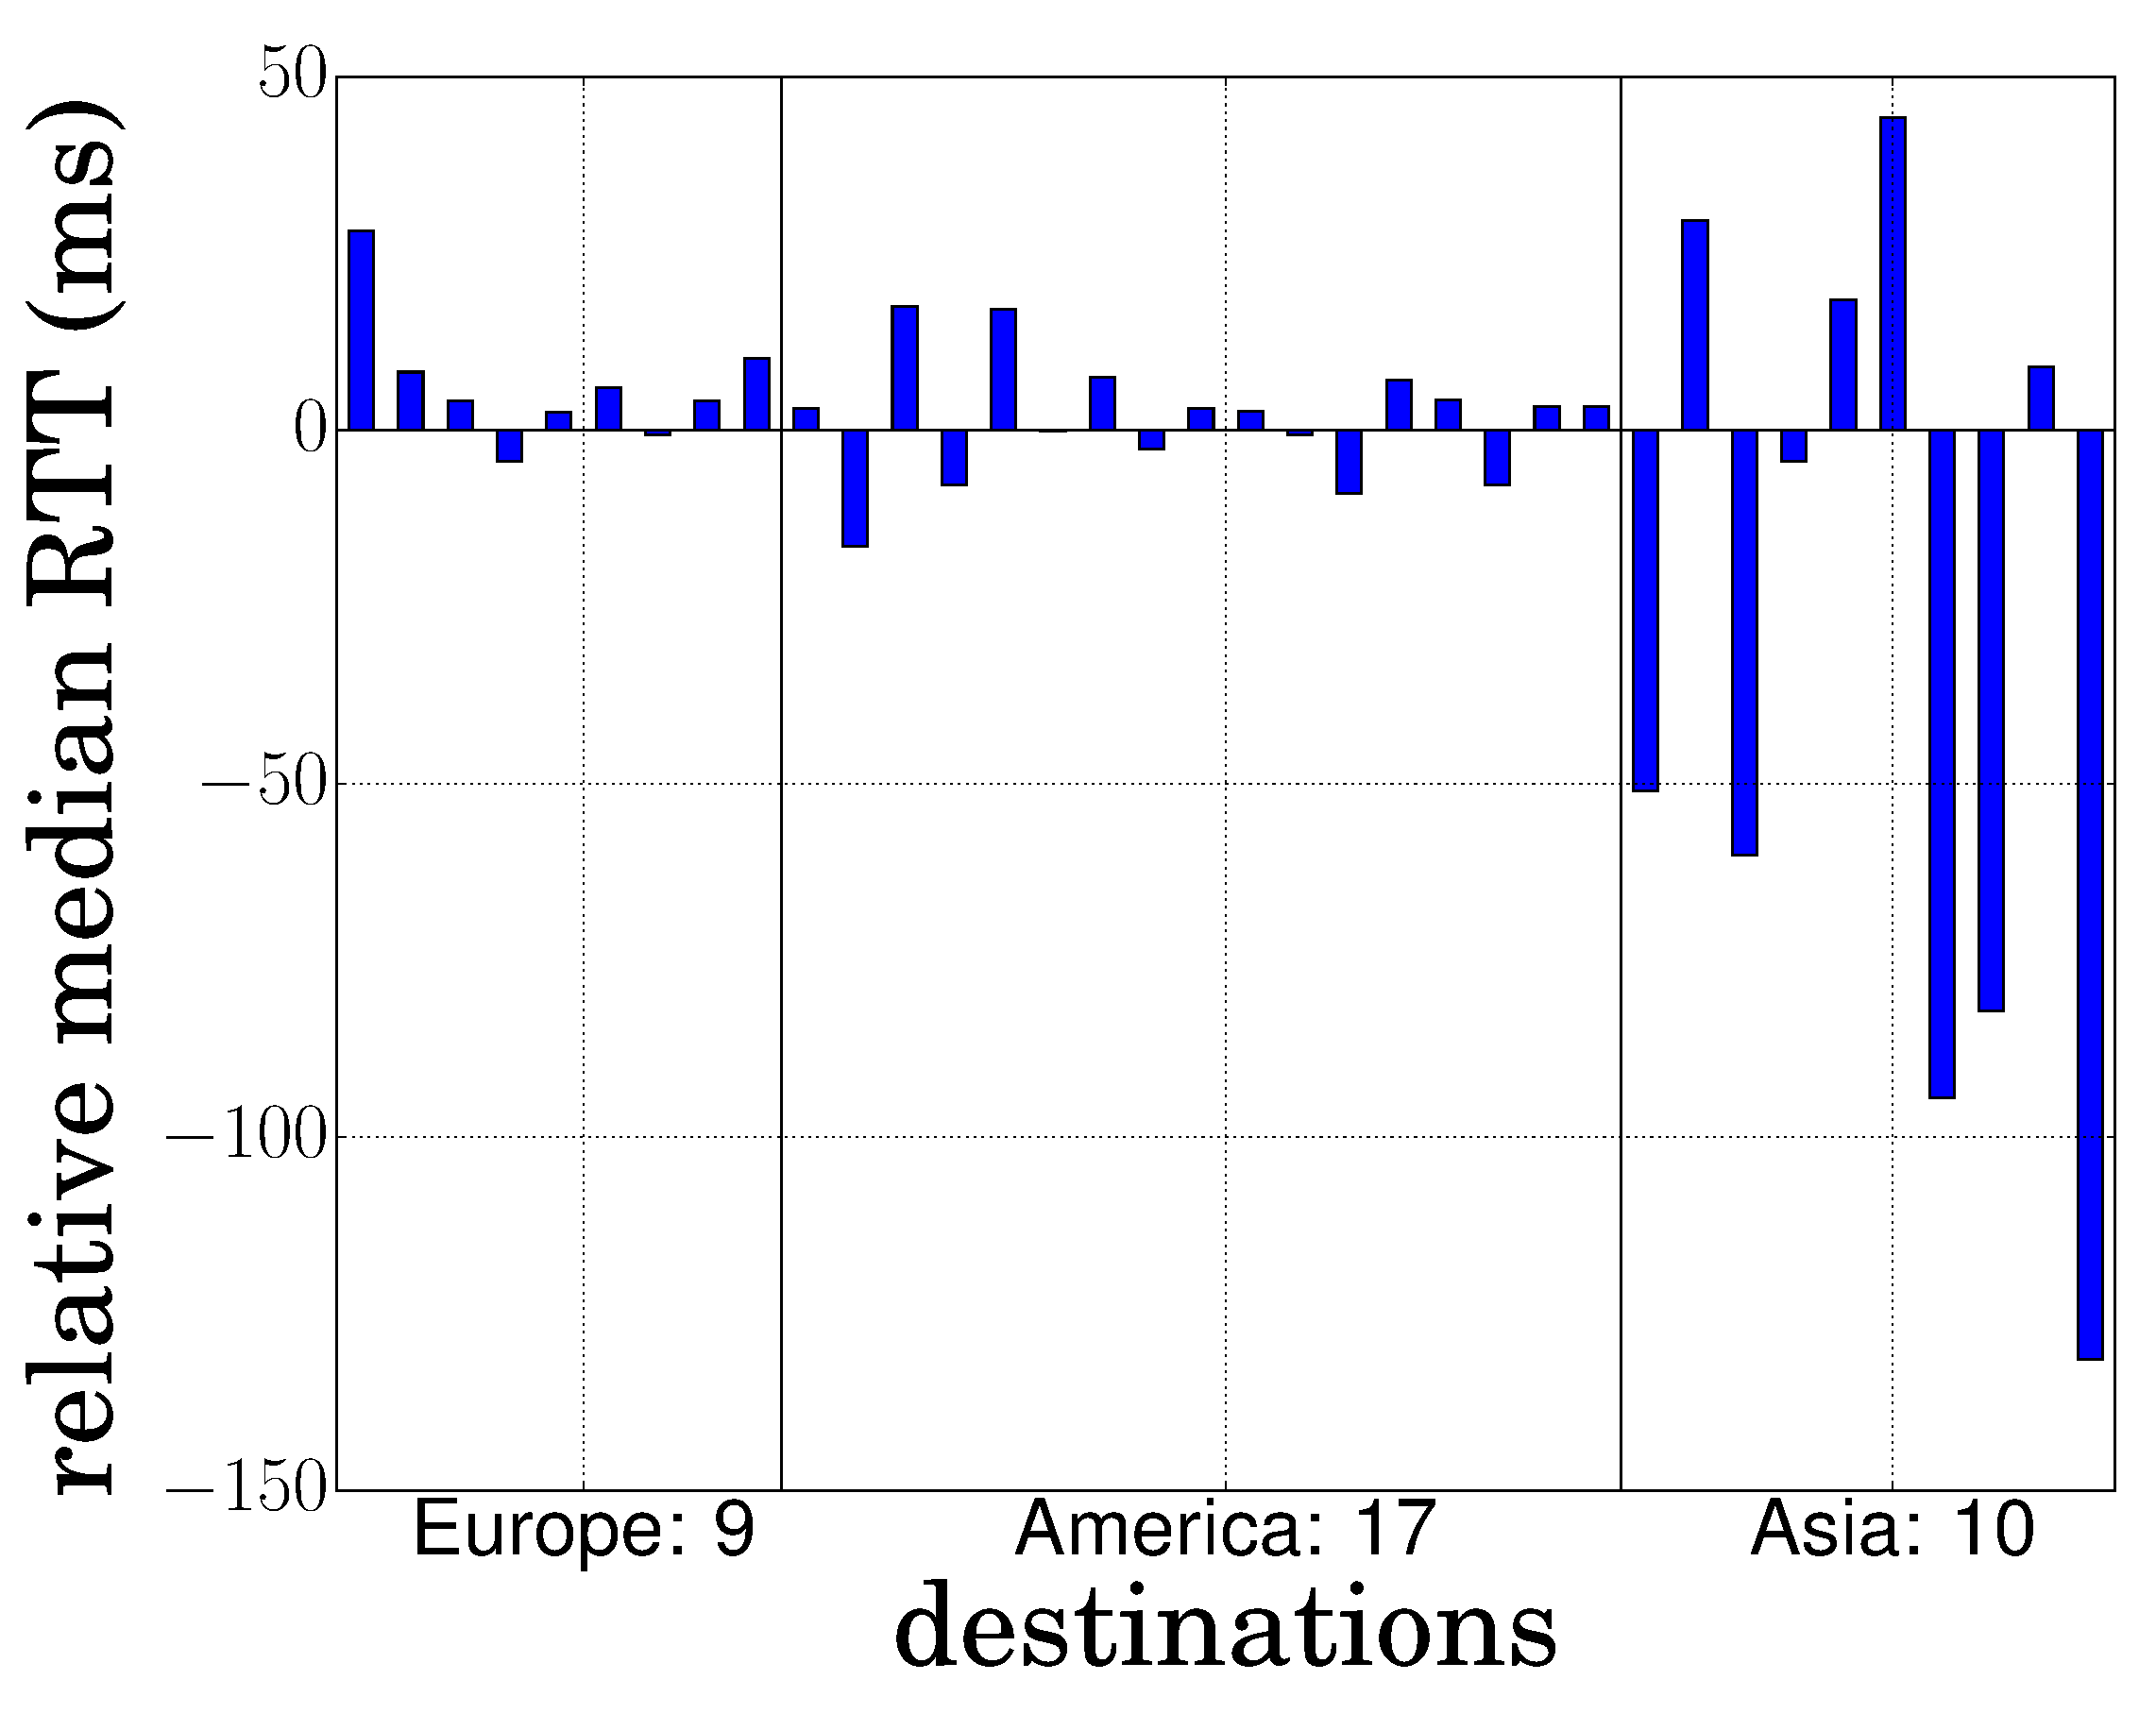
\includegraphics[width=.9\linewidth]{Pics/2015/4_probes_to_alexa_top50_diff_rtt_LISP-Lab_FranceIX_median_geo.eps}
		\end{center}
	\end{minipage}
	\vspace{-0.5mm}
	\caption{Relative mean (left) and median (right) RTT clustered by different continents from Dataset 2015.}
	\label{4_probes_to_alexa_top50_diff_rtt_LISP-Lab_FranceIX_geo}
\end{figure}
	
We also evaluate whether the performance of LISP-Lab is as stable as FranceIX. % We define the relative performance for each destination as: $RTT_{LISP-Lab}$ - $RTT_{FranceIX}$, and the results clustered by continents are shown in Fig.~\ref{4_probes_to_alexa_top50_diff_rtt_LISP-Lab_FranceIX_geo}. 
We define a metric called \emph{Relative RTT (rRTT)} for each destination as: 
\begin{equation} 
    \label{rRTT_ll_2015}
    rRTT_{LL}(d)=RTT_{LL}(d) - RTT_{F}(d)
\end{equation}
where $d$ is the destination, subscriptions $LL$ and $F$ respectively refers to LISP-Lab and FranceIX. The results clustered by continents are shown in Fig.~\ref{4_probes_to_alexa_top50_diff_rtt_LISP-Lab_FranceIX_geo}. The left hand one shows the mean RTT, while the right hand one shows the median RTT. For the European and American targets, LISP-Lab is a little slower than FranceIX but with a stable behavior. On the contrary, for half of the Asian destinations, LISP-Lab is significantly faster than FranceIX. It shows that the network connection between LISP-Lab PxTR and Asian destinations has better performance. Comparing the two subfigures, there is no negative values at all in Europe and America area in left hand figure, but there are some in the right hand one. It indicates that LISP-Lab RTTs to these destinations are very unstable and the variance is quite high.

%-< TABLE >-----------------------------------------------------------------
\begin{table}[!tb]
	\centering
	\caption{Correlation coefficient to FranceIX from Dataset 2015}
	\label{correlation_v4_2015}{
		\resizebox{0.55\textwidth}{!}{%
		\begin{tabular}{@{}c|c|c|c|c@{}}
			\hline\hline
			& LISP-Lab  & mPlane &  rmd &  FranceIX \\ \hline
			Coefficient & 0.9733  & 0.9784 &  0.9646  &  1.0     	\\  \hline\hline                 
		\end{tabular}
	}}
\end{table}
%-< END TABLE >-----------------------------------------------------------------

Since FranceIX shows the best RTT most of the time, we tried to evaluate the correlation between the RTT of the other 3 probes and FranceIX. The purpose is to see if RTT measurements are correlated or totally independent. We compute the correlation coefficient for every RTT series of different probes to all destinations with the ones of FranceIX. Tab.\ref{correlation_v4_2015} shows the results. The absolute value of coefficient is 1 in the case of a perfect direct linear relationship, whereas 0 in the case of no correlation at all. The correlation coefficient of LISP-Lab is 0.9733 (> 0.8), showing a very high correlation with FranceIX, like the other 2 probes. This means that LISP while certainly introducing some overhead, has quite stable performance that does not deviate from normal network operation.


%-< SECTION >--------------------------------------------------------------------
\section{IPv4 Ping results from Dataset 2016}
\label{sec:pxtr_ping_v4_2016}
% \begin{itemize}[noitemsep,topsep=0pt]
%     \item CDF of median RTT between different probes
%     \item Smallest median RTT grouped by continent
%     \item Correlation coefficient to FranceIX
%     \item Relative median RTT clustered by continent for LISP-Lab and LIP6
%     \item Reliability of each probe
%     \item The periodicity check
% \end{itemize}

% With the collected dataset from IPv4 ping experiment, we assess the performance of LISP interworking with legacy Internet in terms of round-trip time (RTT).

%-< FIGURE >--------------------------------------------------------------------
\begin{figure}[!t]
	\centering
	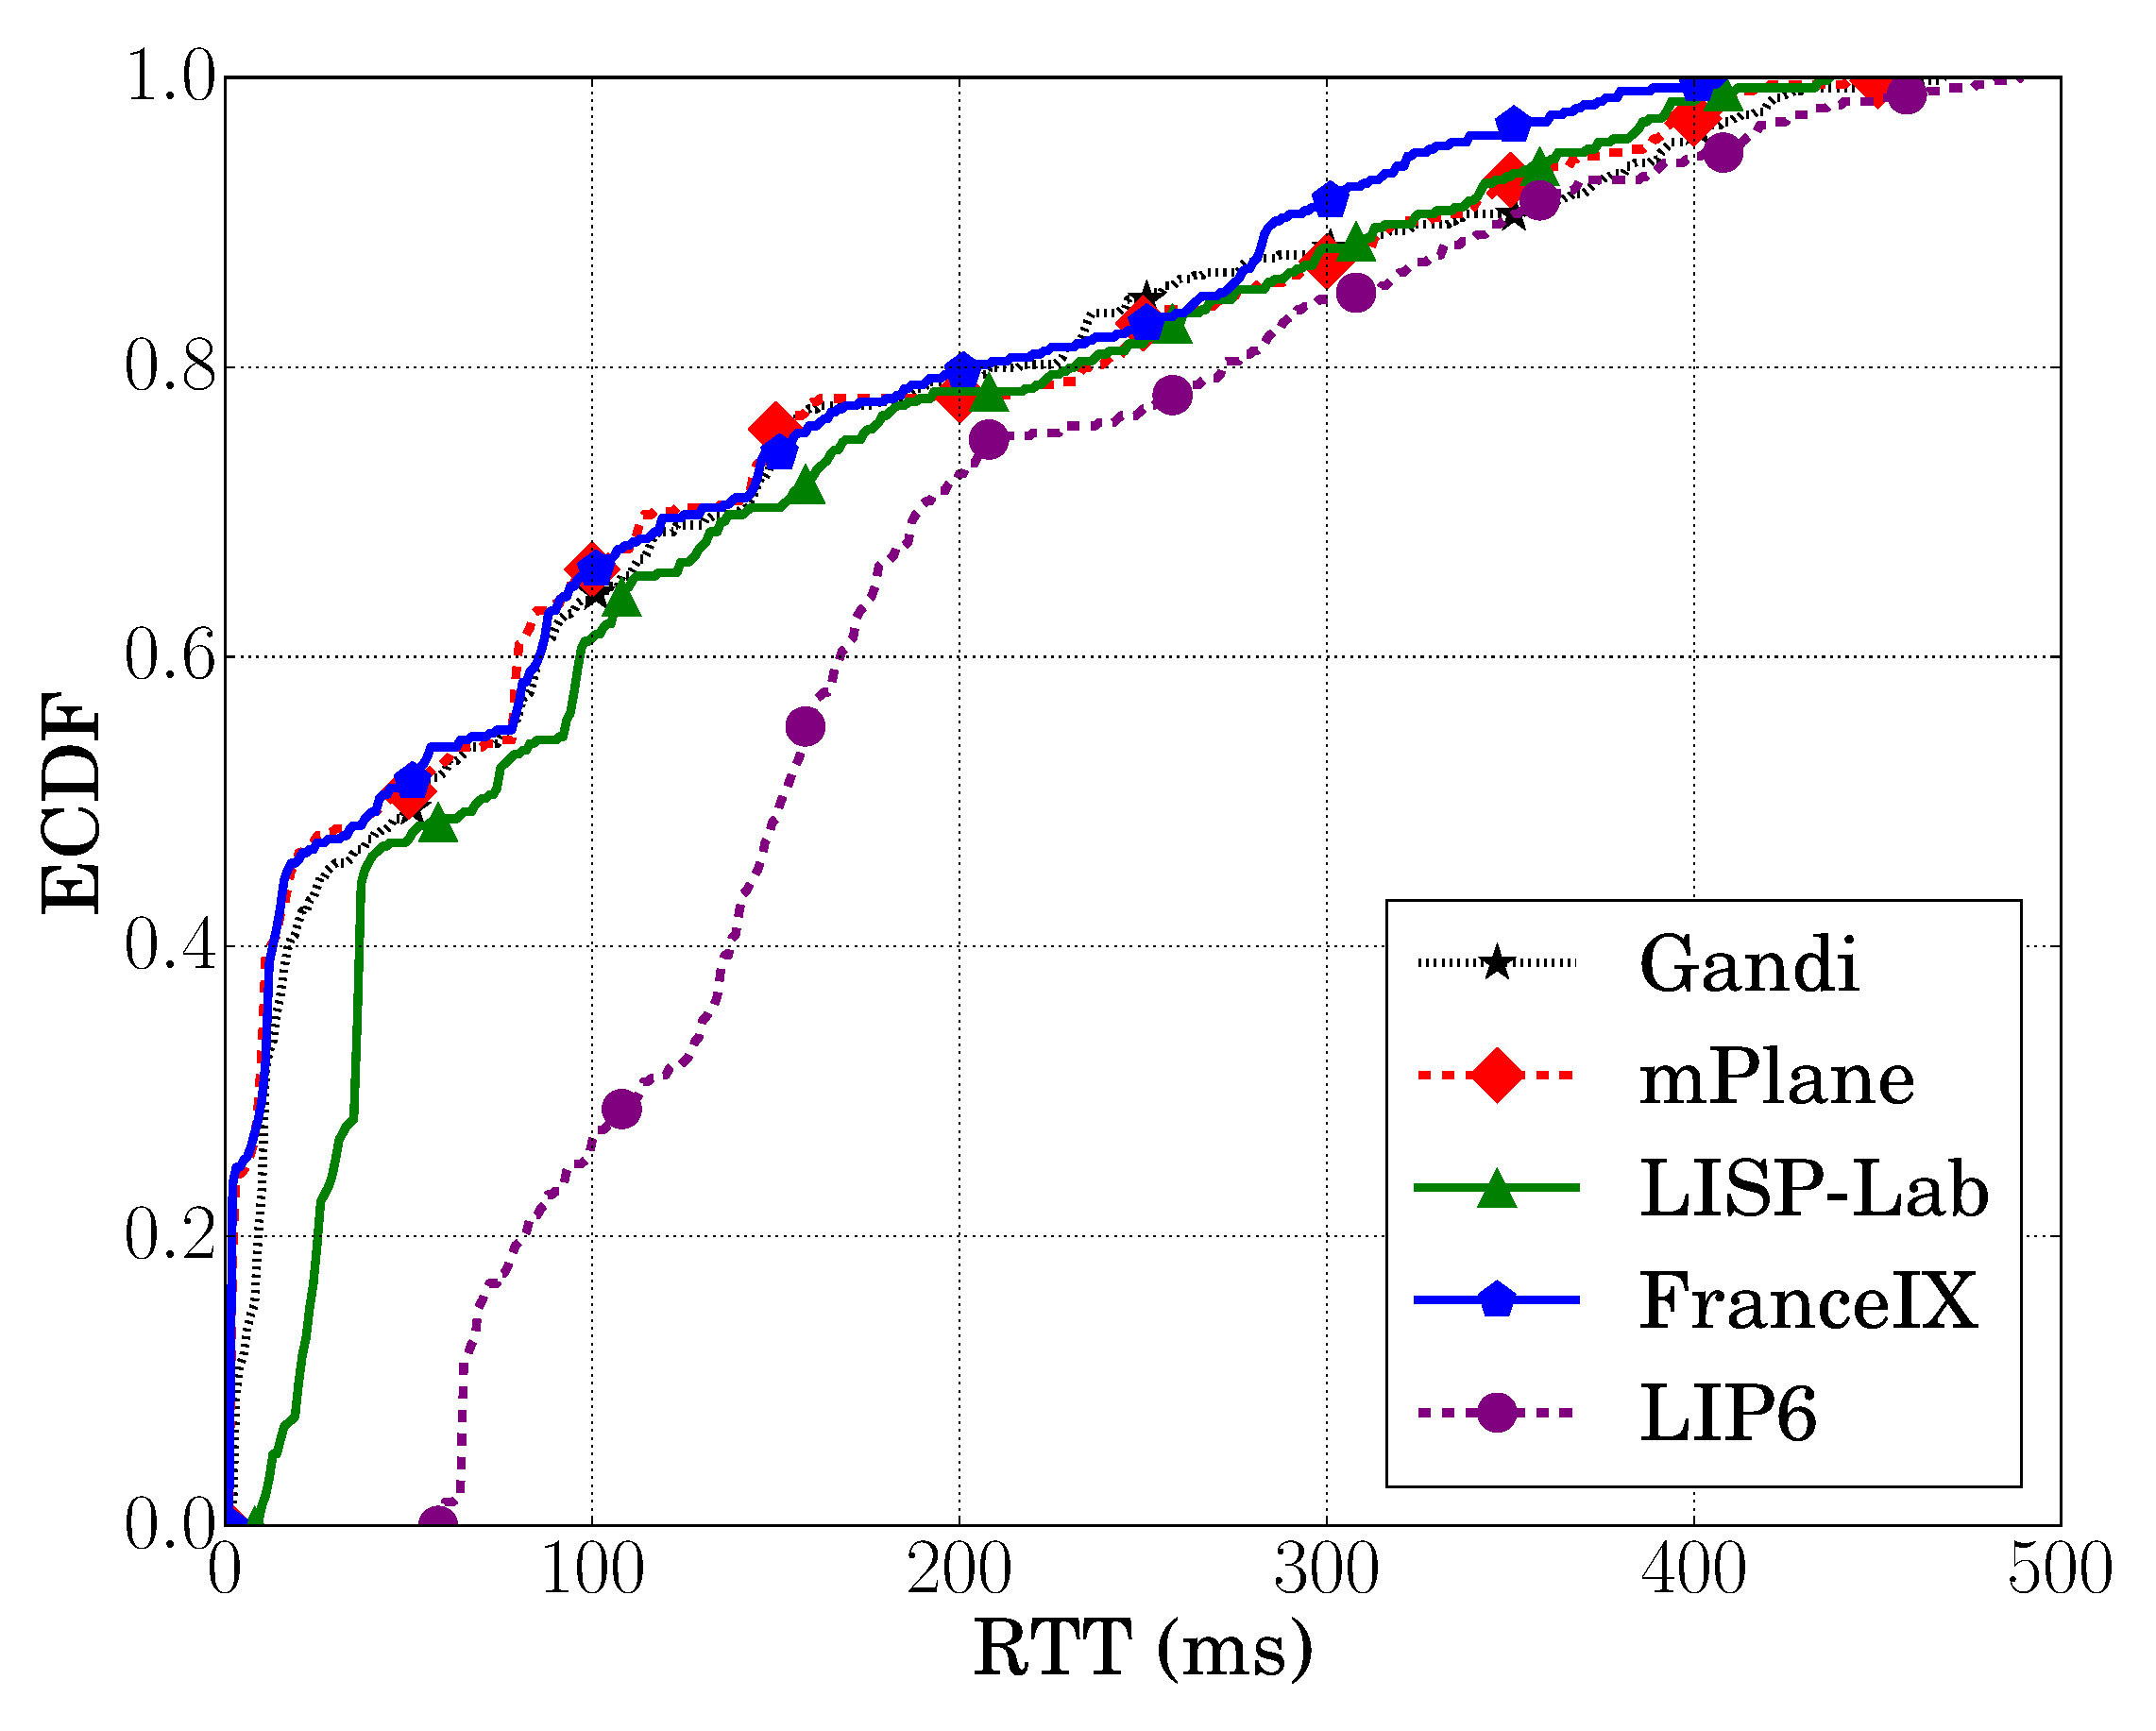
\includegraphics[width=0.6\textwidth]{Pics/v4/CDF_avg(RTT)_median_4_20.eps}
	\caption{CDF of median RTT between different probes (IPv4) from Dataset 2016}
	\label{CDF_of_median_RTT_between_different_probes_v4_2016}
\end{figure}
%-< END FIGURE >--------------------------------------------------------------------

Fig.~\ref{CDF_of_median_RTT_between_different_probes_v4_2016} shows the CDF of the average RTT toward the selected IPv4 destinations for Dataset 2016. % Because of the experimental targets are worldwide, the range of observed RTTs varies from few milliseconds (ms) to nearly 500ms. 
As an anchor, the FranceIX probe outperforms other probes in most cases, hence, showing the smallest RTT. With RTT range $[0, 200]$ ms, the latency from two LISP probes, LISP-Lab and LIP6, are respectively 25 ms and 60 ms slower than three other non-LISP probes. Such a RTT performance degradation is caused by the path length stretch introduced by the the proxy technology (as mentioned in Sec.~\ref{sec:background_lisp}), since every packet sent between LISP probe and the legacy Internet has to pass through a PxTR. Although both LISP probes introduce the stretch, LIP6 probe is even 50ms slower than the LISP-Lab probe. Given that both LISP-Lab and LIP6 probes pass through the same PETR located in Lyon, the performance degradation of LIP6 probe is due to the PITR selection for traffic from legacy Internet to LISP network. The PITRs used by LIP6 probe belongs to the LISP Beta Network and there are in total 6 available PITRs. The PITRs announce the LISP Beta prefixes to their AS peers using BGP. So different destinations select different PITRs depending on where the destinations are and lead to the reply goes through the different paths. For example, an Asian destination normally uses the PITR in Japan instead of selecting one in Europe. As listed in Tab.~\ref{PxTR_loc_2016}, LISP Beta Network has not deployed PITR in France, while the PITR of LISP-Lab is in the same country to its probe. Thus, the return path that we measured for the LIP6 probe is longer than for the LISP-Lab probe. As a result, the closer the destination is located to the probes, the bigger the difference of RTT between the two LISP probes.

Within RTT range $[200, 500]$ ms, all probes except LIP6 show basically the same RTT. It indicates that LISP-Lab has a better performance in scenario of long distance network connection. The reason is that stretch delay from LISP-Lab probe to PxTR (in Lyon) can be ignored. Fig.~\ref{CDF_of_median_RTT_between_different_probes_v4_2016} confirms this situation, within RTT range $[200, 500]$ ms, the difference between two probes becomes significantly smaller than that in range $[0, 200]$ ms.

The aforementioned results and analysis coincide with the Fig.~\ref{CDF_RTT_avg_v4_2015} from the dataset of 2015, which just covers comparison related to LISP-Lab probe. This indicates that the LISP PxTR performance is stable: the measurement results do not change with the different destinations at the different time. 

%-< FIGURE >--------------------------------------------------------------------
\begin{figure}[!t]
	\centering
	\includegraphics[width=0.6\textwidth]{Pics/v4/Smallest_median_avg(RTT)_proporation.eps}
	\caption{Smallest median RTT grouped by continent (IPv4) from Dataset 2016.}
	\label{Smallest_median_avg(RTT)_proporation_v4_2016}
\end{figure}
%-< END FIGURE >--------------------------------------------------------------------

Even with stretch brought by the PxTR, LISP probes still outperform non-LISP probes in some cases according to the measurement results. To identify these cases, worldwide destinations are classified by continent.
Fig.~\ref{Smallest_median_avg(RTT)_proporation_v4_2016} depicts the percentage of times that one probe has the smallest RTT compared to the other probes grouped by continents where the selected targets are located.
The experimental destinations are located in 4 continents, i.e., Europe, North America, South America, and Asia. The \emph{ping} measurement is repeated 720 times as the experiment lasts 15 days and its interval is 30 minutes. The RTTs of the FranceIX anchor and mPlane probe are the smallest most of the time, especially for the European and South American destinations. Only for the Asian destinations the RTT of LISP-Lab probe experiences sometimes the smallest latency for $8.82\%$ of the targets, while the LIP6 probe experiences the smallest latency in $0.98\%$ of the cases. Among the North American destinations, there is just one destination for which the RTT of the LISP-Lab probe is the smallest, while there is no destination for which LIP6 experiences the smallest latency. Fig.~\ref{CDF_of_median_RTT_between_different_probes_v4_2016} shows that for RTT above 200 ms LISP-Lab performs like the other probes, so that we can question whether it actually has the best performance in some cases, and for which destinations. Fig.~\ref{Smallest_median_avg(RTT)_proporation_v4_2016} shows the geographic location of destinations for which LISP-Lab actually is the best performing probe. In particular, the LISP-Lab probe has no additional delay compared to other non-LISP probes for the intercontinental transmission to the Asian destinations. It means that the negative effect of LISP stretch delay is evident for communications with European and American destinations, but can be neglected for Asian intercontinental destinations. This phenomenon is similar to the result shown in~\cite{li2016performance}, which shows only in $5.6\%$ of the cases that the LISP-Lab probe experiences the smallest latency and all these destinations are in Asia. It proves again that the negative effect of LISP PxTR can be ignored for the intercontinental transmission to the Asian destinations (when considering the European vantage point).

 %-< TABLE >-----------------------------------------------------------------
 %%%%%%%%%%%%%%% Table %%%%%%%%%%%%%%% 
 \begin{table}[!tb]
 	\centering
 	\caption{Correlation coefficient to FranceIX (IPv4) from Dataset 2016}
 	\label{correlation_v4_2016}{
 	\resizebox{0.65\textwidth}{!}{%
 		\begin{tabular}{@{}c|c|c|c|c|c@{}}
 			\hline\hline
 			 & Gandi  & mPlane  & LISP-Lab  & LIP6 &  FranceIX \\ \hline
 			Coefficient &  0.9647 & 0.9707 & 0.9766 & 0.8547 & 1.0     	\\  \hline\hline                 
 		\end{tabular}
 	}}
 \end{table}
 %-< END TABLE >-----------------------------------------------------------------

% As FranceIX is an enhanced probe with more measurement capacities presenting more stable performance, 
Also for the Dataset 2016, we try to evaluate the correlation in term of RTT between FranceIX and other probes. % The purpose is to see if RTT measurements are correlated or totally independent. The method is to compute the correlation coefficient for every RTT series of different probes to all destinations with the ones of FranceIX. The results are shown in Tab.~\ref{correlation_v4_2016}. The absolute value of coefficient is 1 in the case of a perfect direct linear relationship, whereas 0 in the case of no correlation at all, i.e., independent. 
The correlation coefficient of LISP-Lab is 0.9766 (> 0.8), showing a very high correlation level with FranceIX, and even higher than the correlation coefficient of all the other probes. The correlation coefficient of LIP6 is 0.8547, shows a high correlation with FranceIX as well. Both LISP probes having a high correlation with FranceIX means that while certainly introducing some overheads, LISP has quite stable performance that does not deviate from normal network operation. Such result has two sides for the performance of LISP. Good because LISP shows stability. Bad because it means that LISP experiences the same performance and failures like the normal Internet.

%-< FIGURE >--------------------------------------------------------------------
\begin{figure}[!t]
	\begin{minipage}[c]{.49\linewidth}
		\begin{center}
			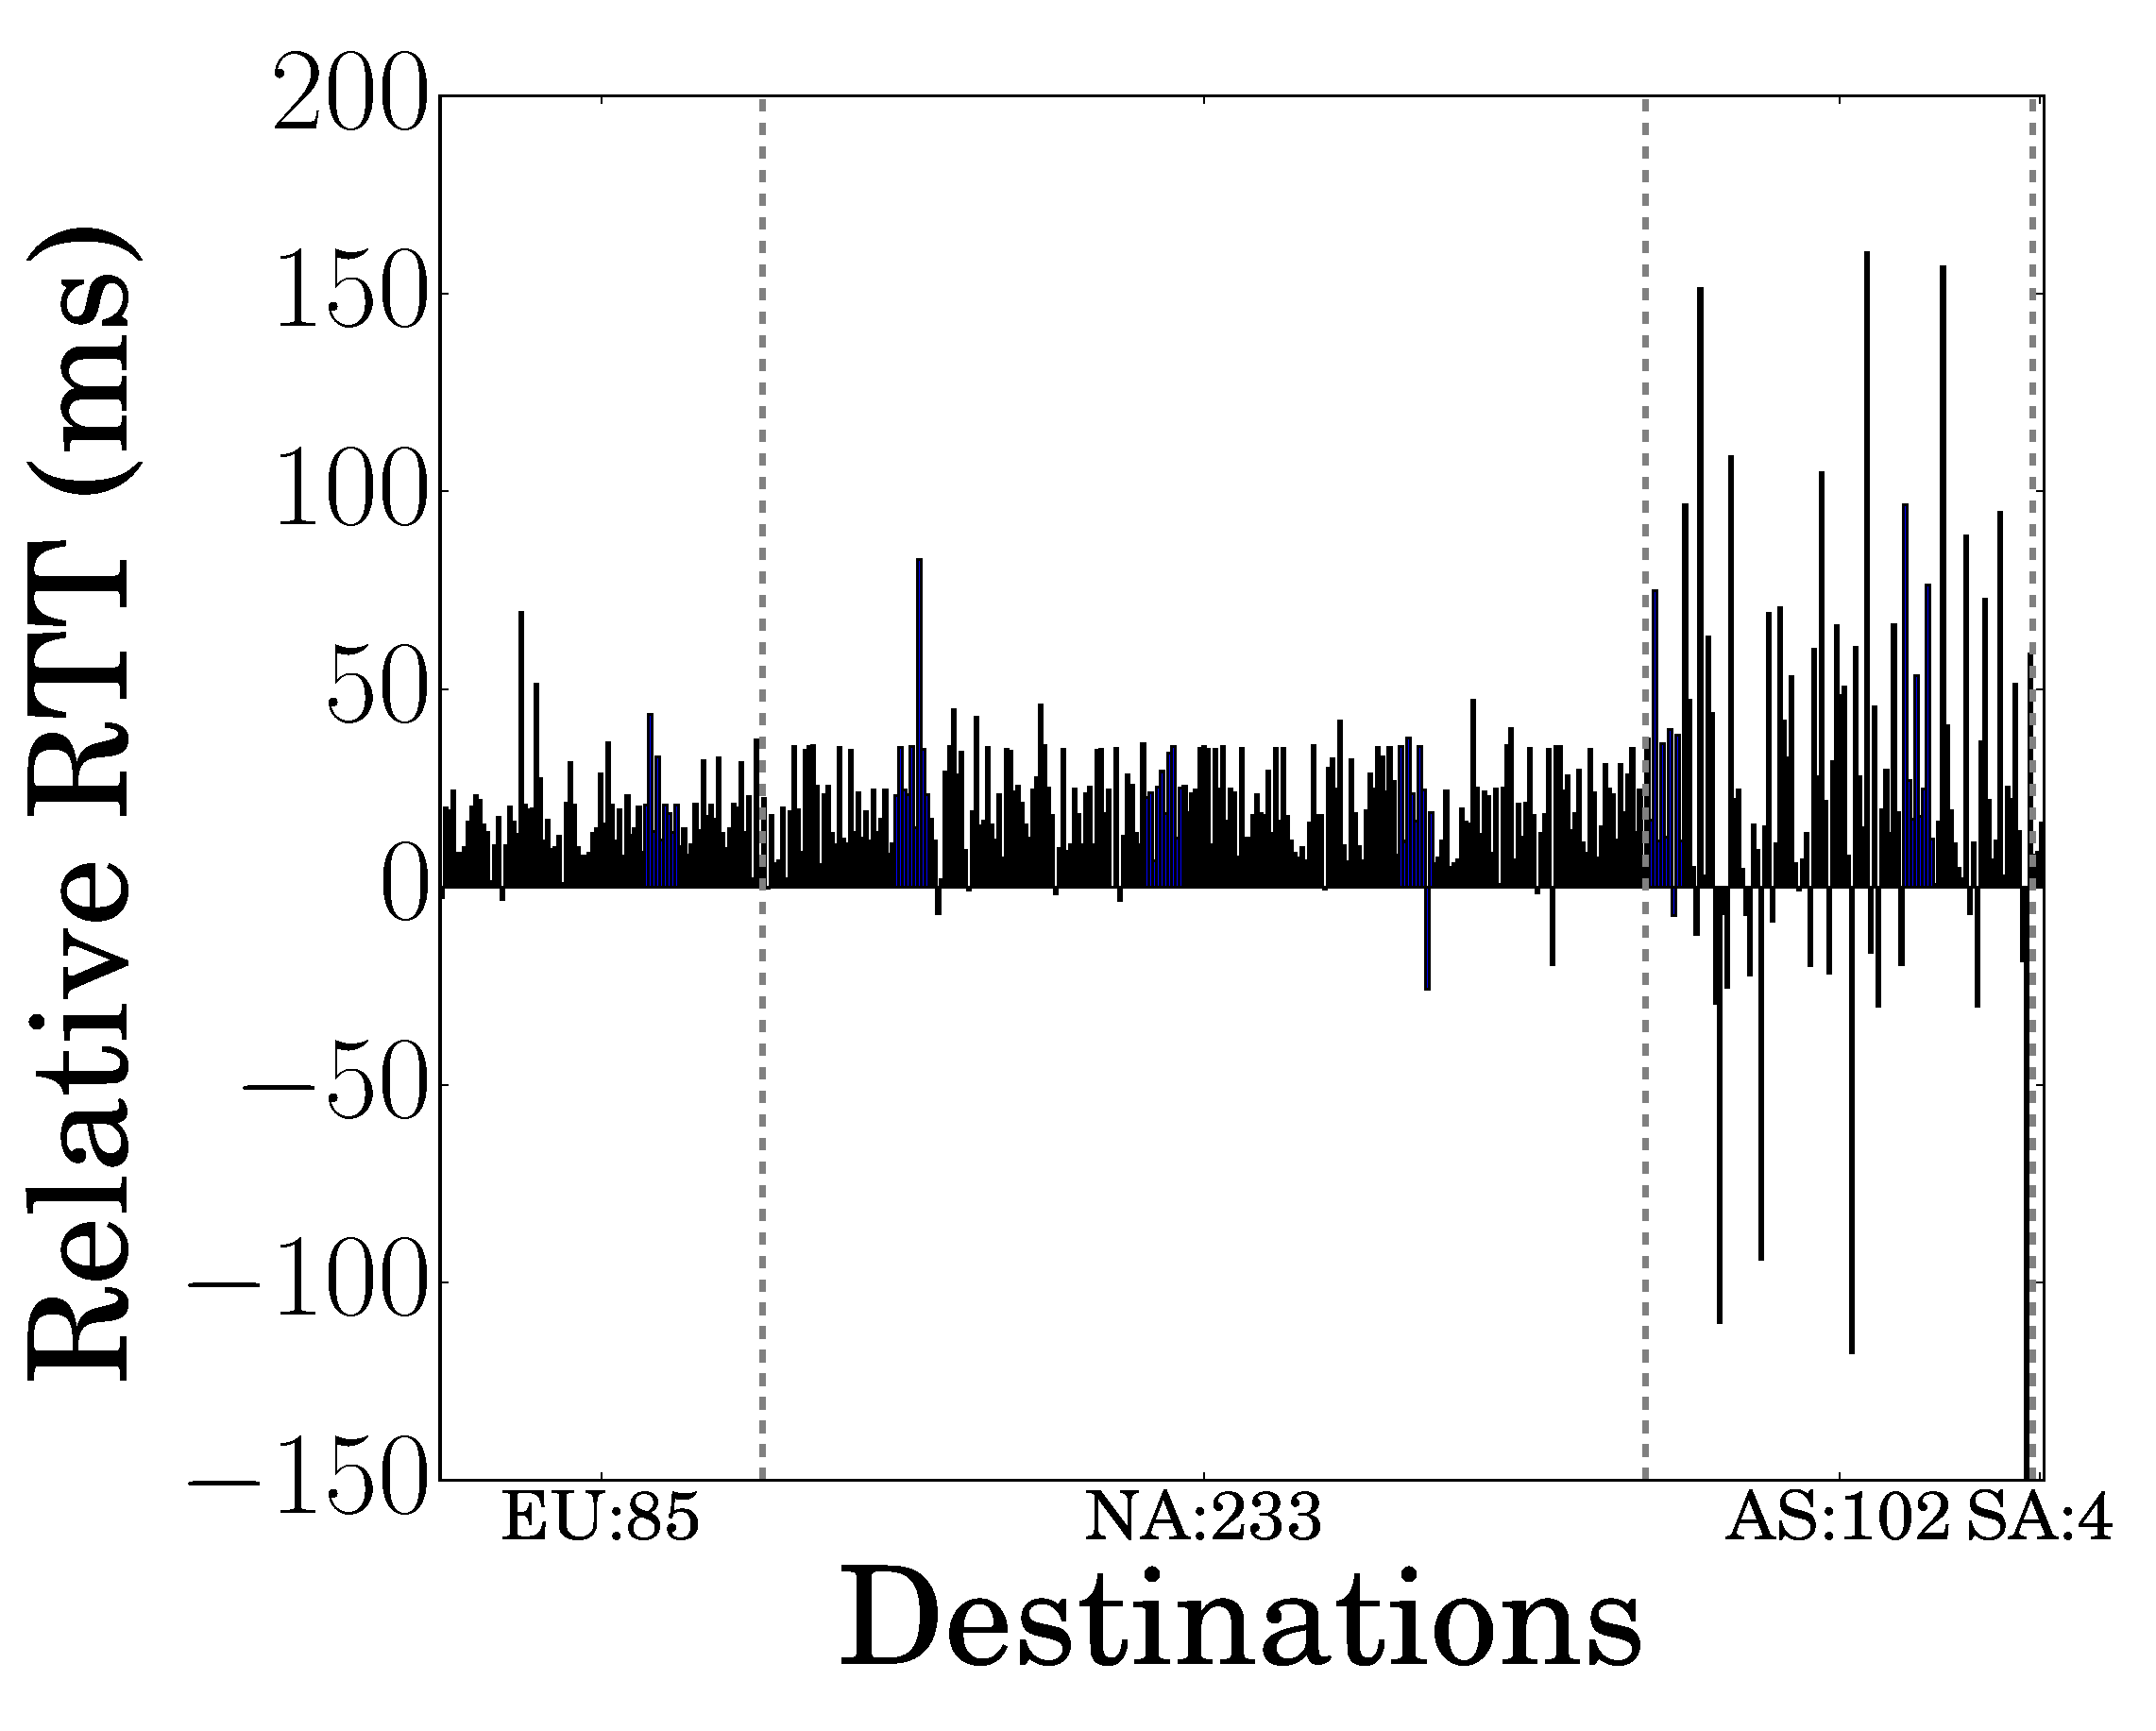
\includegraphics[width=\textwidth]{Pics/v4/Relative_median_avg(RTT)_LISP-Lab-FranceIX_changed_60.eps}
		\end{center}
	\end{minipage}
	\begin{minipage}[c]{.49\linewidth}
		\begin{center}
			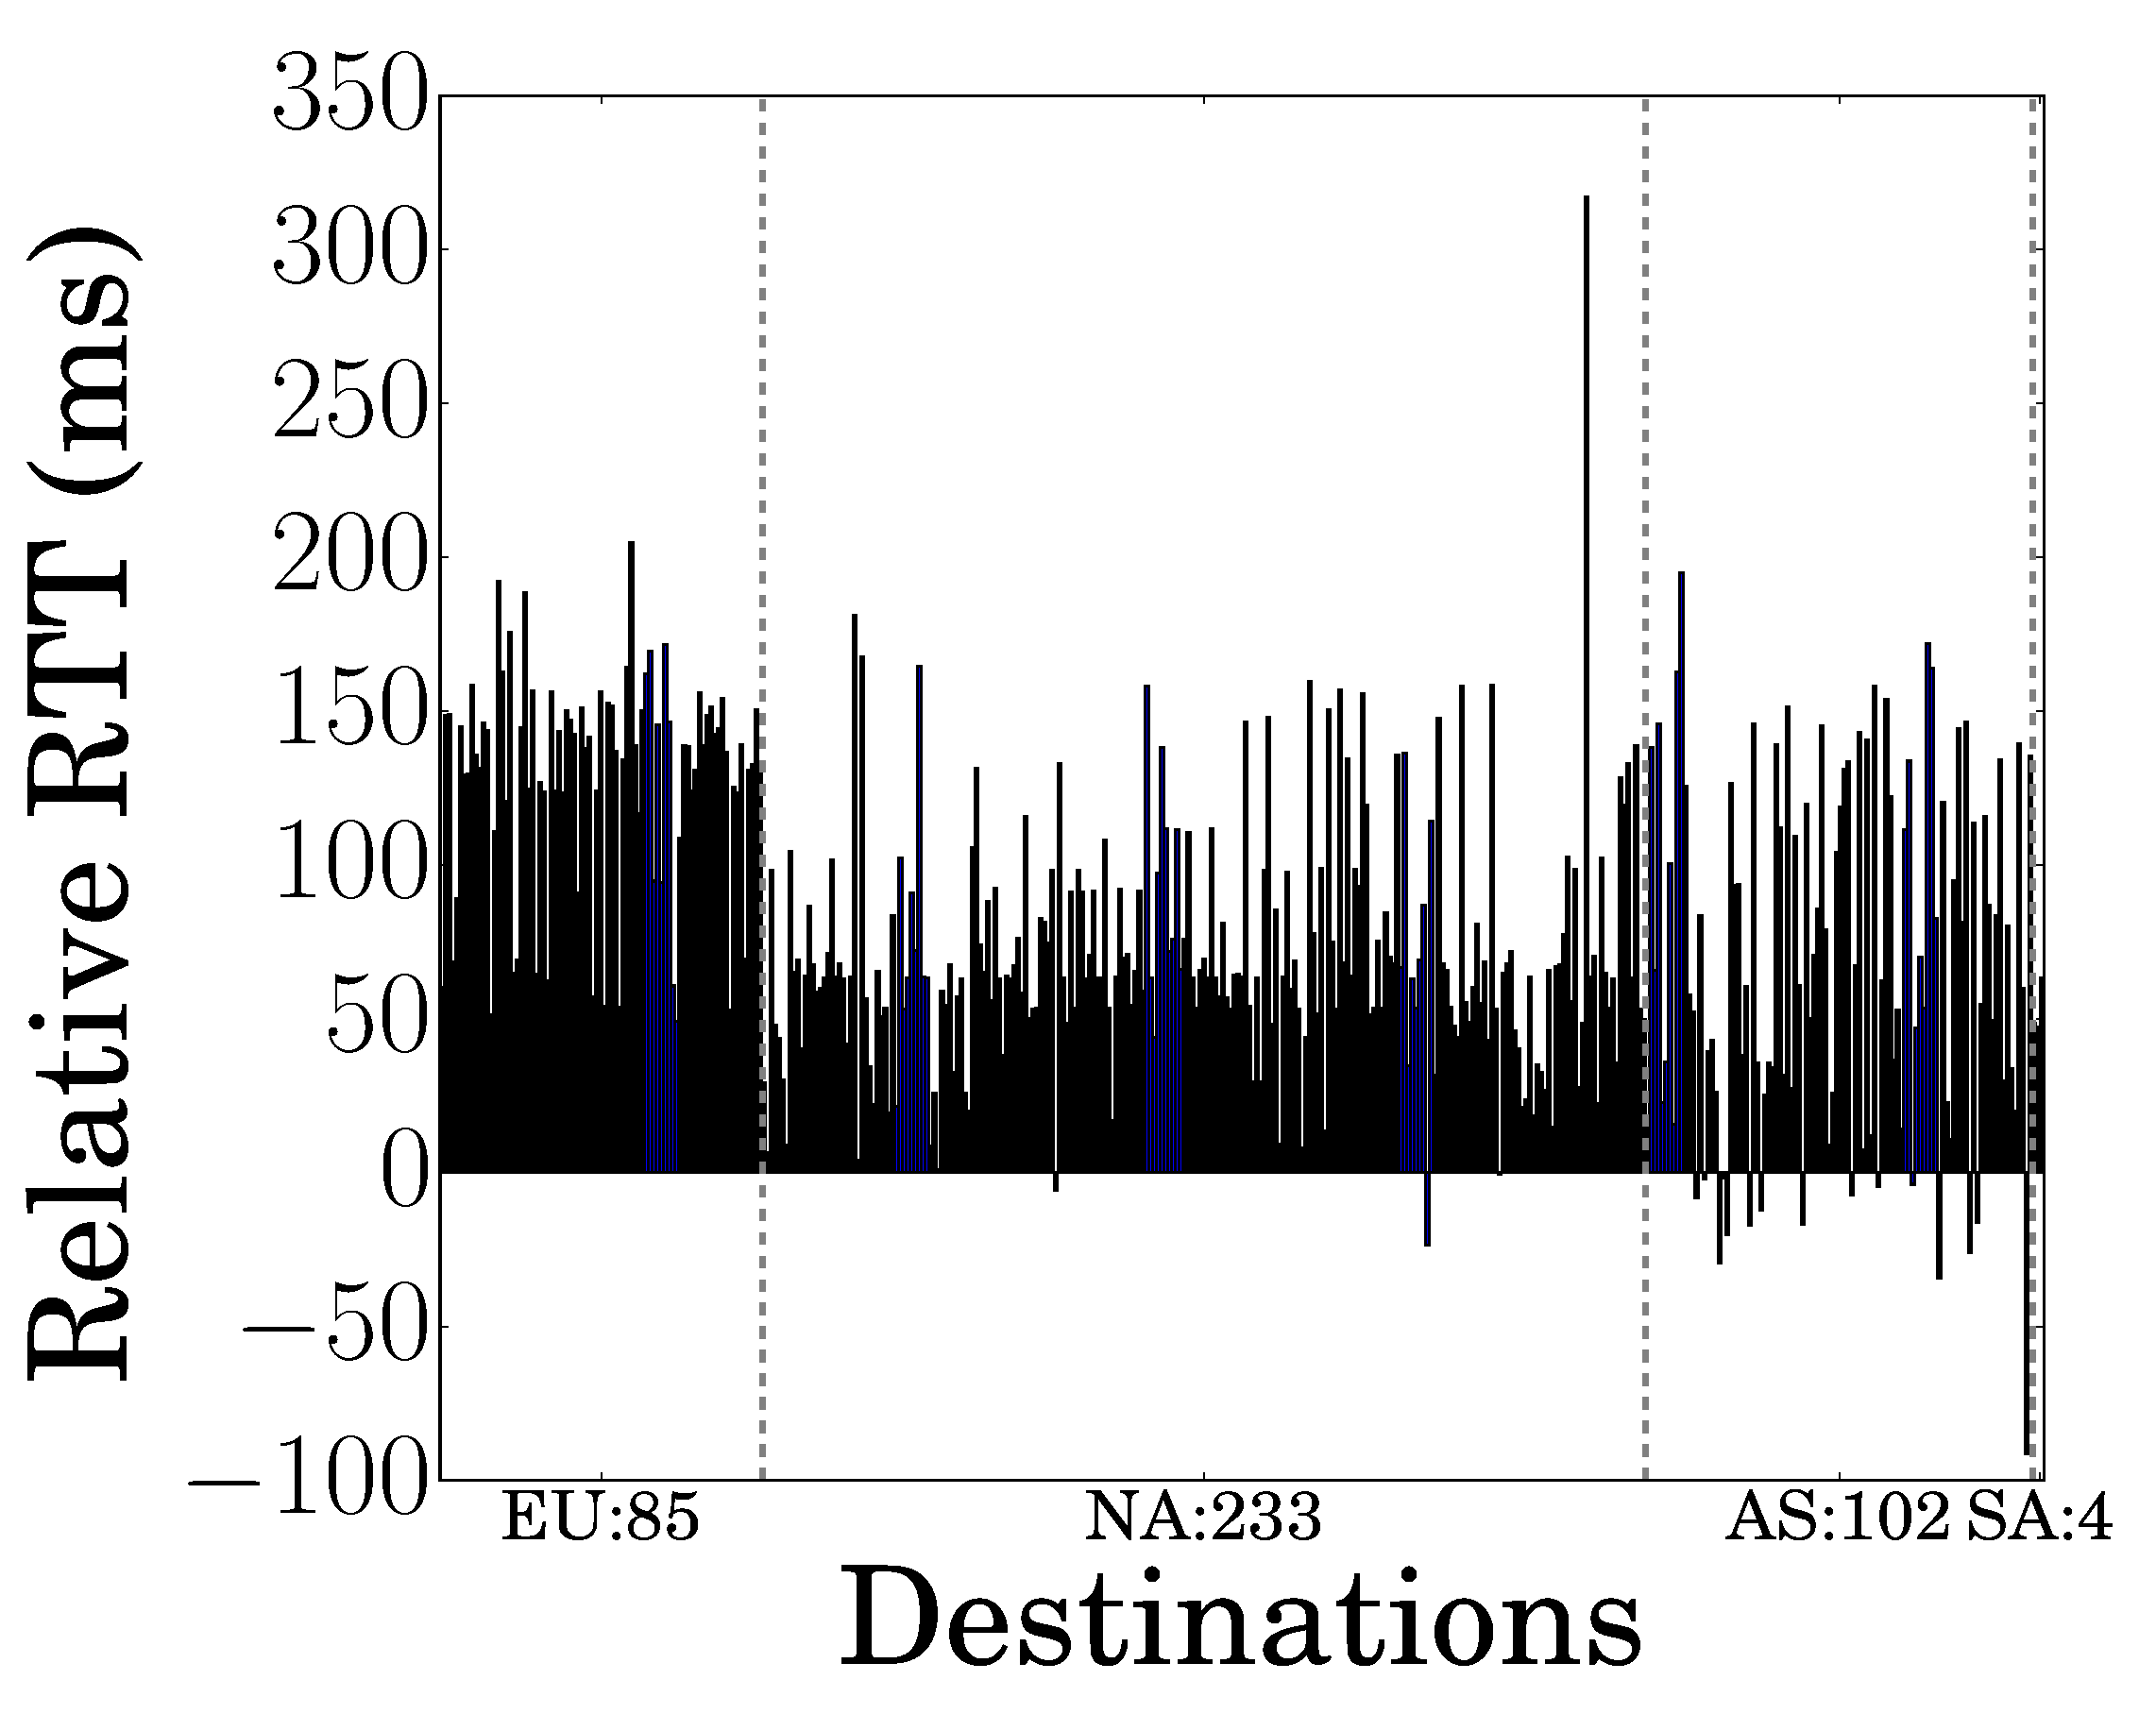
\includegraphics[width=\textwidth]{Pics/v4/Relative_median_avg(RTT)_LIP6-FranceIX_changed_60.eps}
		\end{center}
	\end{minipage}
	\vspace{-0.5mm}
	\caption{IPv4 Relative median RTT clustered by different continents for LISP-Lab (left) and LIP6 (right) from Dataset 2016}
	\label{Relative_median_avg(RTT)_v4_2016}
\end{figure}
%-< END FIGURE >--------------------------------------------------------------------
Another interesting point is to asses whether the two LISP probes have a stable performance as FranceIX according to the destinations. To this end, we leverage on the same metric of \emph{Relative RTT (rRTT)} (formula~\ref{rRTT_ll_2015}), defined in Sec.~\ref{sec:pxtr_ping_v4_2015} for each destination as: 
\begin{equation} 
    \label{rRTT_ll_2016}
    rRTT_{LL}(d)=RTT_{LL}(d) - RTT_{F}(d)
\end{equation}
\begin{equation}
    \label{rRTT_l6_2016}
    rRTT_{L6}(d) = RTT_{L6}(d) - RTT_{F}(d)
\end{equation}
where $d$ is the destination, subscriptions $LL$, $L6$ and $F$ respectively refers to LISP-Lab, LIP6 and FranceIX. The results clustered by continents are shown in Fig.~\ref{Relative_median_avg(RTT)_v4_2016}, where the relative RTT for LISP-Lab probe is on the left and the relative RTT for LIP6 probe is on the right. The positive relative RTT indicates FranceIX faster, while the negative values indicating that LISP-Lab or LIP6 are faster. In the left side of Fig.~\ref{Relative_median_avg(RTT)_v4_2016}, for the European and American targets, the values are between 10 ms and 20 ms in most cases (i.e., 31.37\%), showing that LISP-Lab is a little slower than FranceIX but with a stable behavior. On the contrary, for some Asian destinations, LISP-Lab is significantly either faster (in $20.6\%$ of the cases) or slower than FranceIX and the largest difference reaches 150 ms. It shows as well that for the European and American targets, LISP-Lab probe is stable compared to FranceIX, since the difference is mainly caused by the transmission delay between Paris (location of probe) and Lyon (location of PxTR). But when considering the Asian destinations, LISP-Lab does not show a very stable behavior, where the difference might be very large, since the path diversity for long-distance intercontinental transmission is higher, with every path having very different performance. The right figure of Fig.~\ref{Relative_median_avg(RTT)_v4_2016} shows that for LIP6 probe the difference is almost always positive. For the European destinations, the average relative RTT is around 130 ms and much higher than those in the other 3 continents. All European targets show that the LIP6 probe is significantly slower than the FranceIX anchor. For the American destinations, most relative RTT decreases to around 50 ms but some of them are around 150 ms. For the Asian targets, the relative RTT presents big differences. Some still stay at around 150 ms, some drop to below 50 ms, and there are 5 destinations even show negative relative RTTs. The reasons causing the relative RTTs for LIP6 probe varying a lot are similar to that for LISP-Lab but not totally the same. The same point is that the longest transmission of traffic in our experiment are the destinations located in Asia. Since the stretch can be ignored in the case of intercontinental transmission, both of two LISP probes are not always slower than FranceIX to Asian targets. The different performance between LISP-Lab probe and LIP6 probe is caused by the location of each PxTR. Although the PxTR of LISP-Lab is not close to its probe, but at least they are in a same country. While the LIP6 probe uses the same PETR to LISP-Lab probe but its PITR is not in France, and is even quite far away. As a result, for the shorter transmission, i.e., to the European destinations, the LIP6 probe introduces extremely higher RTTs than the non-LISP probes and even higher than LISP-Lab probe. Thus, the location of PxTR is very important. The PxTR near to either the sources or the destinations can obviously decrease the stretch. At least the probe having a PxTR in the same country shows a better performance compared to the PxTR just in the same continent.

%-< TABLE >-----------------------------------------------------------------
%%%%%%%%%%%%%%% Table %%%%%%%%%%%%%%% 
\begin{table}[!tb]
	\centering
	\caption{Reliability of each probe (IPv4) from Dataset 2016}
	\label{reliability_v4_2016}{
	\resizebox{0.65\textwidth}{!}{%
		\begin{tabular}{@{}c|c|c|c|c|c@{}}
			\hline\hline
			& Gandi  & mPlane  & LISP-Lab  & LIP6 &  FranceIX \\ \hline
			Reliability (\%) &  99.66 & 99.65 & 99.43 & 77.78 & 99.62     	\\  \hline\hline                 
		\end{tabular}
	}}
\end{table}
%-< END TABLE >-----------------------------------------------------------------


We also want to evaluate the \emph{Reliability} when having the response to each ping measurement. We measure reliability, in our experiment, by simply calculating the percentage of replies over the total number of requests. If every ping measurement is successful, i.e., there is a response having the RTT value for a probe at every experiment round, its reliability is $100\%$. As shown in Tab.~\ref{reliability_v4_2016}, except for the LIP6 probe with $77.78\%$, all the other probes are more than $99\%$. The lower reliability of LIP6 probe indicates that sometimes its ping measurement is not successful. Since it is much lower than the others, to make sure that the LIP6 probe works well and there is no congestion or misconfiguration on the probe or any of its connected routers, we conduct another experiment letting the LIP6 probe use a normal public IPv4 address pinging the same 500 destinations. In this case, the LIP6 probe is non-LISP-speaking. The results show that the reliability of LIP6 probe is 98.91\%, which is very close to the other probes. Thus, we eliminate the possibility of the problem on the LIP6 probe itself. As the LIP6 probe uses the same PETR to the LISP-Lab probe, while the reliability of LISP-Lab is very high, the difference is caused by the PITRs. The LISP-Lab probe uses the PITR of LISP-Lab platform but the LIP6 probe leverages one of LISP Beta Network. On one hand, LIP6 probe has longer transmission distance causing more risk of losing the packets and thus leads to more losses. On the other hand, we can conclude that the performance of LISP-Lab PxTR is more reliable than that of LISP Beta Network.

Since the experiment in 2015 just lasts 6 hours and shows no periodicity. Thus, this experiment campaign is extended to conduct with a span of 2 weeks to assess whether the RTT measurements have periodicity. Two methods are used to check: Fast Fourier transform (FFT) and Auto-correlation. However, the analysis results also show that none of RTT series from probes to any destinations exhibits periodicity. It means that the traffic does not periodically fluctuate with a certain interval.


\section{IPv6 Ping results}
\label{sec:pxtr_ping_v6}
% \begin{itemize}[noitemsep,topsep=0pt]
%     \item CDF of median RTT between different probes
%     \item Smallest median RTT grouped by continent
%     \item Correlation coefficient to FranceIX
%     \item Relative median RTT clustered by continent for LISP-Lab and LIP6
%     \item Reliability of each probe
%     \item The periodicity check
% \end{itemize}
%-< FIGURE >--------------------------------------------------------------------
\begin{figure}[!t]
	\centering
	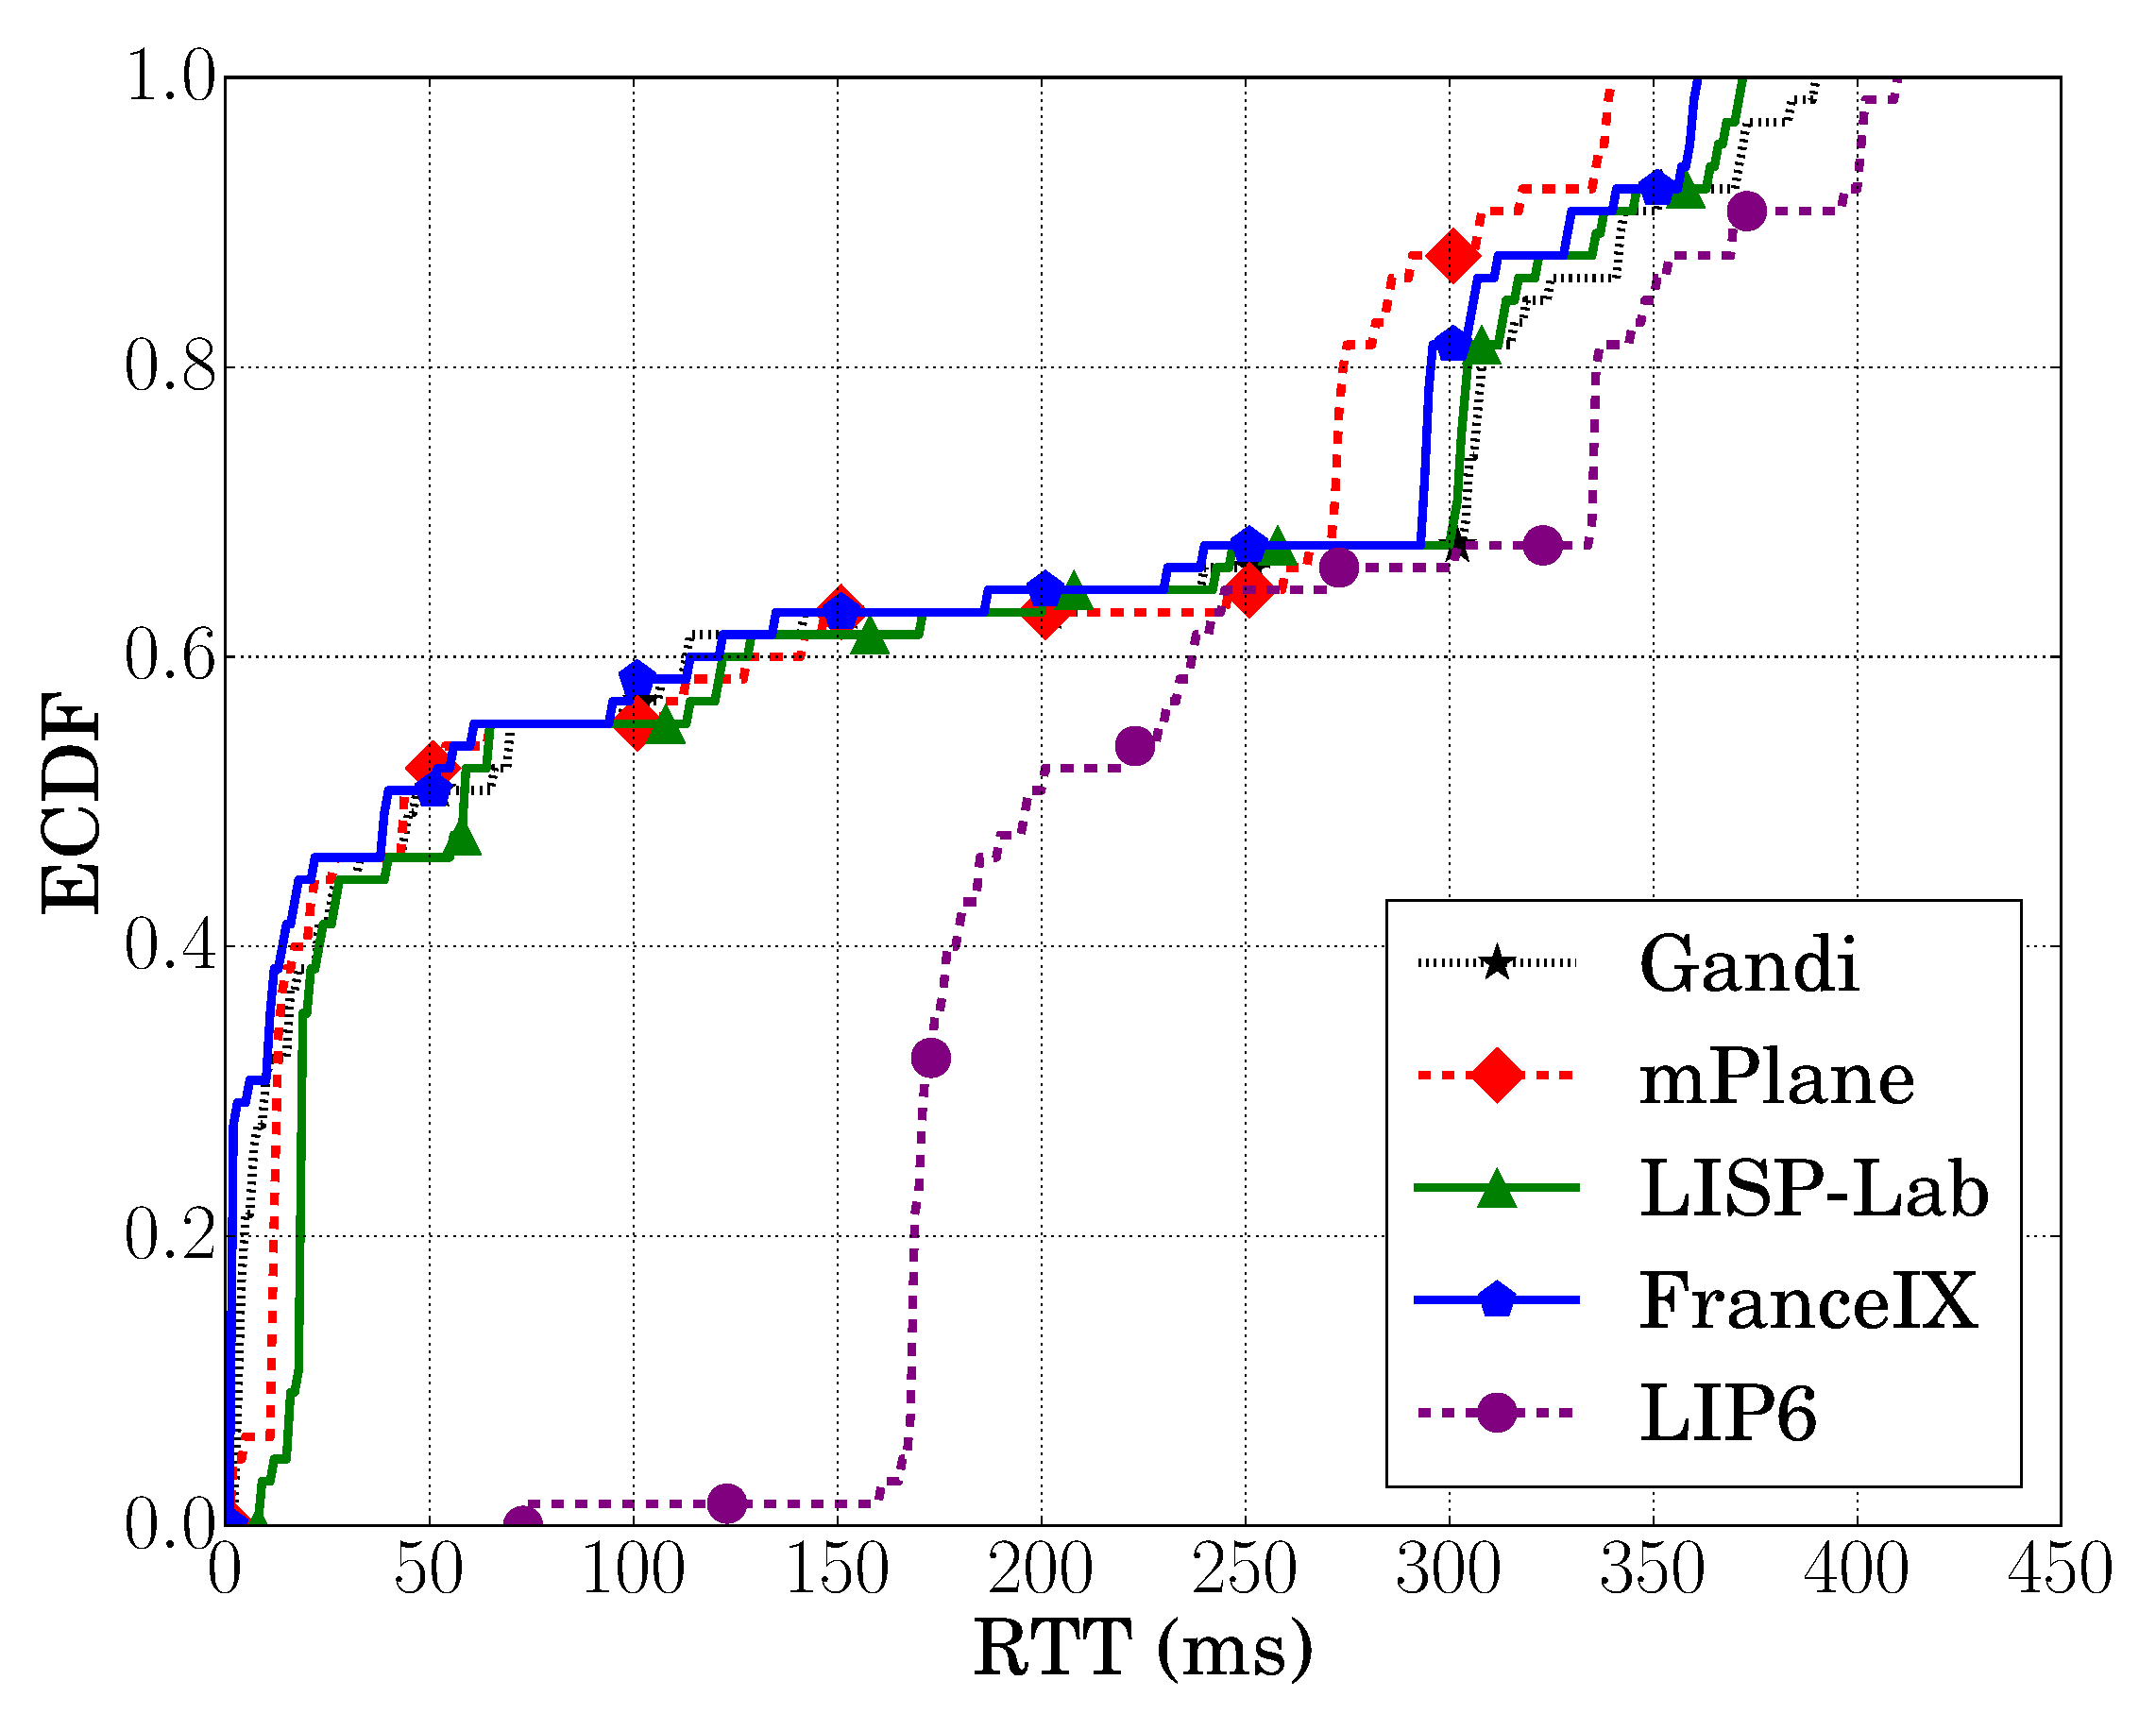
\includegraphics[width=0.6\textwidth]{Pics/v6/CDF_avg(RTT)_median_4_20.eps}
	\caption{CDF of median RTT between different probes (IPv6) from Dataset 2016}
	\label{CDF_of_median_RTT_between_different_probes_v6_2016}
\end{figure}
%-< END FIGURE >--------------------------------------------------------------------

In this section, LISP interworking performance of IPv6 is evaluated with the same metrics as those used in Sec.~\ref{sec:pxtr_ping_v4_2016}.

The CDF of average RTTs to the selected IPv6 destinations is shown on Fig.~\ref{CDF_of_median_RTT_between_different_probes_v6_2016}, which is generally similar to the Fig.~\ref{CDF_of_median_RTT_between_different_probes_v4_2016} for IPv4. The FranceIX anchor still shows the best performance with the smallest delay for almost all the destinations. The RTT of LISP-Lab probe is always higher than the other non-LISP probes with RTT range $[0, 30]$ ms and the difference is around 7 ms. The RTTs are almost the same when the values are more than 30 ms. Hence, the performance of IPv6 is similar to IPv4 that the stretch introduced by PxTR is significant when the range of RTT value is small, but can be ignored when the range of RTT value becomes large. 

However, in the experiment for IPv6 targets, the traffic produced by LISP-Lab probe are natively forwarded to the destinations instead of going to the PETR in Lyon first, thus the RTT difference compared to the other non-LISP probes becomes smaller compared to those for IPv4. But the latency still exists, caused by the returning traffic that still need to pass through a PITR. Since the latency decreases, it is easier to be ignored for IPv6. That is the reason why the stretch can be ignored when RTT values are higher than just 30 ms for IPv6 while it needs to be higher than 200 ms for IPv4. While the LIP6 probe is always the slowest compared to the other probes, the difference is even 160 ms to the non-LISP probes and 150 ms to the LISP-Lab probe. The reason having such a big difference is not only caused by the bidirectional traffic should pass through the PxTR, but also caused by the route between xTR of LIP6 probe to the PETR at Lyon, which has no tunnel indicating the used routing path longer than the case of having an MPLS tunnel. Similar to IPv4, when RTT values are higher than 250 ms, the difference decreases to 40 ms in most cases.

%-< FIGURE >--------------------------------------------------------------------
\begin{figure}[!t]
	\begin{minipage}[c]{.49\linewidth}
		\begin{center}
			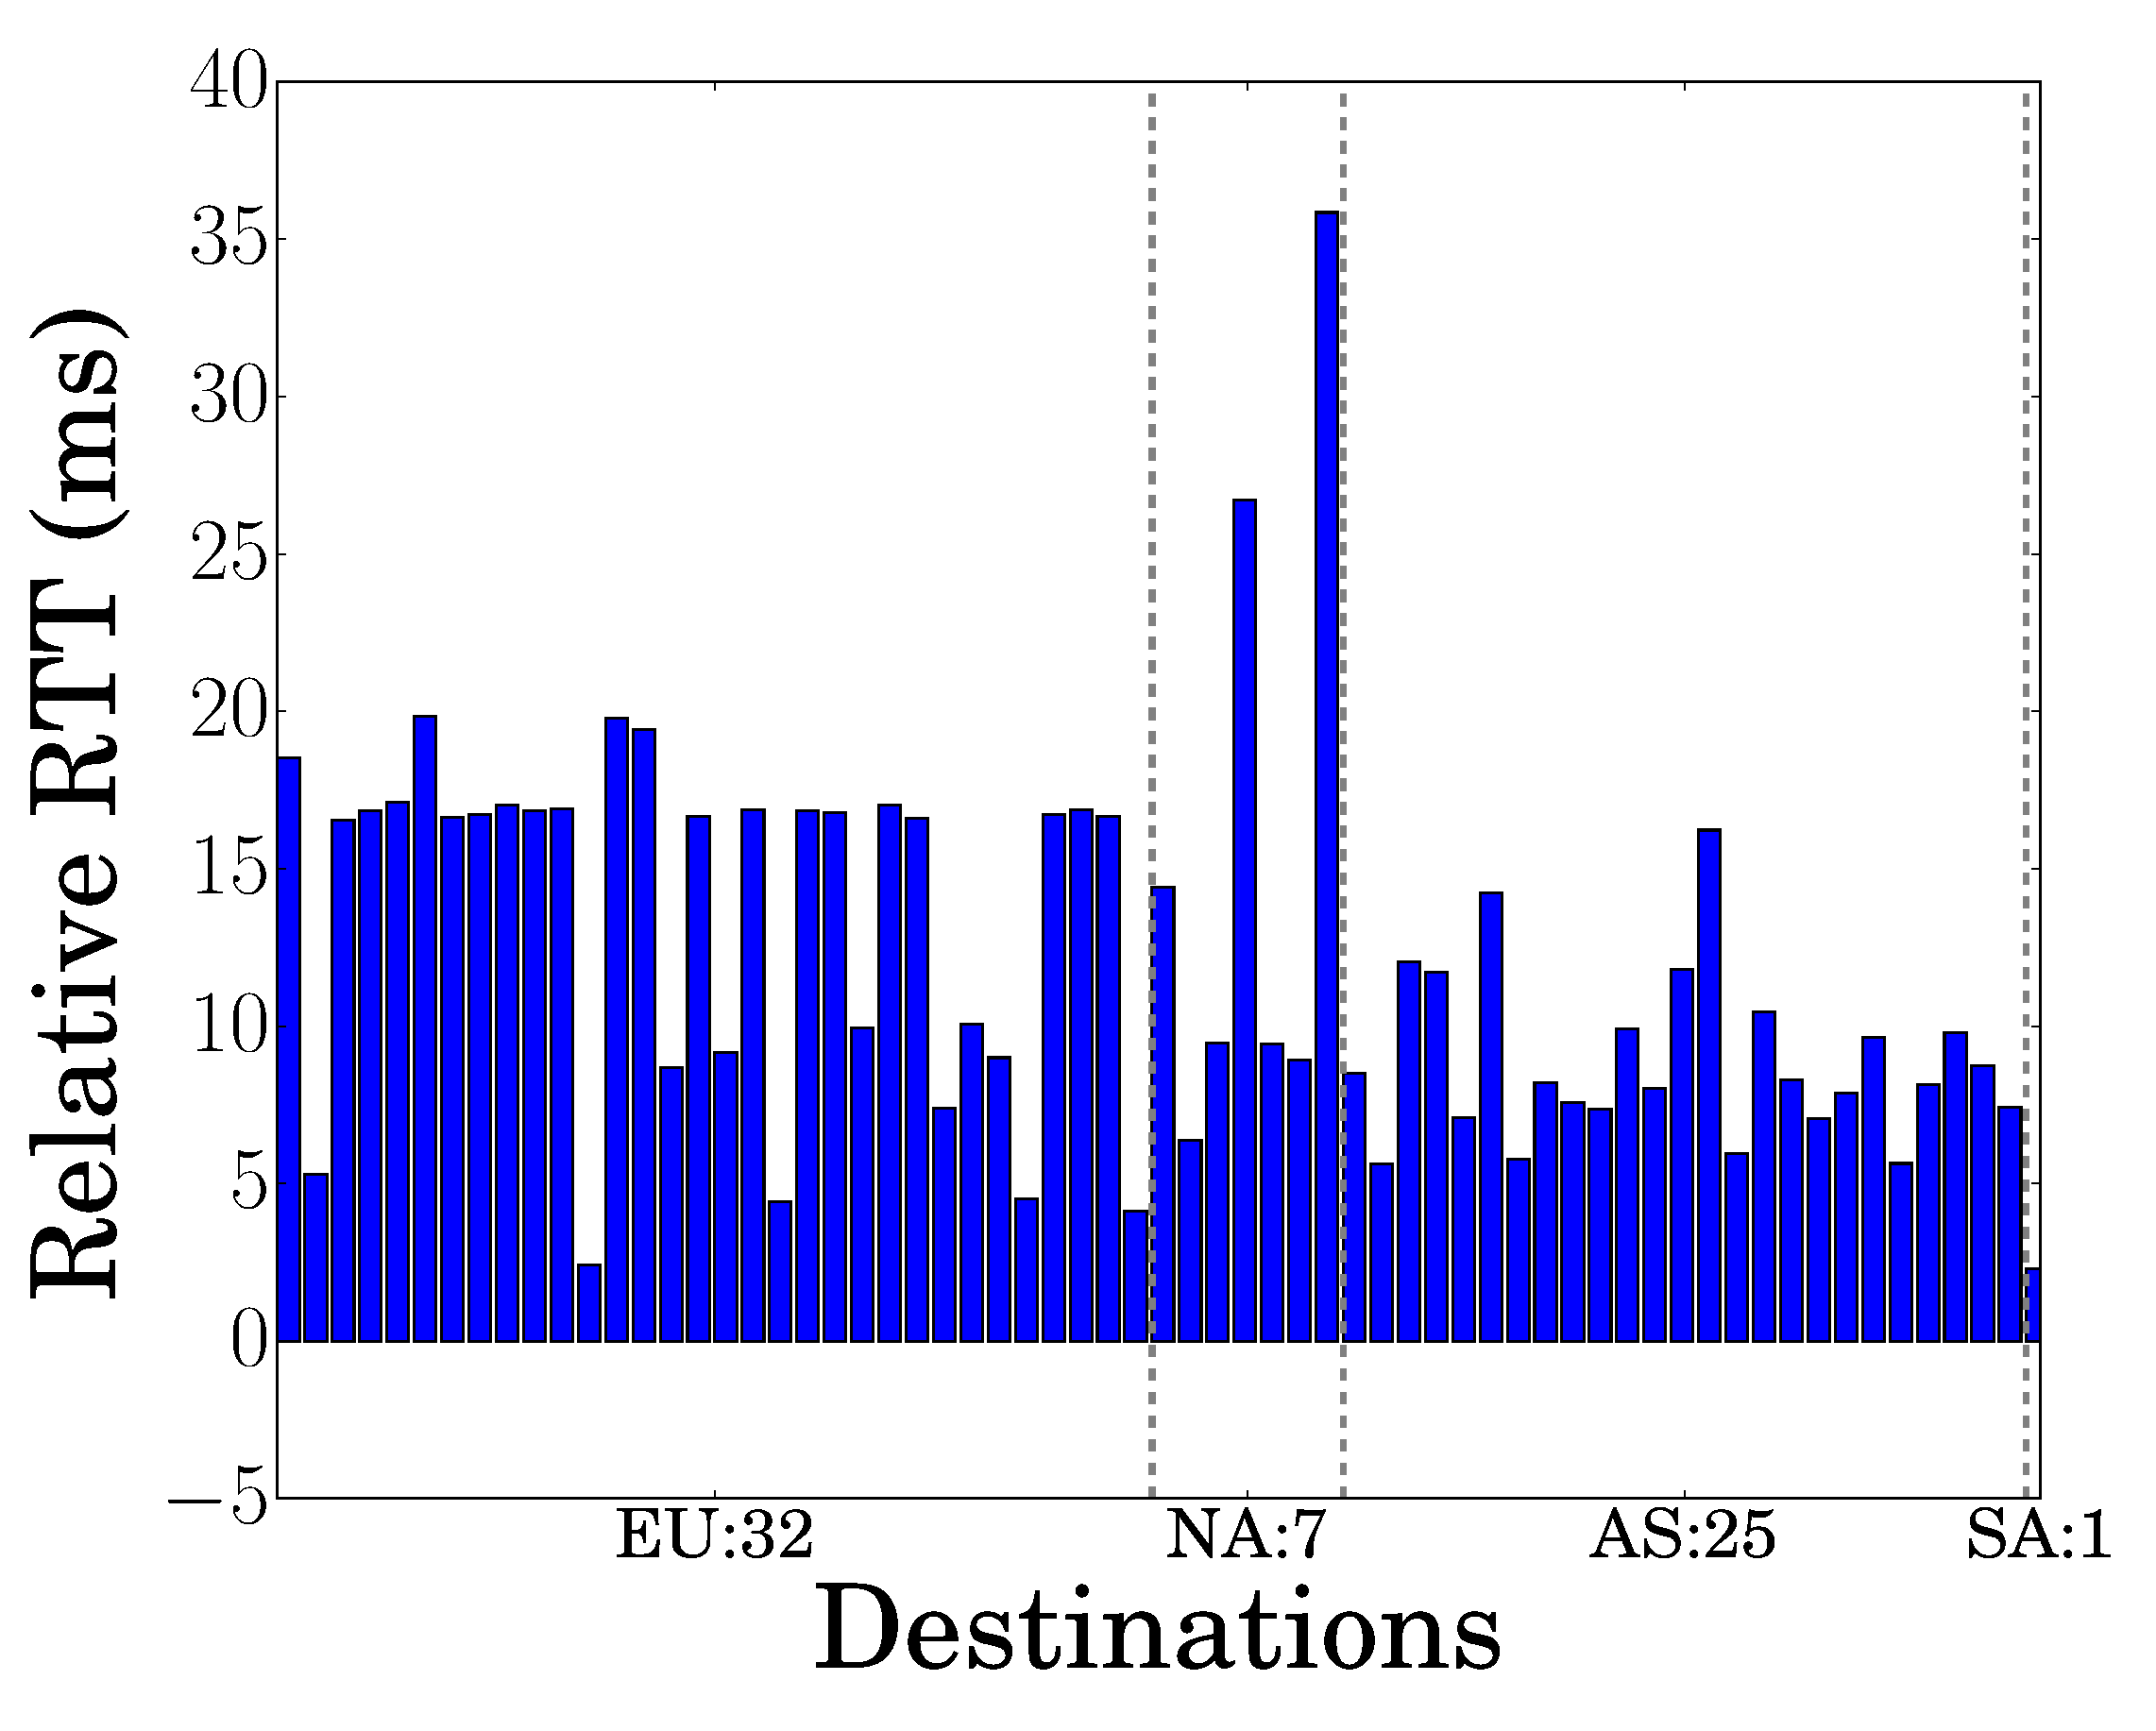
\includegraphics[width=\textwidth]{Pics/v6/Relative_median_avg(RTT)_LISP-Lab-FranceIX.eps}
		\end{center}
	\end{minipage}
	\begin{minipage}[c]{.49\linewidth}
		\begin{center}
			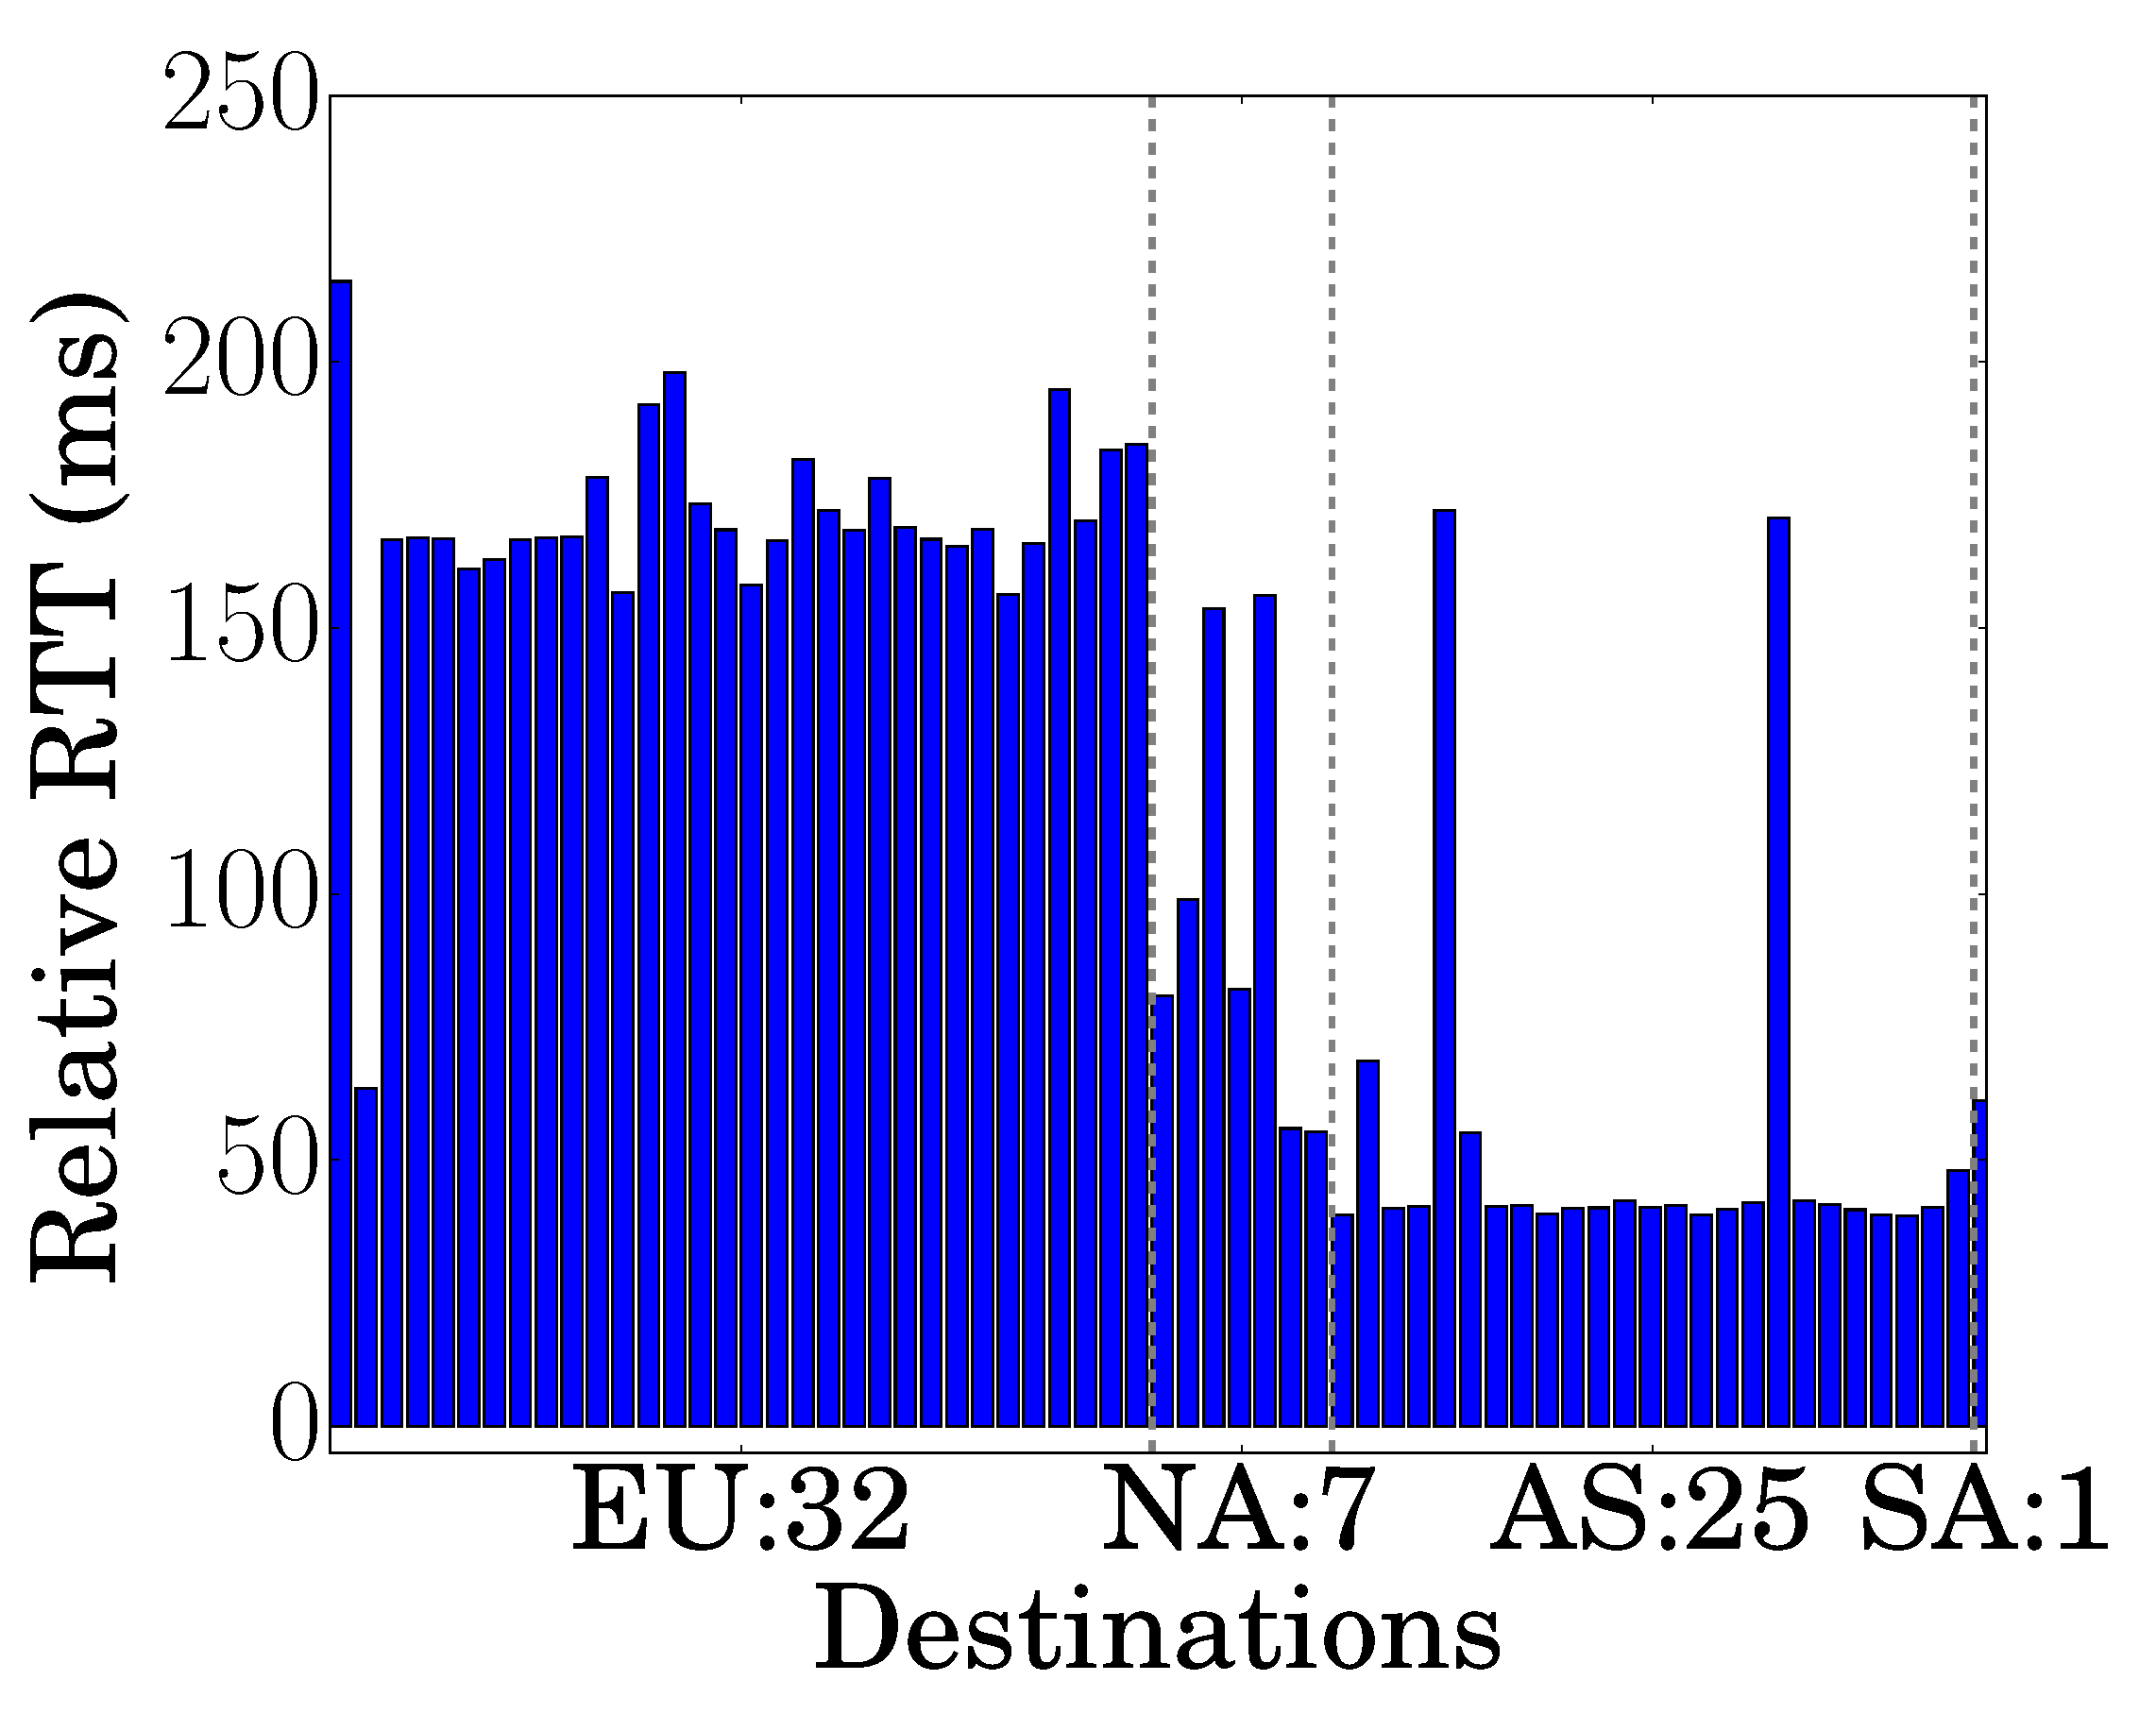
\includegraphics[width=\textwidth]{Pics/v6/Relative_median_avg(RTT)_LIP6-FranceIX_changed_60.eps}
		\end{center}
	\end{minipage}
	\vspace{-0.5mm}
	\caption{IPv6 Relative median RTT clustered by different continents for LISP-Lab (left) and LIP6 (right) from Dataset 2016}
	\label{Relative_median_avg(RTT)_v6_2016}
\end{figure}
%-< END FIGURE >--------------------------------------------------------------------
To further explore why two LISP probes are slower, especially to understand why the LIP6 probe has an extremely large latency compared to the others, we leverage on the Relative RTT between both LISP probes and the FranceIX anchor grouped in four continents as mentioned in Sec.~\ref{sec:pxtr_ping_v4_2016}. In the left figure of Fig.~\ref{Relative_median_avg(RTT)_v6_2016}, which is the relative RTT between LISP-Lab and FranceIX, all the values are positive, indicating that the LISP-Lab probe is slower than the FranceIX anchor no matter to which destination. For the European and North American targets, the relative RTTs are mostly between 5 ms and 17 ms. But the average relative RTTs decrease to 7 ms for the 25 Asian destinations. It proves the fact that for the nearby transmission, the delay introduced by PxTR is significant, while it effects less for the intercontinental transmission to the Asian destinations. What's more, the absolute relative RTT values for IPv6 are smaller than those for IPv4, because there is only returning traffic passing PITR for IPv6 so to reduce the latency. Thus, natively forwarding is faster than using PETR, but not so much. From the Fig.~\ref{Relative_median_avg(RTT)_v6_2016} we also know that there are 32 destinations located in Europe and just 7 in North America. It explains the reason why the curve of CDF for LISP-Lab sharply increases when the RTT is in the small range and mixes with the other non-LISP lines so quickly. It is because a half of destinations are not far away from the probes. Thus, a high percentage (around $50\%$) consists of small RTT values and these RTTs of LISP-Lab have a consistent delay compared to the other non-LISP probes. The mix part is mainly produced by the Asian destinations, to which the RTT values are large and the delay introduced by only the PITR of LISP-Lab is less significant. The relative RTT for the LIP6 probe is shown on the right hand side of Fig.~\ref{Relative_median_avg(RTT)_v6_2016}. The relative RTTs are all positive and much higher, indicating that the LIP6 probe is always quite slower than the FranceIX anchor to whichever target. Especially for the European destinations, the values are around 170 ms. But to the North American and Asian targets, the relative RTTs are obviously smaller. As mentioned in Sec.~\ref{sec:pxtr_meth_2016}, the outgoing packets from LIP6 probe still need to go to PETR first and especially the path between its xTR and PETR has no MPLS VPN tunnel. Besides, the main reason that the higher relative RTT values for IPv6 than IPv4 is caused by the LIP6 probe using the PITRs of LISP Beta Network. Different from IPv4~\cite{bgpv4}, there are only two ASes of IPv6 PITRs and both of them are located in US~\cite{bgpv6}. As a result, no matter from which destination, all the returning packets need to pass the PITRs in US first and then forward back to the LIP6 probe located in Paris. By consequence, the relative RTTs to the North American destinations are extremely smaller than those to European destinations. Although the traffic returning back from the Asian destinations also pass through the PITRs in US, the distance between the source and destination is quite far, thus it does not effect a lot to the relative RTTs for Asian targets.

Further, in the $84.61\%$ of cases the FranceIX anchor has the smallest RTT in the IPv6 experiment. The LISP-Lab probe and LIP6 are not the fastest to any destinations, even to the Asian targets. It shows that the LISP performance of IPv6 is a little bit worse than IPv4. Since FranceIX has the smallest RTTs in most situations and as an anchor, its higher measurement capacities lead to its higher stability, we also use the correlation between the RTT of the other 4 probes and FranceIX to see if RTT measurements of each probe are as stable as FranceIX. As shown in Tab.~\ref{correlation_v6_2016}, the correlation coefficient of LISP-Lab is 0.967, which is almost one, indicating although LISP over IPv6 has higher latency than FranceIX caused by the introducing of PxTR, the performance is still stable. However, the correlation coefficient of LIP6 probe is just 0.3734. It is higher than 0.2, but much lower than 0.8, showing that the LIP6 probe is not totally independent from FranceIX, but it has quite low correlation. In fact, the IPv6 RTT series of LIP6 fluctuate a lot over time during the experiment and are not stable.

%%-< FIGURE >--------------------------------------------------------------------
%\begin{figure}[!t]
%	\centering
%	\includegraphics[width=0.5\textwidth]{Pics/v6/Smallest_median_avg(RTT)_proporation.eps}
%	\caption{Smallest median RTT grouped by continent (IPv6)}
%	\label{Smallest_median_avg(RTT)_proporation_v6}
%\end{figure}
%%-< END FIGURE >--------------------------------------------------------------------
%
%%-< TABLE >-----------------------------------------------------------------
%-< TABLE >-----------------------------------------------------------------
%%%%%%%%%%%%%%% Table %%%%%%%%%%%%%%% 
\begin{table}[!tb]
	\centering
	\caption{Correlation coefficient to FranceIX (IPv6) from Dataset 2016}
	\label{correlation_v6_2016}{
	\resizebox{0.65\textwidth}{!}{%
		\begin{tabular}{@{}c|c|c|c|c|c@{}}
			\hline\hline
			& Gandi  & mPlane  & LISP-Lab  & LIP6 &  FranceIX \\ \hline
			Coefficient &  0.9565 & 0.968 & 0.967 & 0.3734 & 1.0     	\\  \hline\hline                 
		\end{tabular}
	}}
\end{table}
%-< END TABLE >-----------------------------------------------------------------

%-< TABLE >-----------------------------------------------------------------
%%%%%%%%%%%%%%% Table %%%%%%%%%%%%%%% 
\begin{table}[!tb]
	\centering
	\caption{Reliability of each probe (IPv6) from Dataset 2016}
	\label{reliability_v6_2016}{
	\resizebox{0.65\textwidth}{!}{%
		\begin{tabular}{@{}c|c|c|c|c|c@{}}
			\hline\hline
			& Gandi  & mPlane  & LISP-Lab  & LIP6 &  FranceIX \\ \hline
			Reliability (\%) &  98.43 & 99.97 & 99.98 & 82.24 & 99.99     	\\  \hline \hline                
		\end{tabular}
	}}
\end{table}
%-< END TABLE >-----------------------------------------------------------------

The Reliability of every probe for IPv6 is almost the same of IPv4 as shown in Tab.~\ref{reliability_v6_2016} except for the LIP6 probe. The higher reliability of LISP-Lab probe than the LIP6 probe confirms again that even for IPv6, the PxTR of LISP-Lab is still more reliable than that of LISP Beta Network, although the latter one has 6 world-wide PxTRs in total, from which only 2 can be used for IPv6. The reliability of LISP-Lab probe for IPv6 is a little bit higher than itself for IPv4, showing that using PxTR may decrease the reliability but the effect is very small. The reliability of the LIP6 probe for IPv6 is also higher than itself for IPv4, indicating that the IPv6 performance of PxTR on LISP Beta Network is better than IPv4, mainly thanks to the use of PxTRs in US. Thus from this comparison, we get a conclusion that the two PxTRs in US are more reliable than the other 4 PxTRs of LISP Beta Network.

The periodicity check for IPv6 is also conducted, but no probes show that their RTT measurements to any destinations have periodicity, either. It indicates that the latency of traffic has no relationship with the specified experiment time, i.e., the RTT measurements generally have the same results regardless the experiment time and duration. Thus, the results of these experiments are not occasional phenomenon with the special results, they are reproducible instead.


%-------------------------------------------- <Subsection> --------------------------------------------
\section{Traceroute-related results}
\label{sec:pxtr_traceroute} 
% \begin{itemize}[noitemsep,topsep=0pt]
%     \item Distribution of IPv4 relative hops number for LISP-Lab and LIP6
%     \item IPv4 relative hops number clustered by different continents for LISP-Lab and LIP6
%     \item Distribution of IPv6 relative hops number for LISP-Lab and LIP6
%     \item IPv6 relative hops number clustered by different continents for LISP-Lab and LIP6
% \end{itemize}
%%-------------------------------------------- <Subsection> --------------------------------------------
%\subsection{Traceroute-related results}
%\label{sec:results_traceroute} 
In this section, we use hops number obtained via traceroute from sources (i.e., probes) to destinations as the metric to further evaluate the LISP performance and also further investigate the reasons for the results presented in the ping-related experiments. Since the traceroute can only present the outgoing path, i.e., the routing path from probes to destinations, we focus on the use of the PETR and existence of a VPN between the xTR and the PETR.

When the IPv4 targets are in Europe and America, there are very few cases that the hops number of LISP-Lab or LIP6 is the smallest. Precisely, there is $7.65\%$ of cases that LISP-Lab has the shortest path by hops number to the Asian destinations and $6.63\%$ of cases that LIP6 has the shortest path in the experiment. This result coincides to the percentage of the smallest RTT shown in Fig.~\ref{Smallest_median_avg(RTT)_proporation_v4_2016}.
This consistent relationship between smallest RTT and shortest path exists as well for the IPv6 experiment, where there is no destination at all for which the hop number or the RTT are the smallest (for both LISP-Lab and LIP6 probes). For IPv6, it is FranceIX or Gandi that always have the shortest path to all the targets.

%-< FIGURE >--------------------------------------------------------------------
\begin{figure}[!t]
	\begin{minipage}[c]{.49\linewidth}
		\begin{center}
			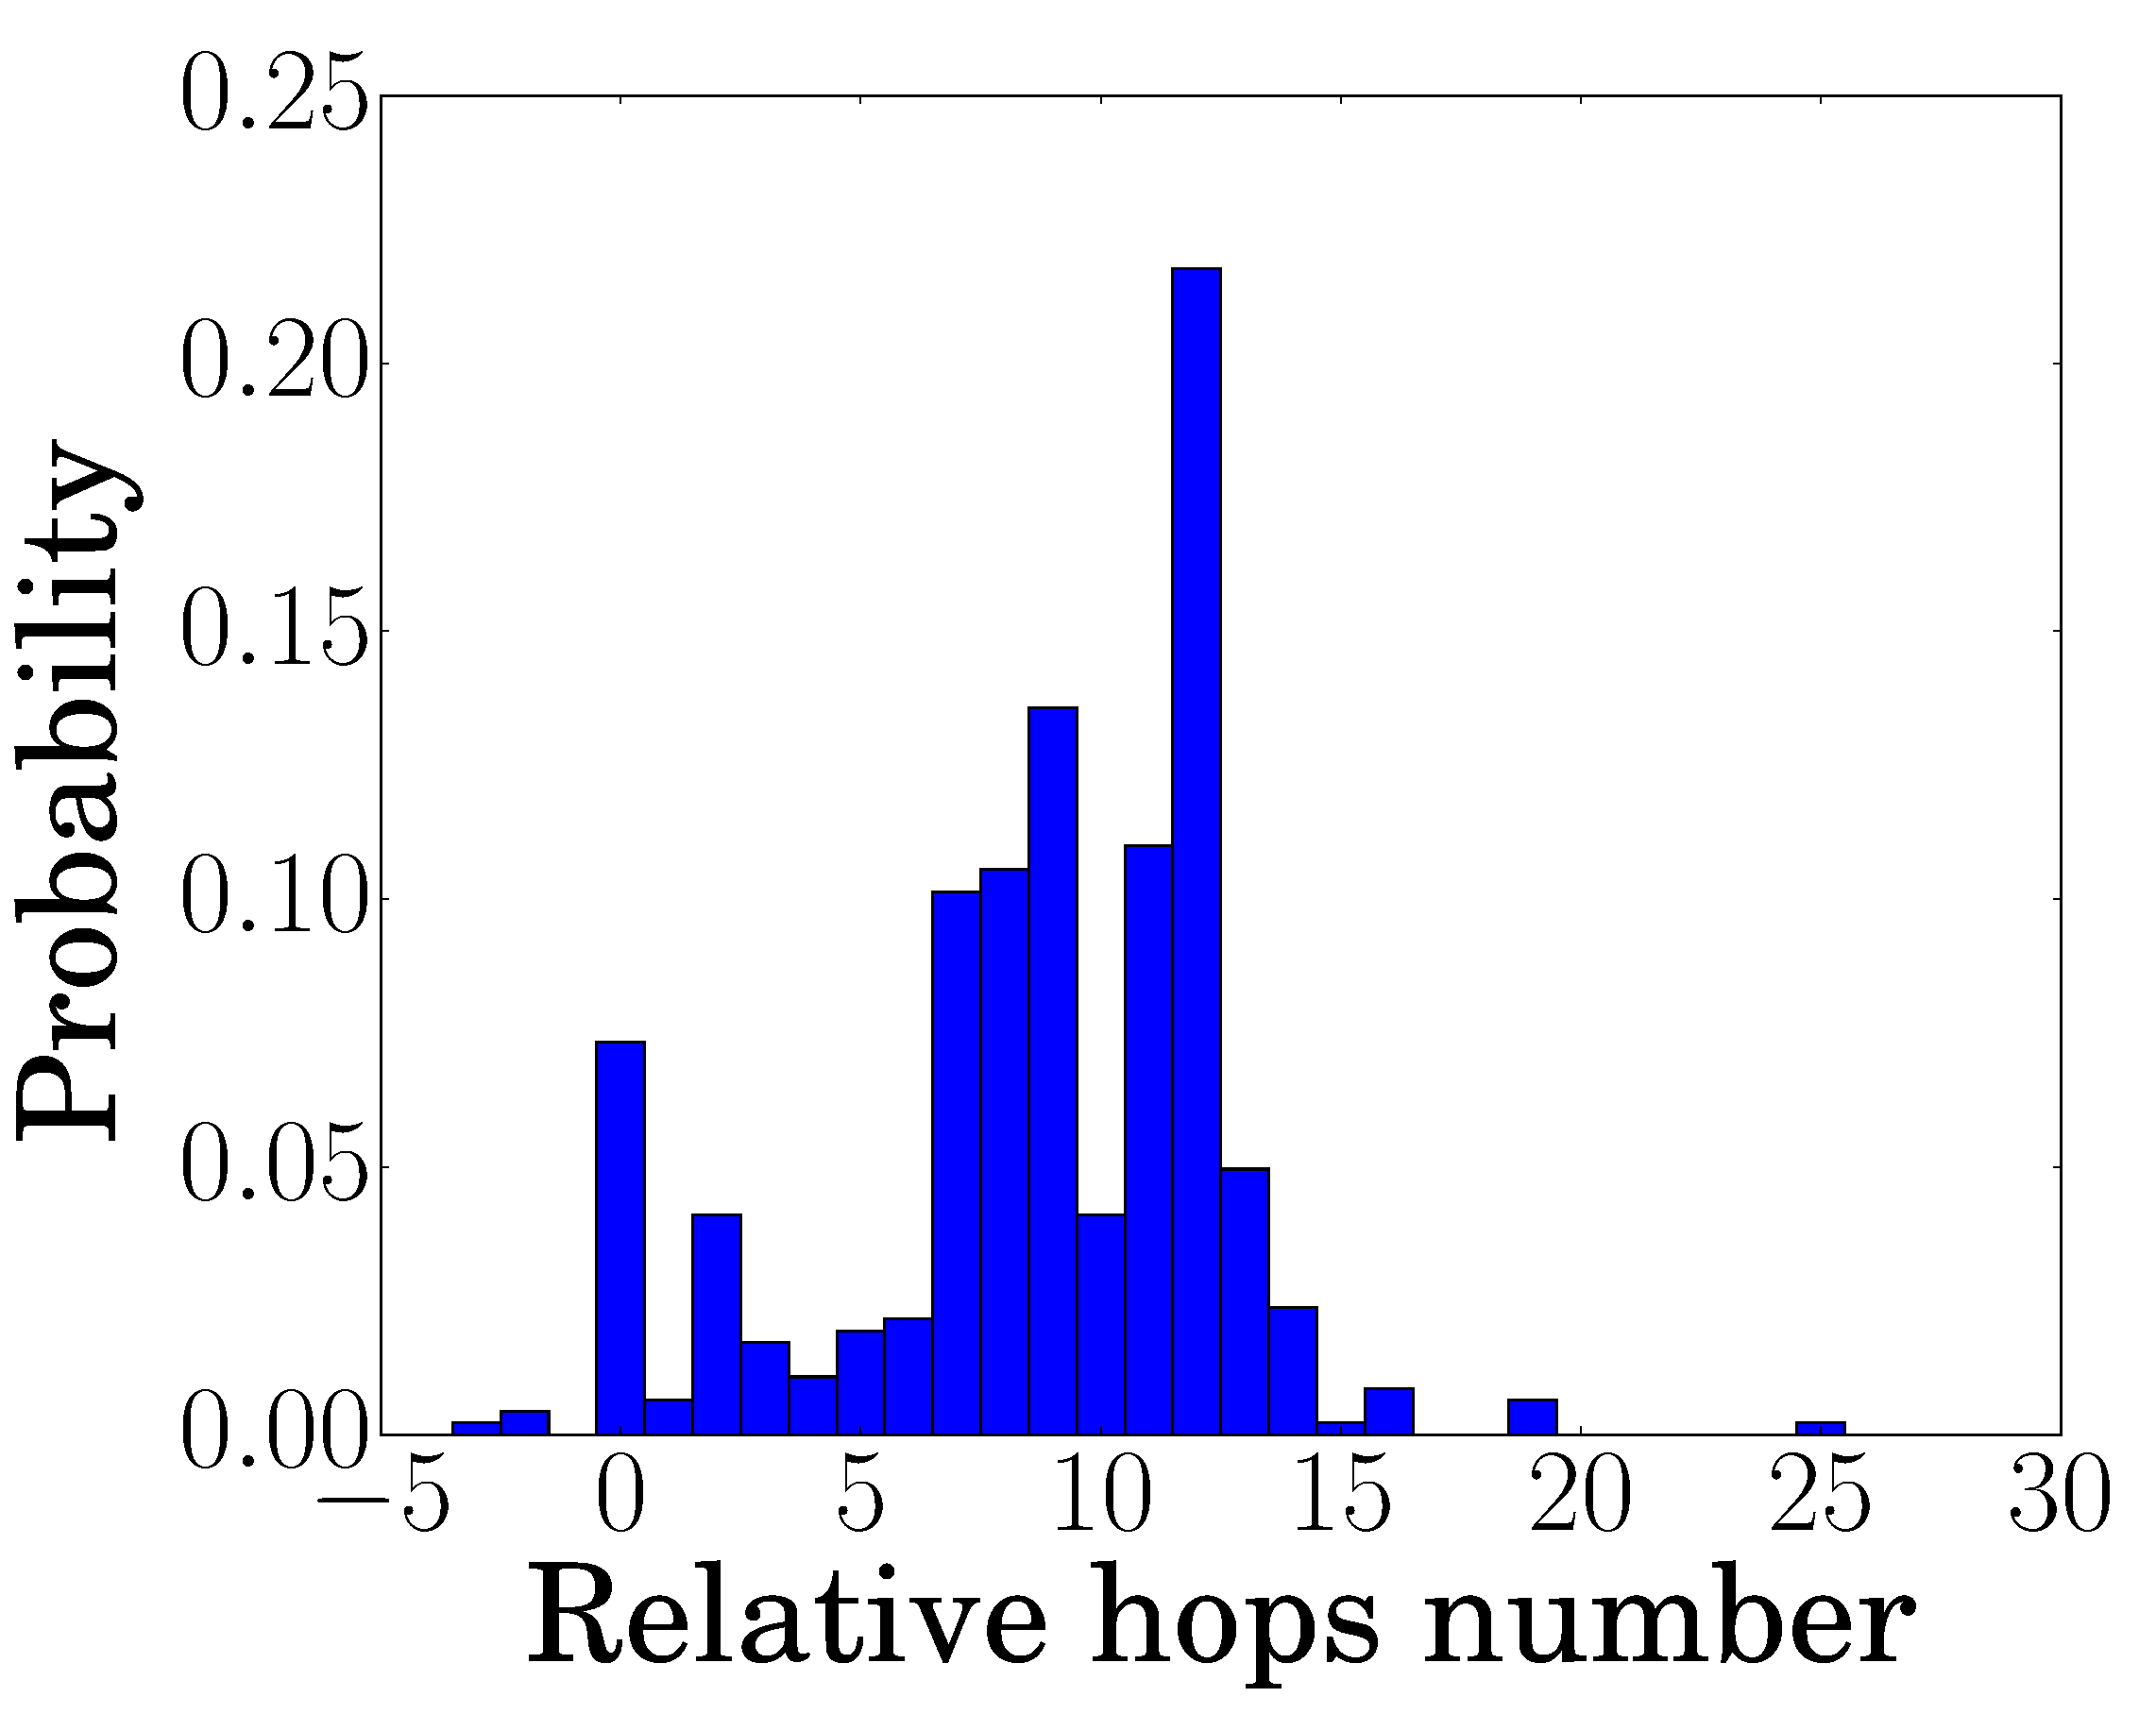
\includegraphics[width=\textwidth]{Pics/v4/Relative_hops_num_LISP-Lab-FranceIX_hist_changed_60.eps}
		\end{center}
	\end{minipage}
	\begin{minipage}[c]{.49\linewidth}
		\begin{center}
			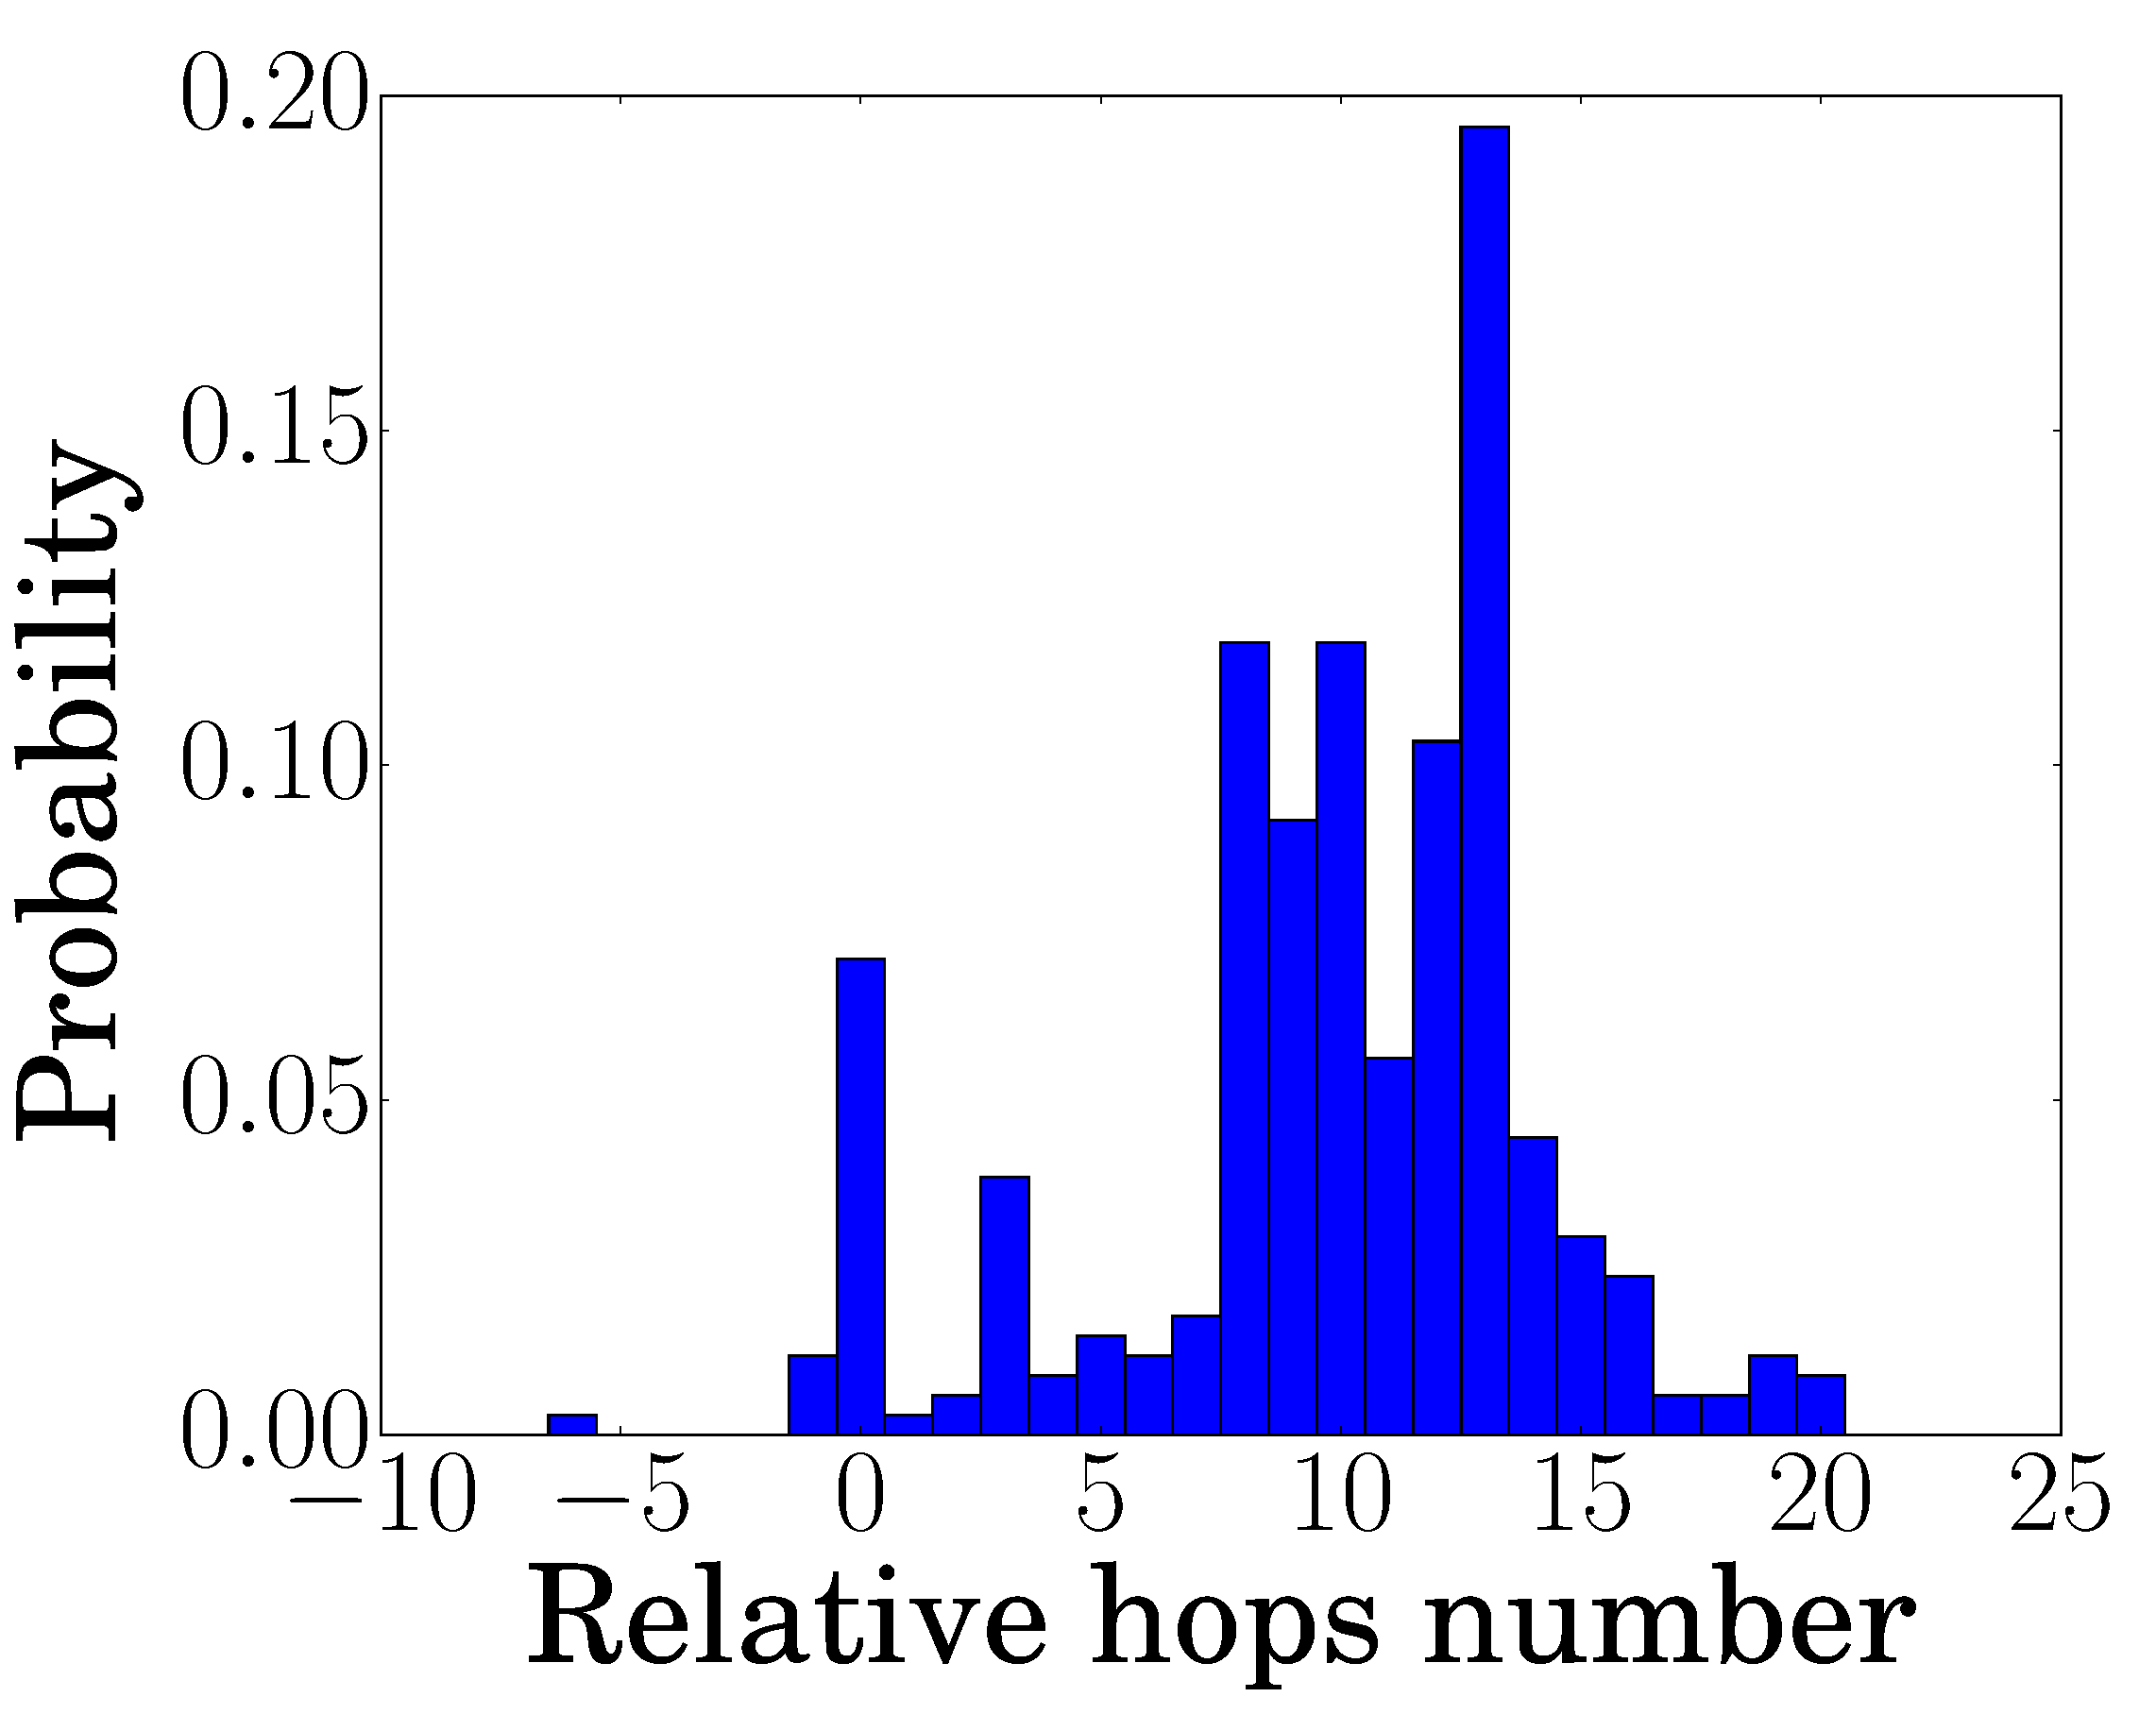
\includegraphics[width=\textwidth]{Pics/v4/Relative_hops_num_LIP6-FranceIX_hist_changed_60.eps}
		\end{center}
	\end{minipage}
	\vspace{-0.5mm}
	\caption{Distribution of IPv4 Relative Hops Number for LISP-Lab (left) and LIP6 (right) from Dataset 2016}
	\label{Distribution_v4_relative_hops_num_proporation_LISP-Lab_LIP6}
\end{figure}
%-< END FIGURE >--------------------------------------------------------------------

As FranceIX is always the most stable probe and has the shortest path in most cases, we define \emph{Relative Hops Number (rHN)} clustered by different continents to look at the difference between the hops number of LISP probes and FranceIX. The definition is as: % $Hops Num_{LISP-Lab}$ - $Hops Num_{FranceIX}$ and $Hops Num_{LIP6}$ - $Hops Num_{FranceIX}$. 
\begin{equation}
    \label{rHN_ll_2016}
    rHN_{LL}(d)=HN_{LL}(d) - HN_{F}(d) 
\end{equation}
\begin{equation}
    \label{rHN_l6_2016}
    rHN_{L6}(d)=HN_{L6}(d) - HN_{F}(d) 
\end{equation}
where $d$ is the destination, subscriptions $LL$, $L6$ and $F$ respectively refers to LISP-Lab, LIP6 and FranceIX. The positive value indicates that the hops number of FranceIX is smaller than LISP probes. Fig.~\ref{Distribution_v4_relative_hops_num_proporation_LISP-Lab_LIP6} provides an IPv4 distribution of relative hops number for LISP-Lab on the left and for LIP6 on the right. This figure shows the probability of each relative hops number. For the LISP-Lab probe, the most common relative hops number is 12 with a percentage of $21.77\%$, hence remaining limited in most of the cases. From the ping-related experiment in Sec.~\ref{sec:pxtr_ping_v4_2016} and Sec.~\ref{sec:pxtr_ping_v6} we know that using PxTR introduces some overhead. So the Relative Hops Number being generally positive is reasonable. The very large relative hops number just appears once for 19 and 25, so we regard them as outliers. Similar to the LISP-Lab case, for the LIP6 probe, the most frequent relative hops number is 13 in $19.53\%$ of cases.

%-< FIGURE >--------------------------------------------------------------------
\begin{figure}[!t]
	\begin{minipage}[c]{.49\linewidth}
		\begin{center}
			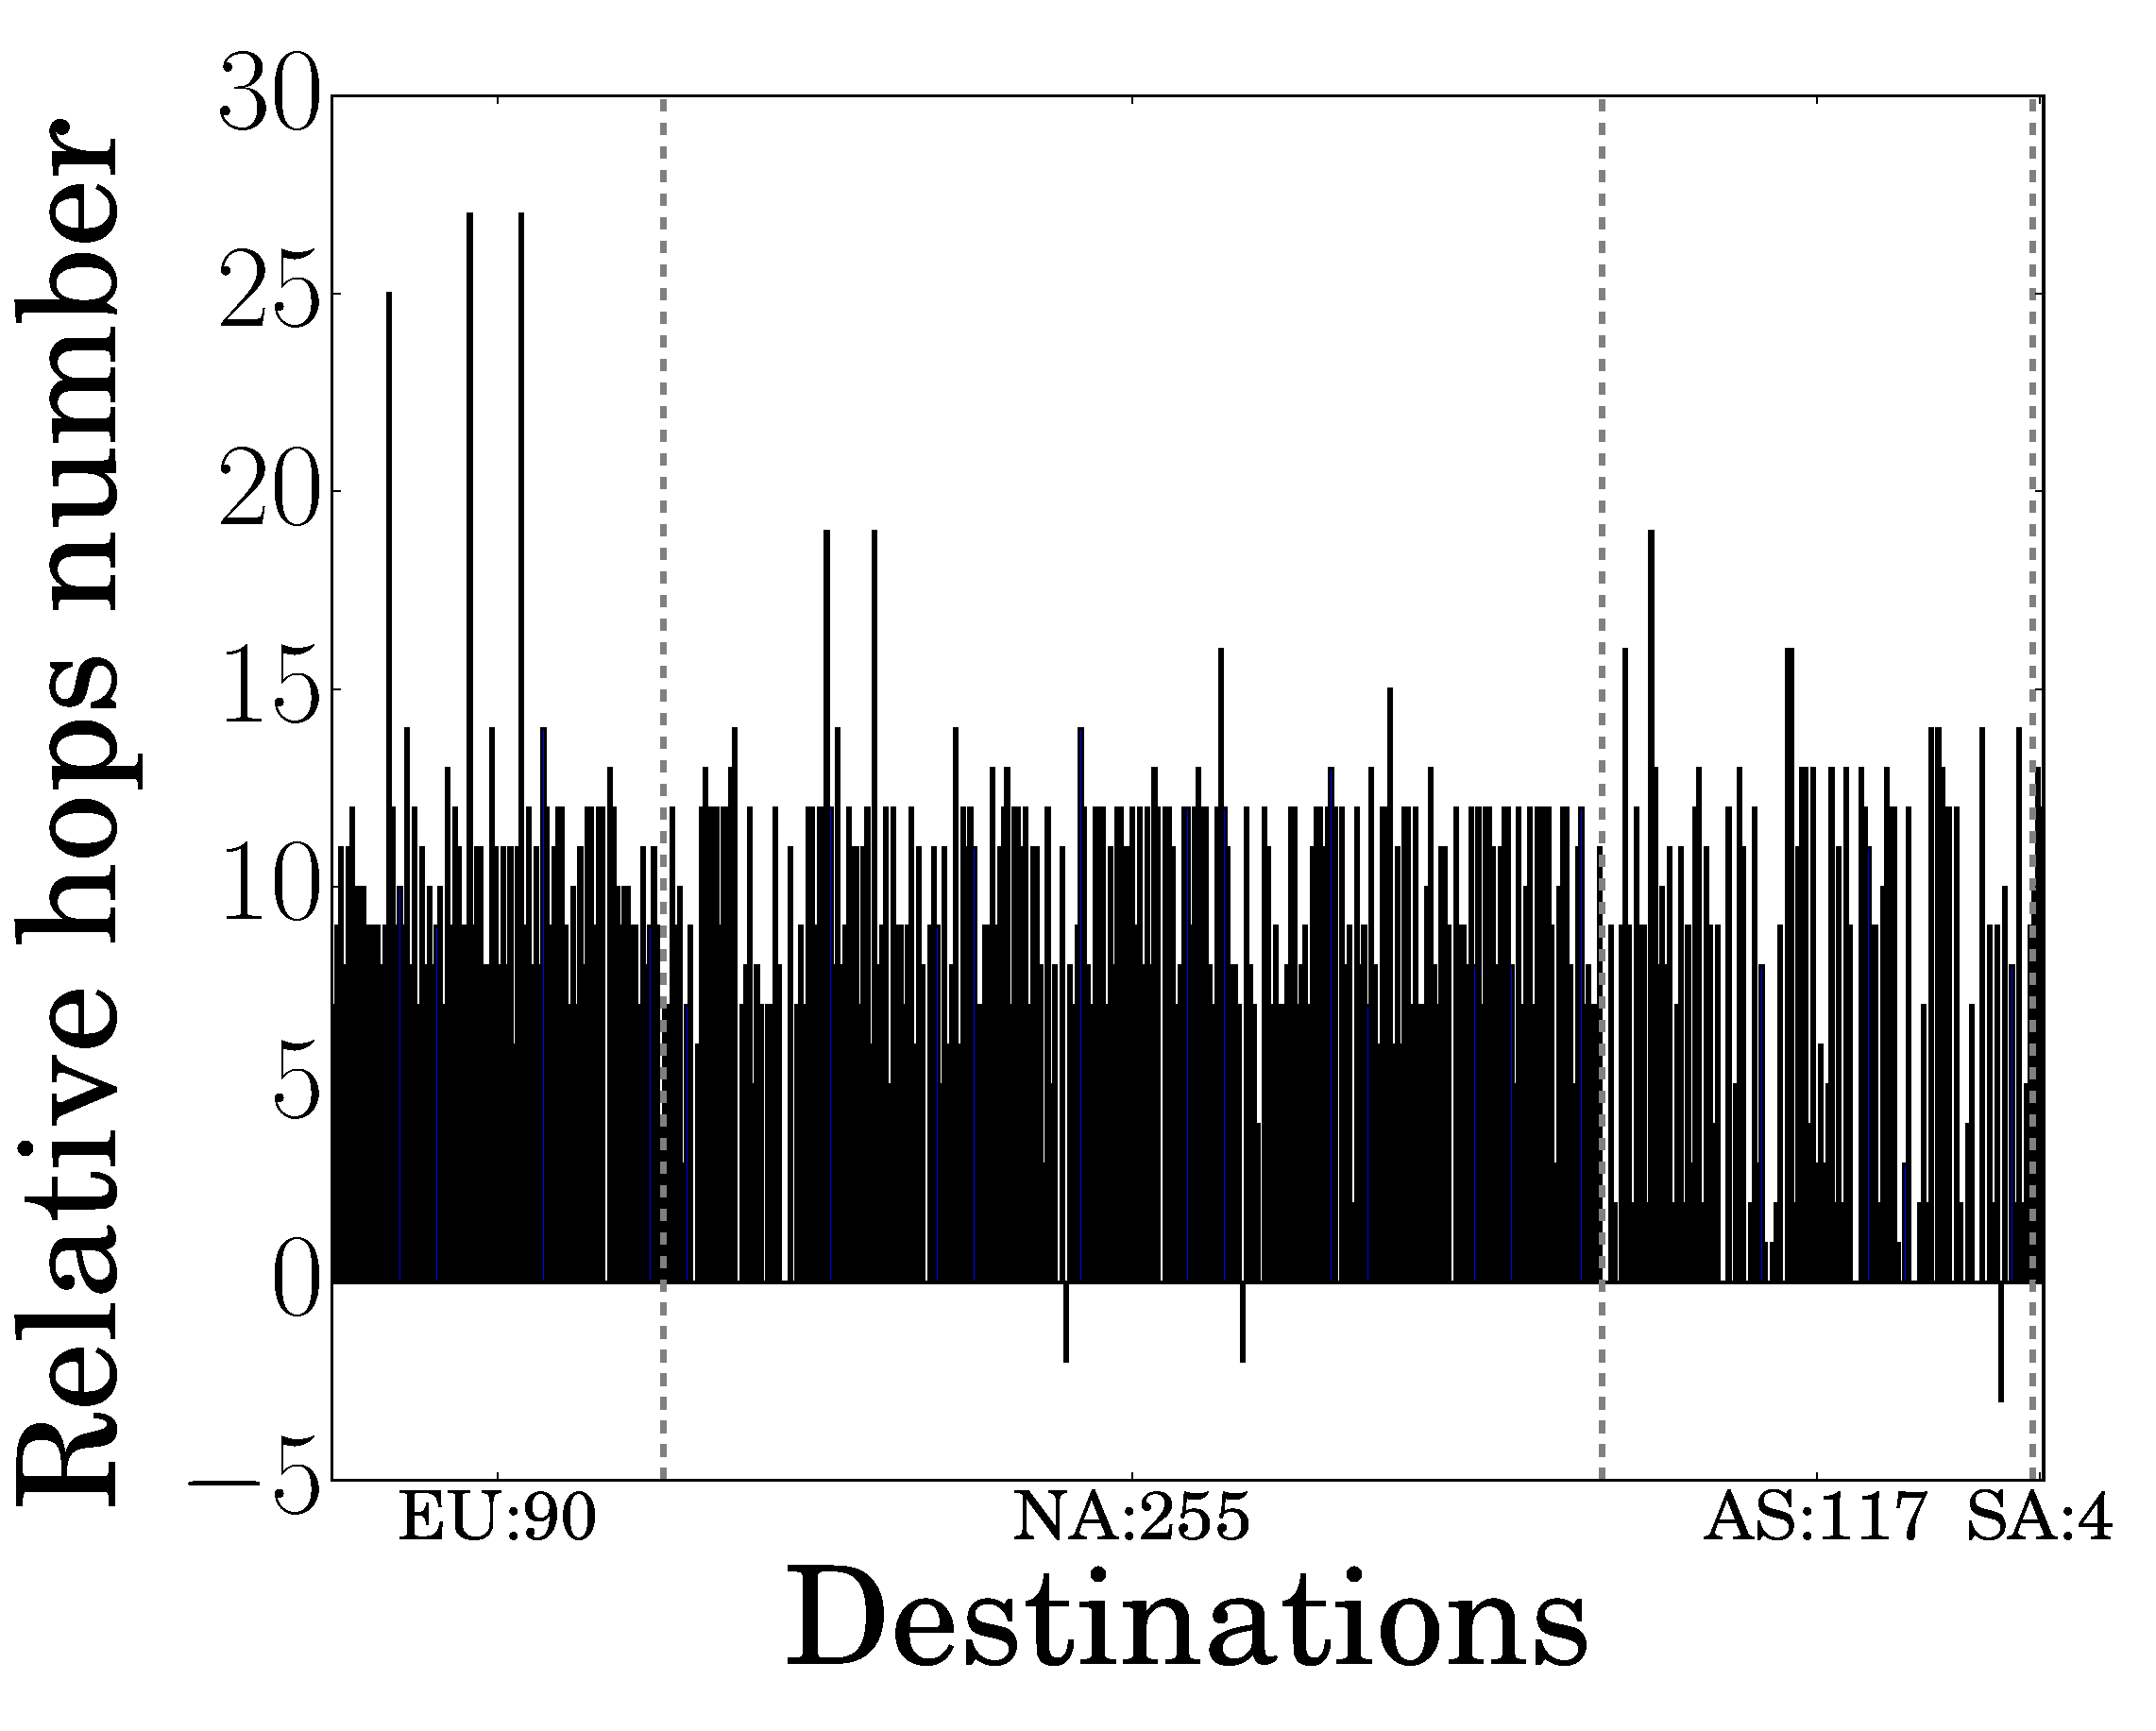
\includegraphics[width=\textwidth]{Pics/v4/Relative_hops_num_LISP-Lab-FranceIX_changed_60.eps}
		\end{center}
	\end{minipage}
	\begin{minipage}[c]{.49\linewidth}
		\begin{center}
			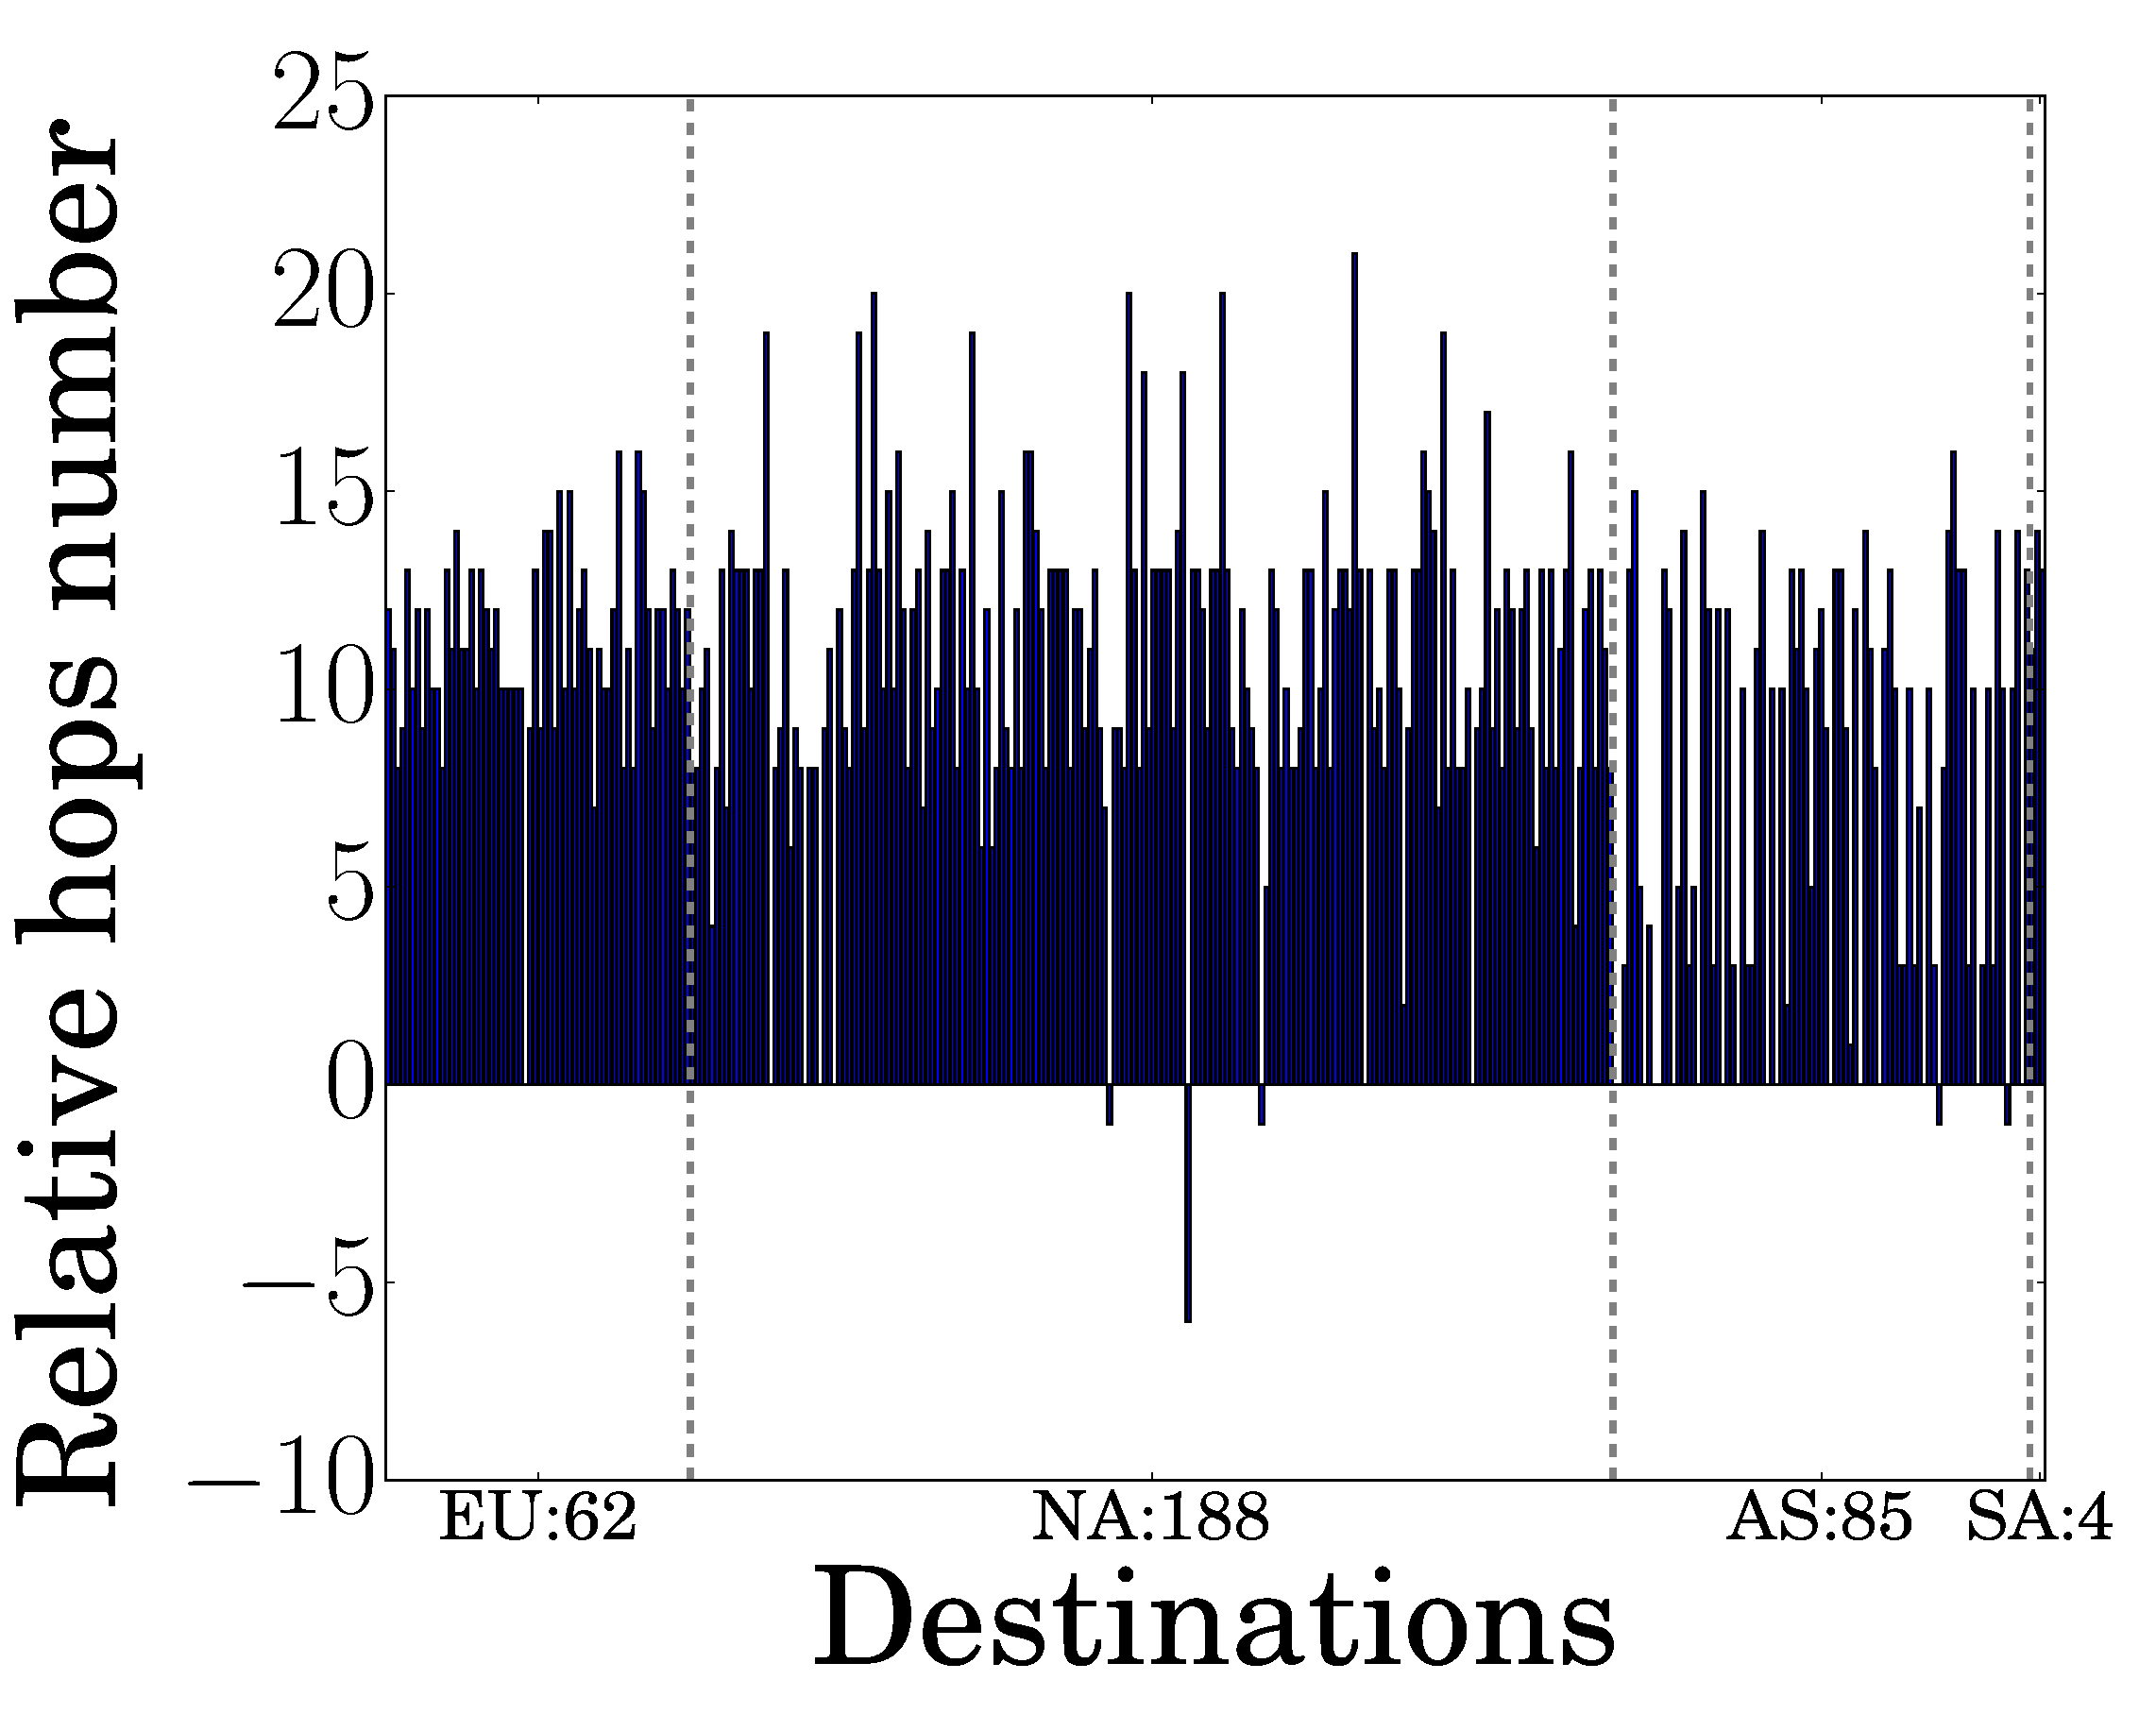
\includegraphics[width=\textwidth]{Pics/v4/Relative_hops_num_LIP6-FranceIX_changed_60.eps}
		\end{center}
	\end{minipage}
	\vspace{-0.5mm}
	\caption{IPv4 Relative hops number clustered by different continents for LISP-Lab (left) and LIP6 (right) from Dataset 2016}
	\label{v4_Relative_hops_num}
\end{figure}
%-< END FIGURE >--------------------------------------------------------------------

In order to understand where the most common relative hops number appears, we produce the relative hops number for each destination clustered by different continents in Fig.~\ref{v4_Relative_hops_num} to complete Fig.~\ref{Distribution_v4_relative_hops_num_proporation_LISP-Lab_LIP6}. The left figure is for the LISP-Lab probe, indicating that the relative hops number is almost the same for the European and North American destinations and contributes to the relative hops number with high probabilities in Fig.~\ref{Distribution_v4_relative_hops_num_proporation_LISP-Lab_LIP6}. The small relative hops number is mostly produced from the Asian targets. Whereas the outliers are all from the European destinations. The right figure of Fig.~\ref{v4_Relative_hops_num} is for the LIP6 probe, mainly presenting the same result as the LISP-Lab probe, except that the latter rarely has the relative hops number higher than 16, but LIP6 has more.

%-< FIGURE >--------------------------------------------------------------------
\begin{figure}[!t]
	\begin{minipage}[c]{.49\linewidth}
		\begin{center}
			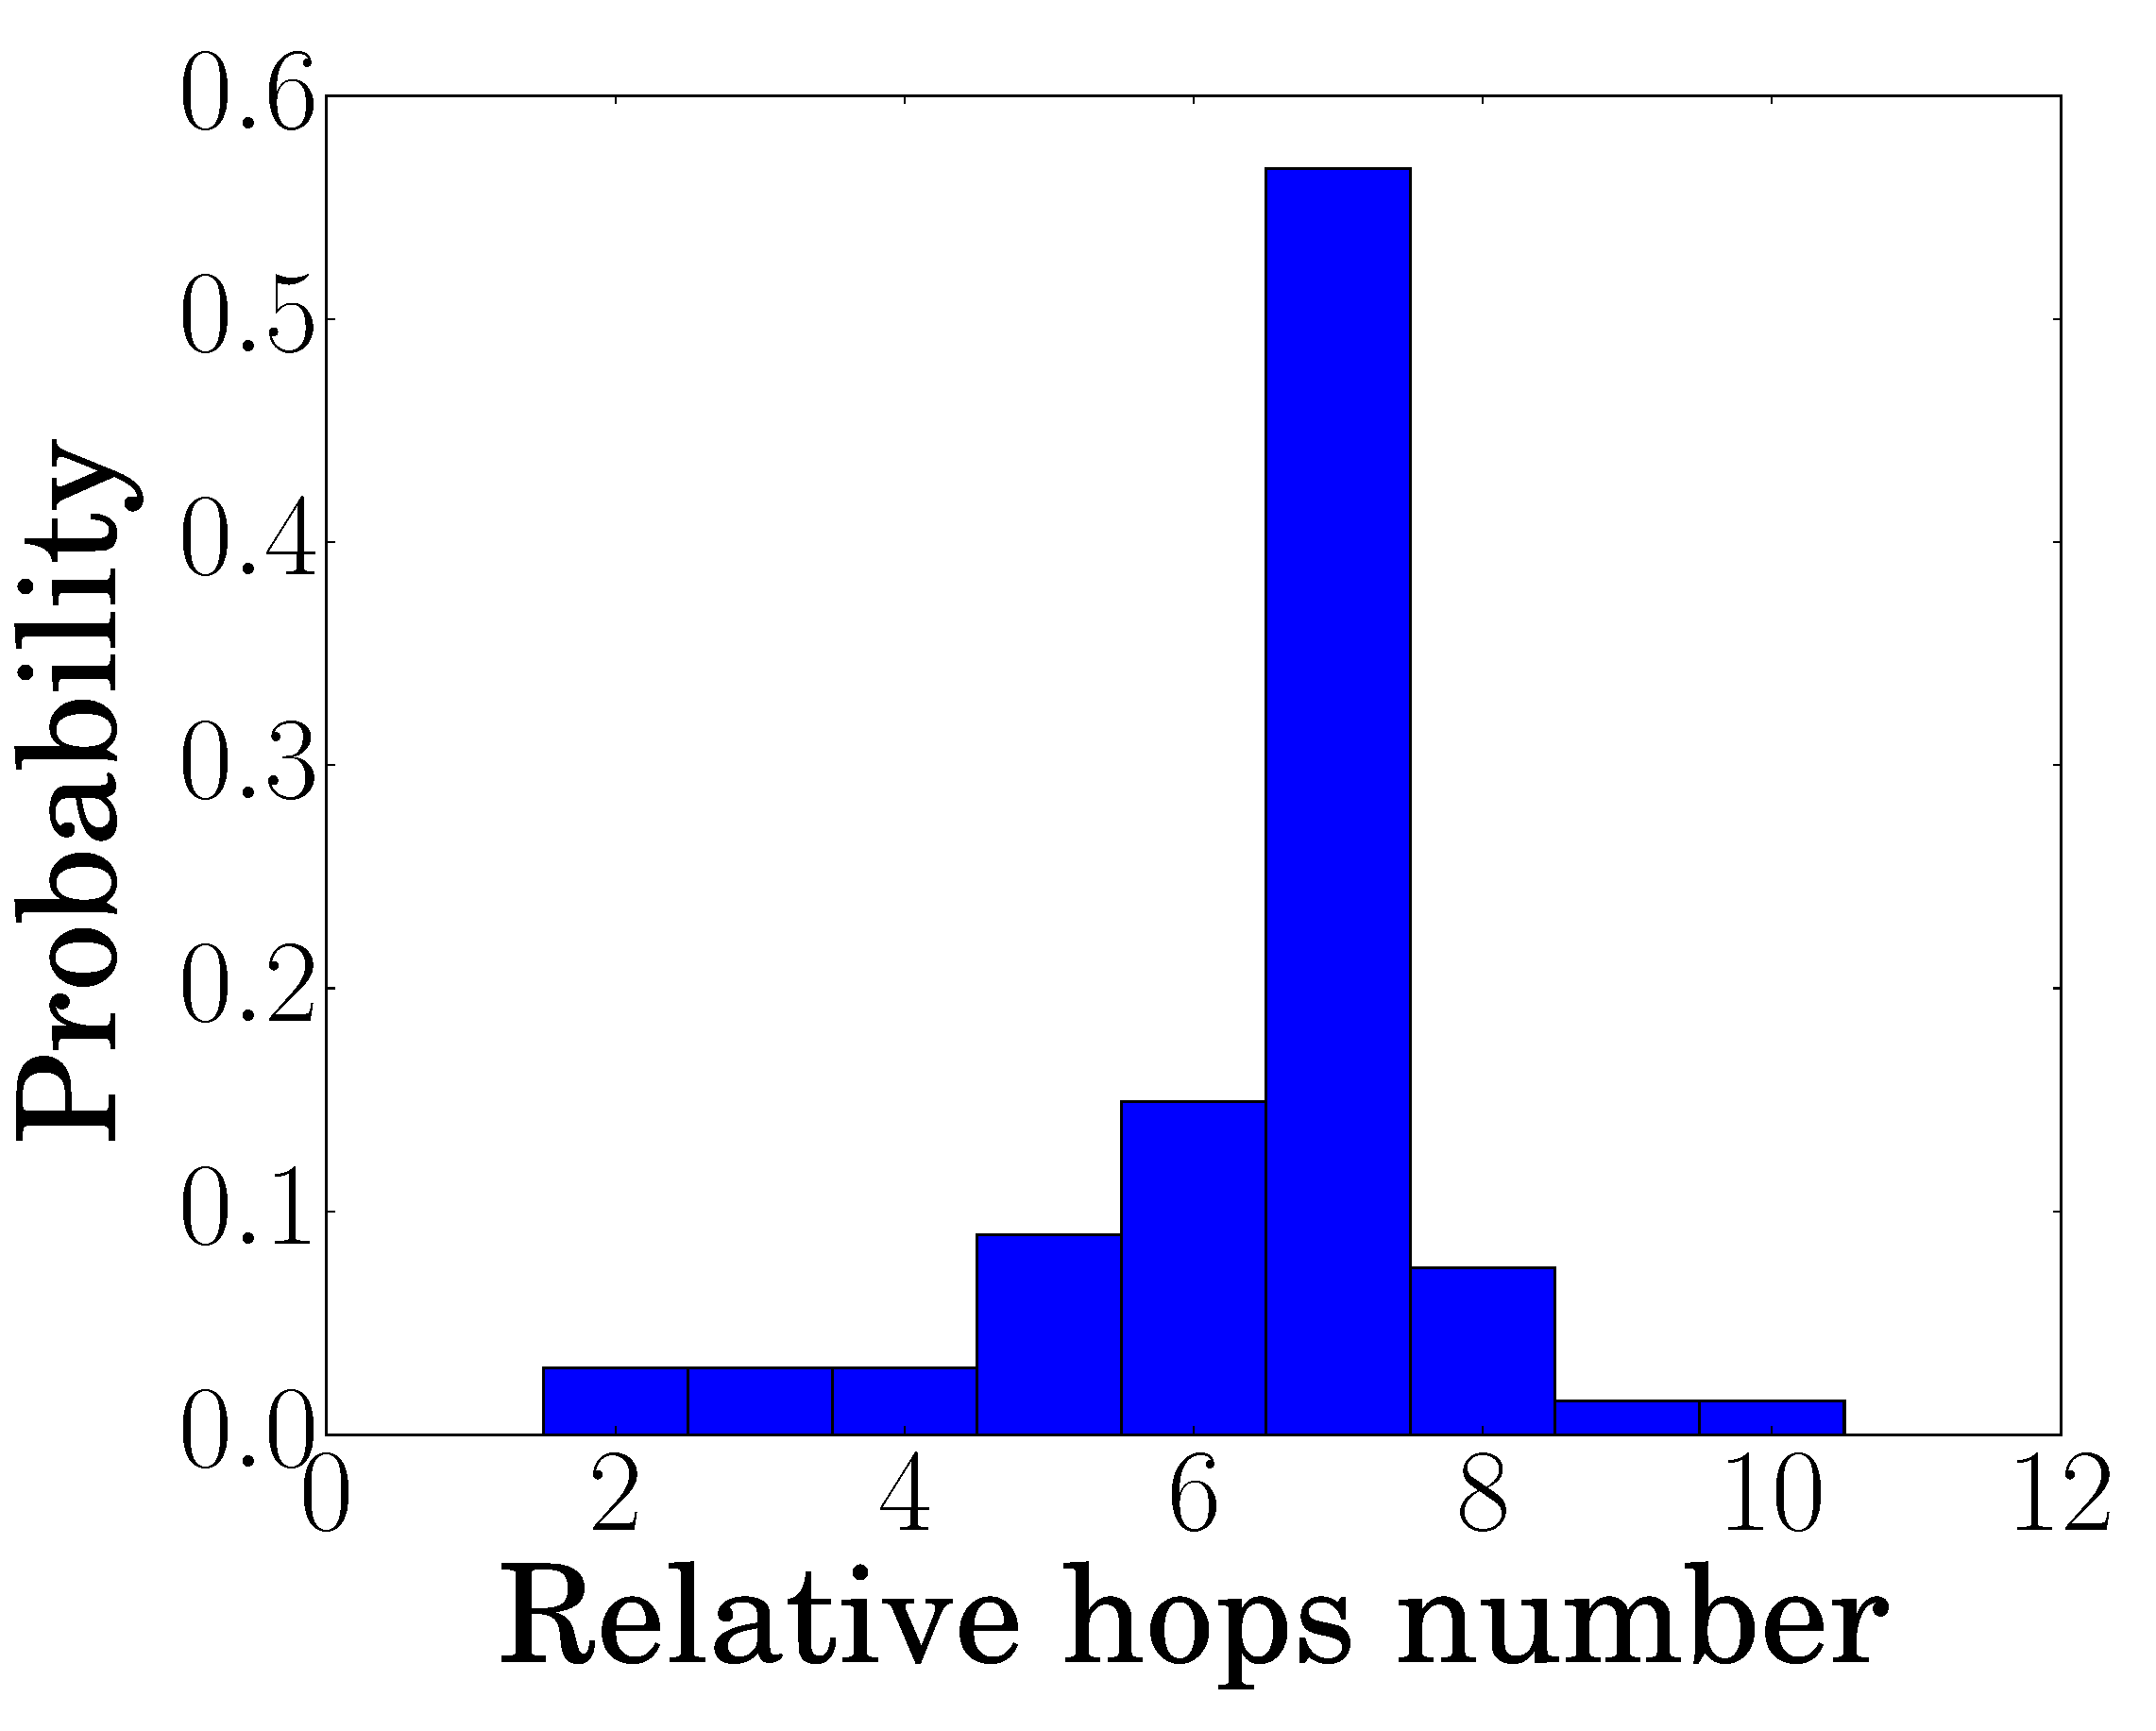
\includegraphics[width=\textwidth]{Pics/v6/Relative_hops_num_LISP-Lab-FranceIX_hist_changed_60.eps}
		\end{center}
	\end{minipage}
	\begin{minipage}[c]{.49\linewidth}
		\begin{center}
			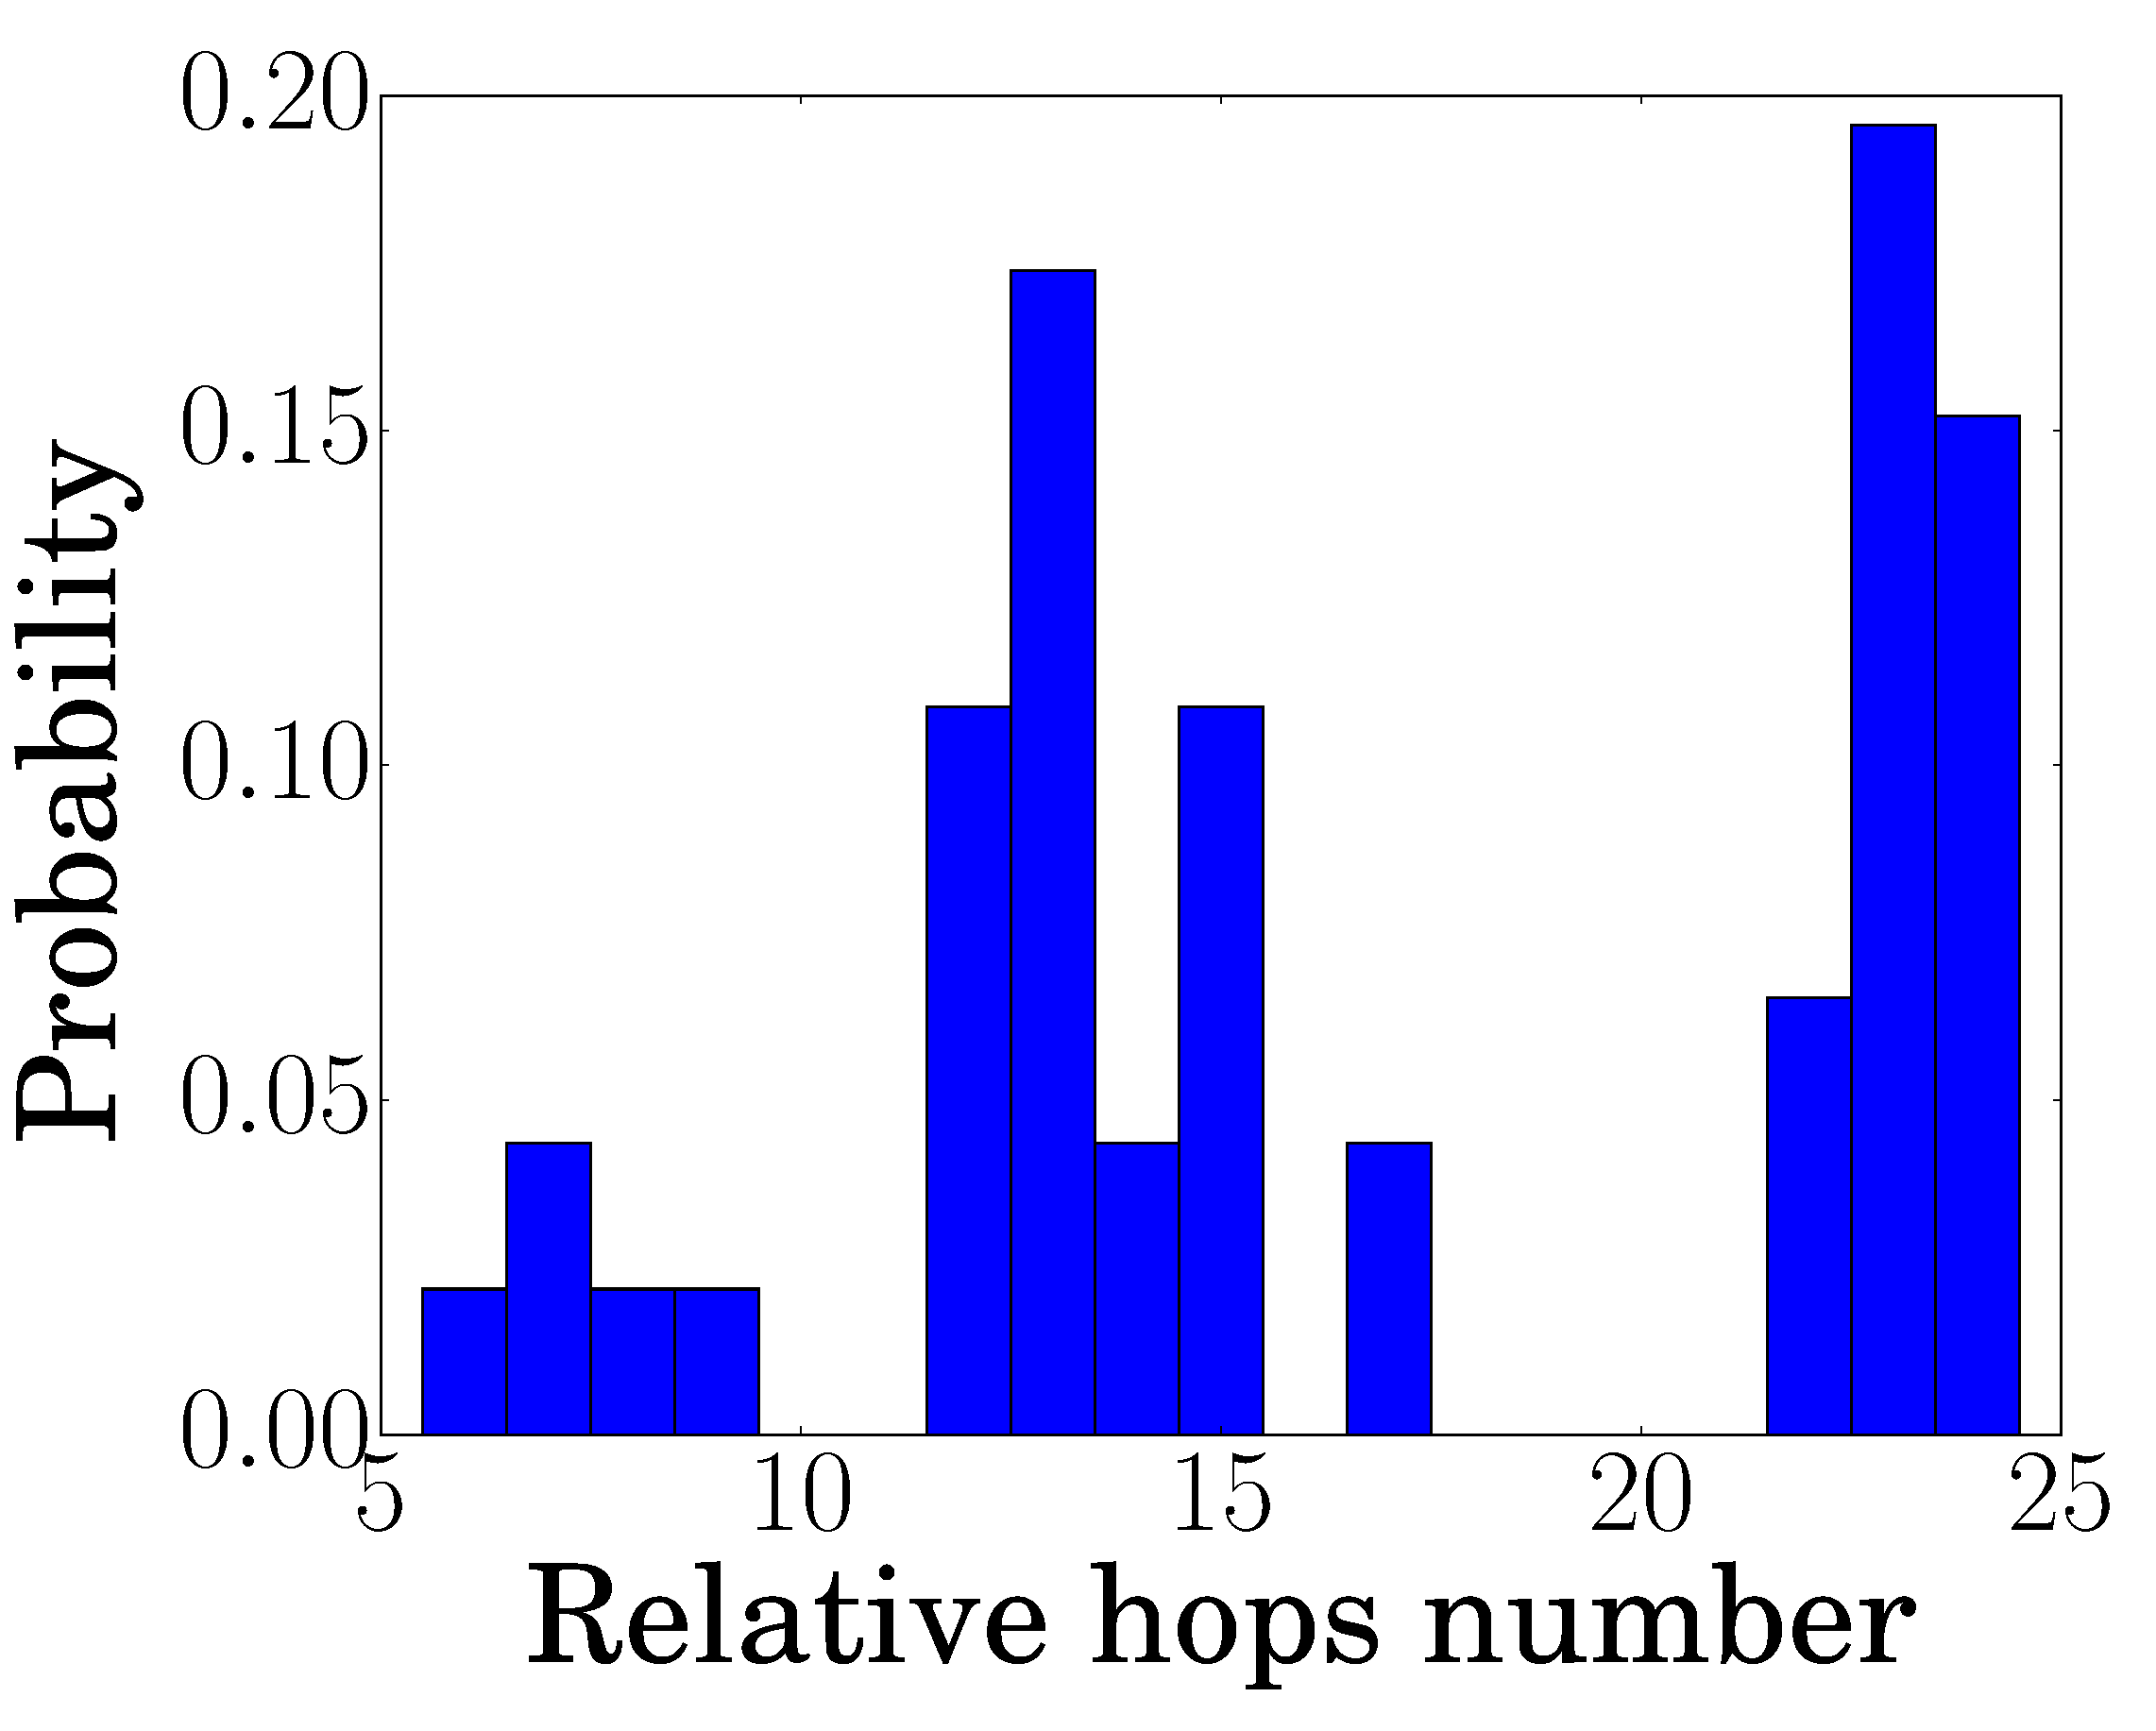
\includegraphics[width=\textwidth]{Pics/v6/Relative_hops_num_LIP6-FranceIX_hist_changed_60.eps}
		\end{center}
	\end{minipage}
	\vspace{-0.5mm}
	\caption{Distribution of IPv6 Relative Hops Number for LISP-Lab (left) and LIP6 (right) from Dataset 2016}
	\label{Distribution_v6_relative_hops_num_proporation_LISP-Lab_LIP6}
\end{figure}
%-< END FIGURE >--------------------------------------------------------------------

With the same evaluation metrics of IPv4, the distribution of Relative Hops Number and the Relative Hops Number clustered by different continents for IPv6 are respectively shown in Fig.~\ref{Distribution_v6_relative_hops_num_proporation_LISP-Lab_LIP6} and Fig.~\ref{v6_Relative_hops_num}. The left figure of Fig.~\ref{Distribution_v6_relative_hops_num_proporation_LISP-Lab_LIP6} presents that the most common relative hops number between the FranceIX anchor and the LISP-Lab probe is 7 in $56.72\%$ of cases, more than a half, much higher than the probability of other relative hops numbers. The range of relative hops number is smaller compared to IPv4 and the most common relative hops number is also smaller, since the traffic does not need to pass the PETR, but is just natively forwarded so the overhead is reduced. The left figure of Fig.~\ref{v6_Relative_hops_num} reveals the truth that 7 relative hops numbers are produced by the majority of targets regardless where the destinations are, instead of like the one of IPv4, where the relative hops number for European and American destinations are more than the Asian's. As the relative hops number from PETR is only 3, but 7 for natively forwarding, it is likely that the PxTR has shorter paths to most destinations, leads to the decreasing of hops number for the LISP-Lab probe. The relative RTTs higher for European and American destinations than those for Asia shown in left figure of Fig.~\ref{Relative_median_avg(RTT)_v6_2016} are mainly caused by the returning path, since it is natively forward for outgoing and there is no difference by continents. For IPv6, the LIP6 probe has extremely high relative hops number in a range from 12 to 24. The majority of relative hops number is 23 in $19.57\%$ of the cases and followed by 13 with a percentage of $17.39\%$. The higher relative hops number is caused by not using the VPN between xTR and PETR compared to the IPv4 case. The right figure of Fig.~\ref{v6_Relative_hops_num} visualizes the 23 relative hops number coming from the European destinations and 13 coming from the Asian targets. The form coincides to the relative RTT for IPv6 shown in the right hand part of Fig.~\ref{Relative_median_avg(RTT)_v6_2016}, indicating that the high relative RTTs are caused by the high relative hops number. 

Concerning the RTT performance of the LISP-Lab probe to Asian destinations, which sometimes shows even better than FranceIX, we analyze the AS-path (Autonomous System path) from FranceIX and LISP-Lab to Asian destinations that the packets traverse. Since all the IPv4 packets from LISP-Lab probe are sent to PETR at Lyon first, so the AS-path discussed in the followings is actually from PETR to the Asian destinations. By comparing the AS-path, we find that FranceIX and LISP-Lab very often take different paths, with only the last 1 or 2 hops in common. Even further, by looking at the geographic location of each hop of \emph{traceroute}, it can be observed that FranceIX and LISP-Lab take the path even in the different directions in most of the cases. In particular, there are 11 destinations out of 117 in total (i.e., 9.4\%) for which the packets sent by LISP-Lab pass through US, while the packets sent by FranceIX pass through Eastern Europe. There are 68 destinations (i.e., 58.1\%), which show exatly the opposite situation, i.e., packets sent by FranceIX pass through US, while packets sent by LISP-Lab pass through Eastern Europe. This last case is when LISP-Lab has smaller RTT (compared to FranceIX), almost all of the times (with only few exceptions). 

%-< FIGURE >--------------------------------------------------------------------
\begin{figure}[!t]
	\begin{minipage}[c]{.49\linewidth}
		\begin{center}
			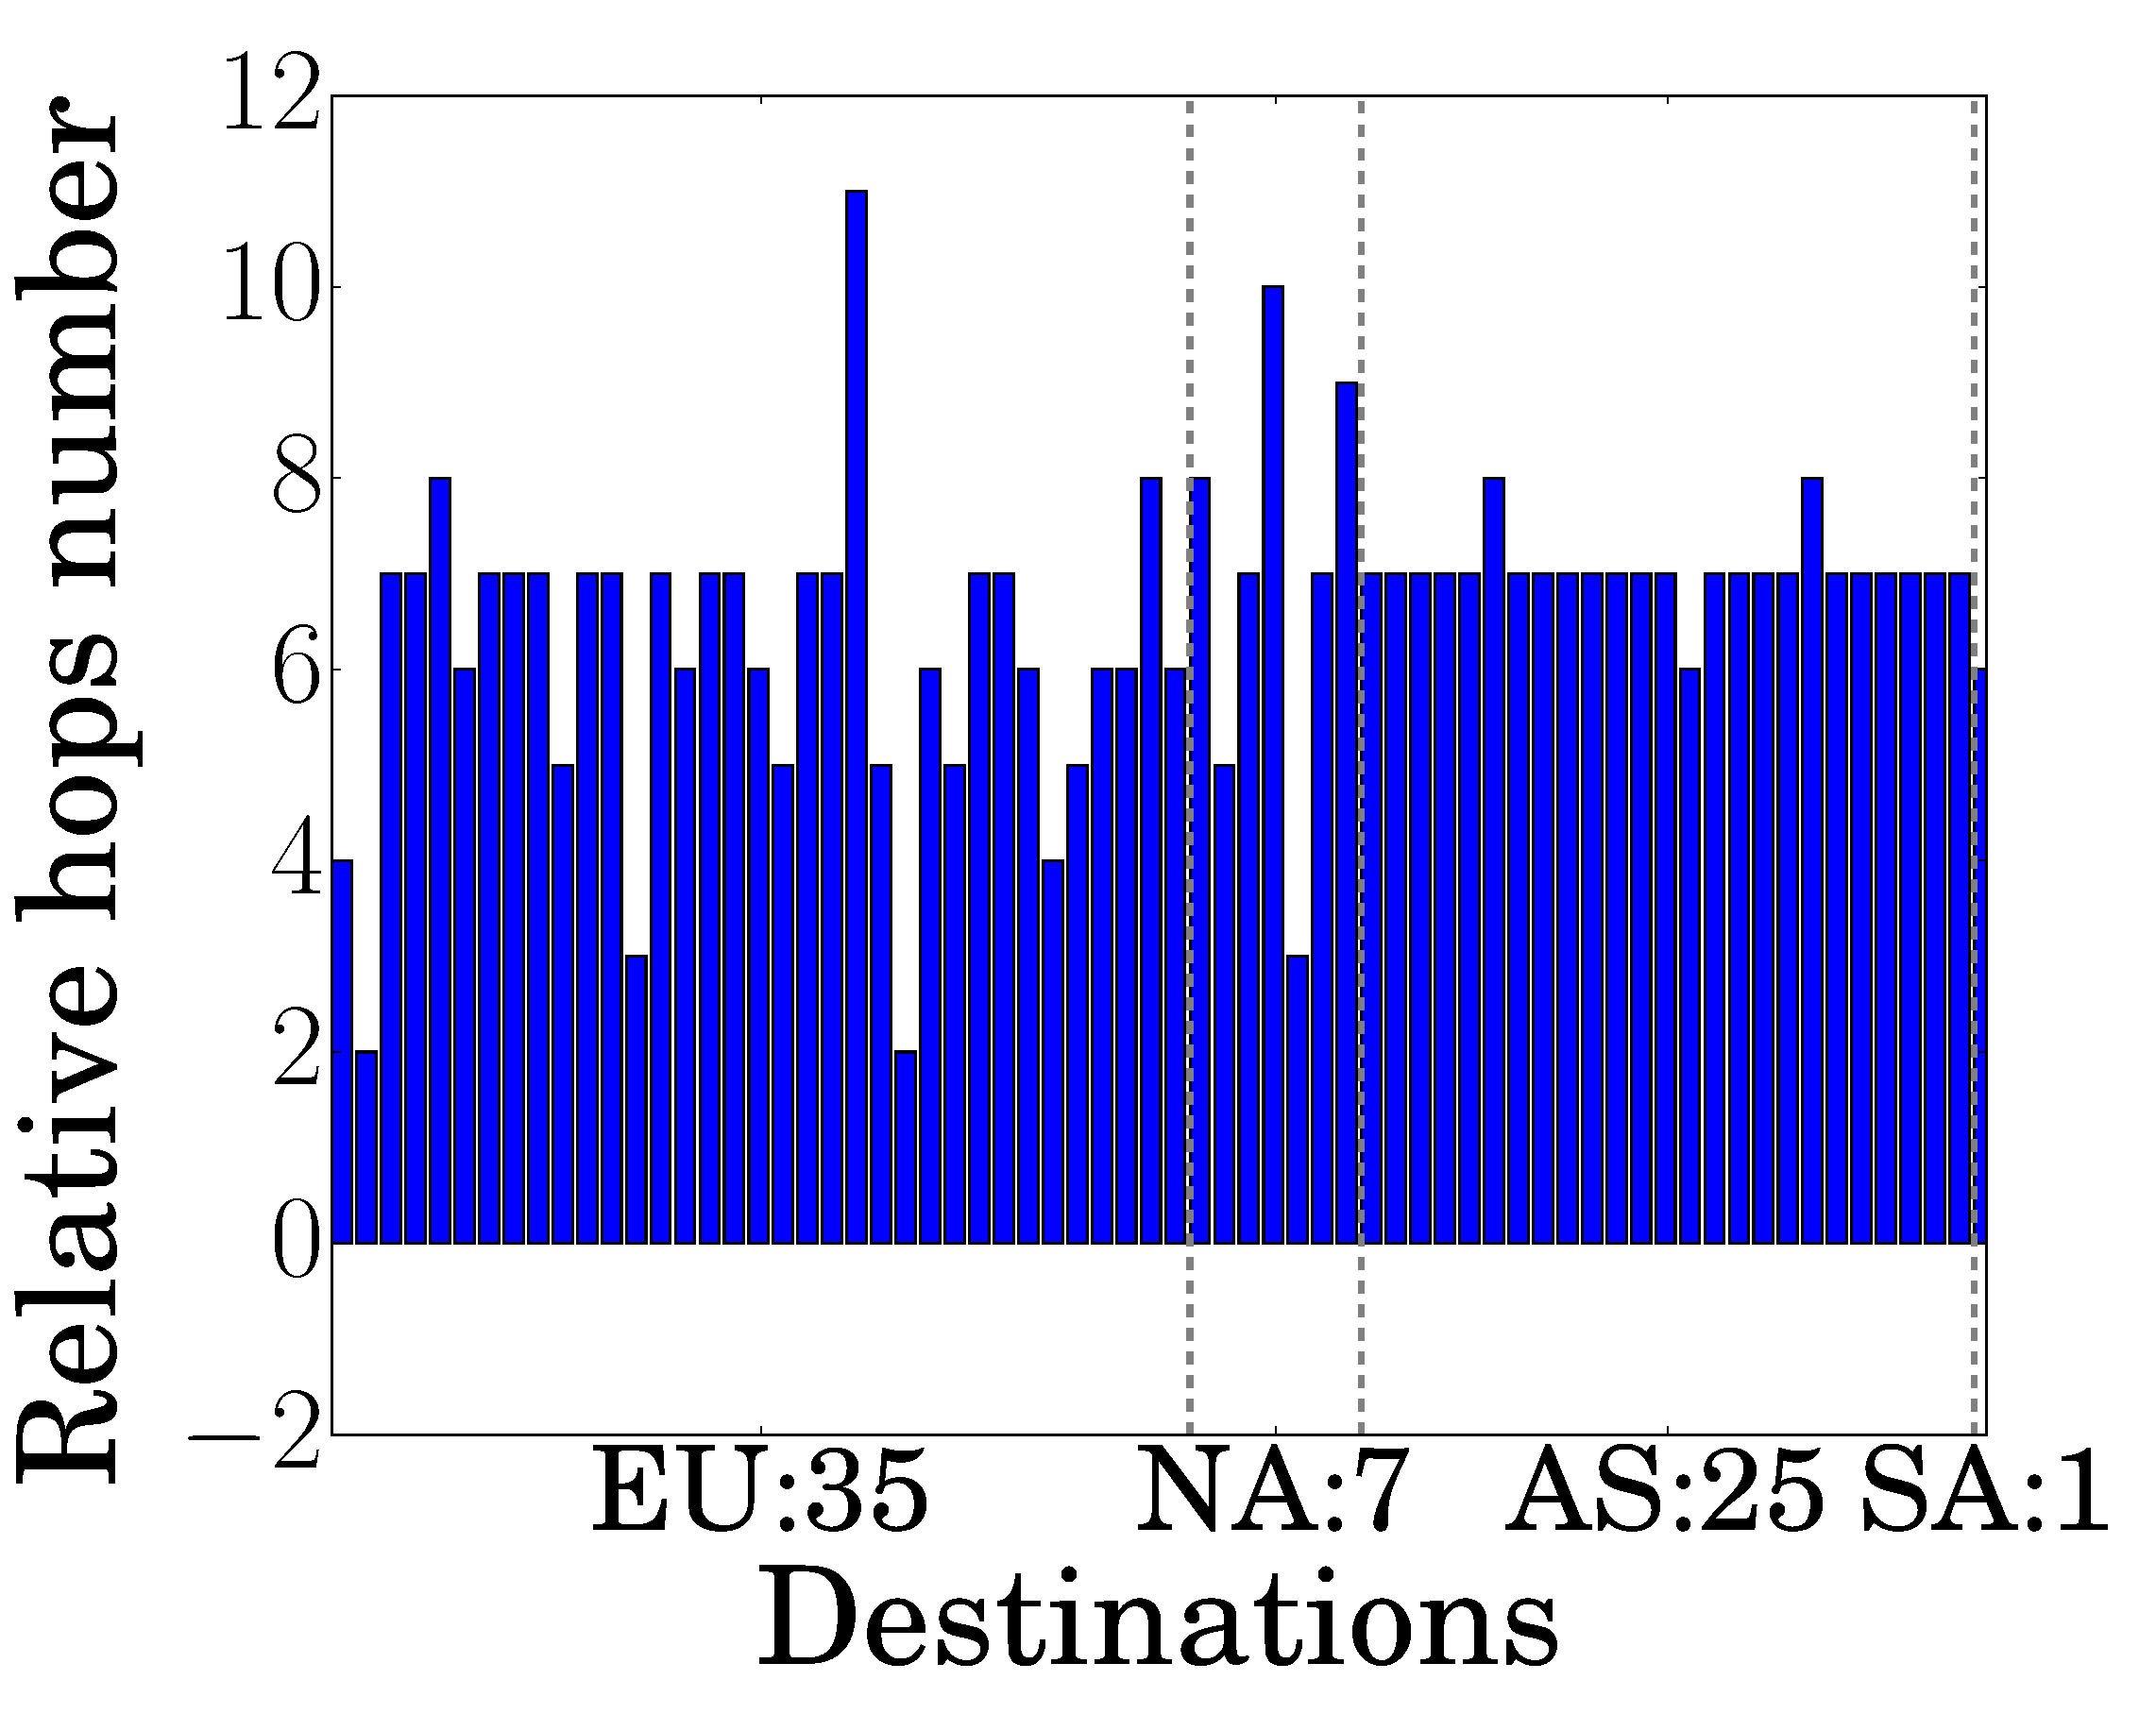
\includegraphics[width=\textwidth]{Pics/v6/Relative_hops_num_LISP-Lab-FranceIX_changed_60.eps}
		\end{center}
	\end{minipage}
	\begin{minipage}[c]{.49\linewidth}
		\begin{center}
			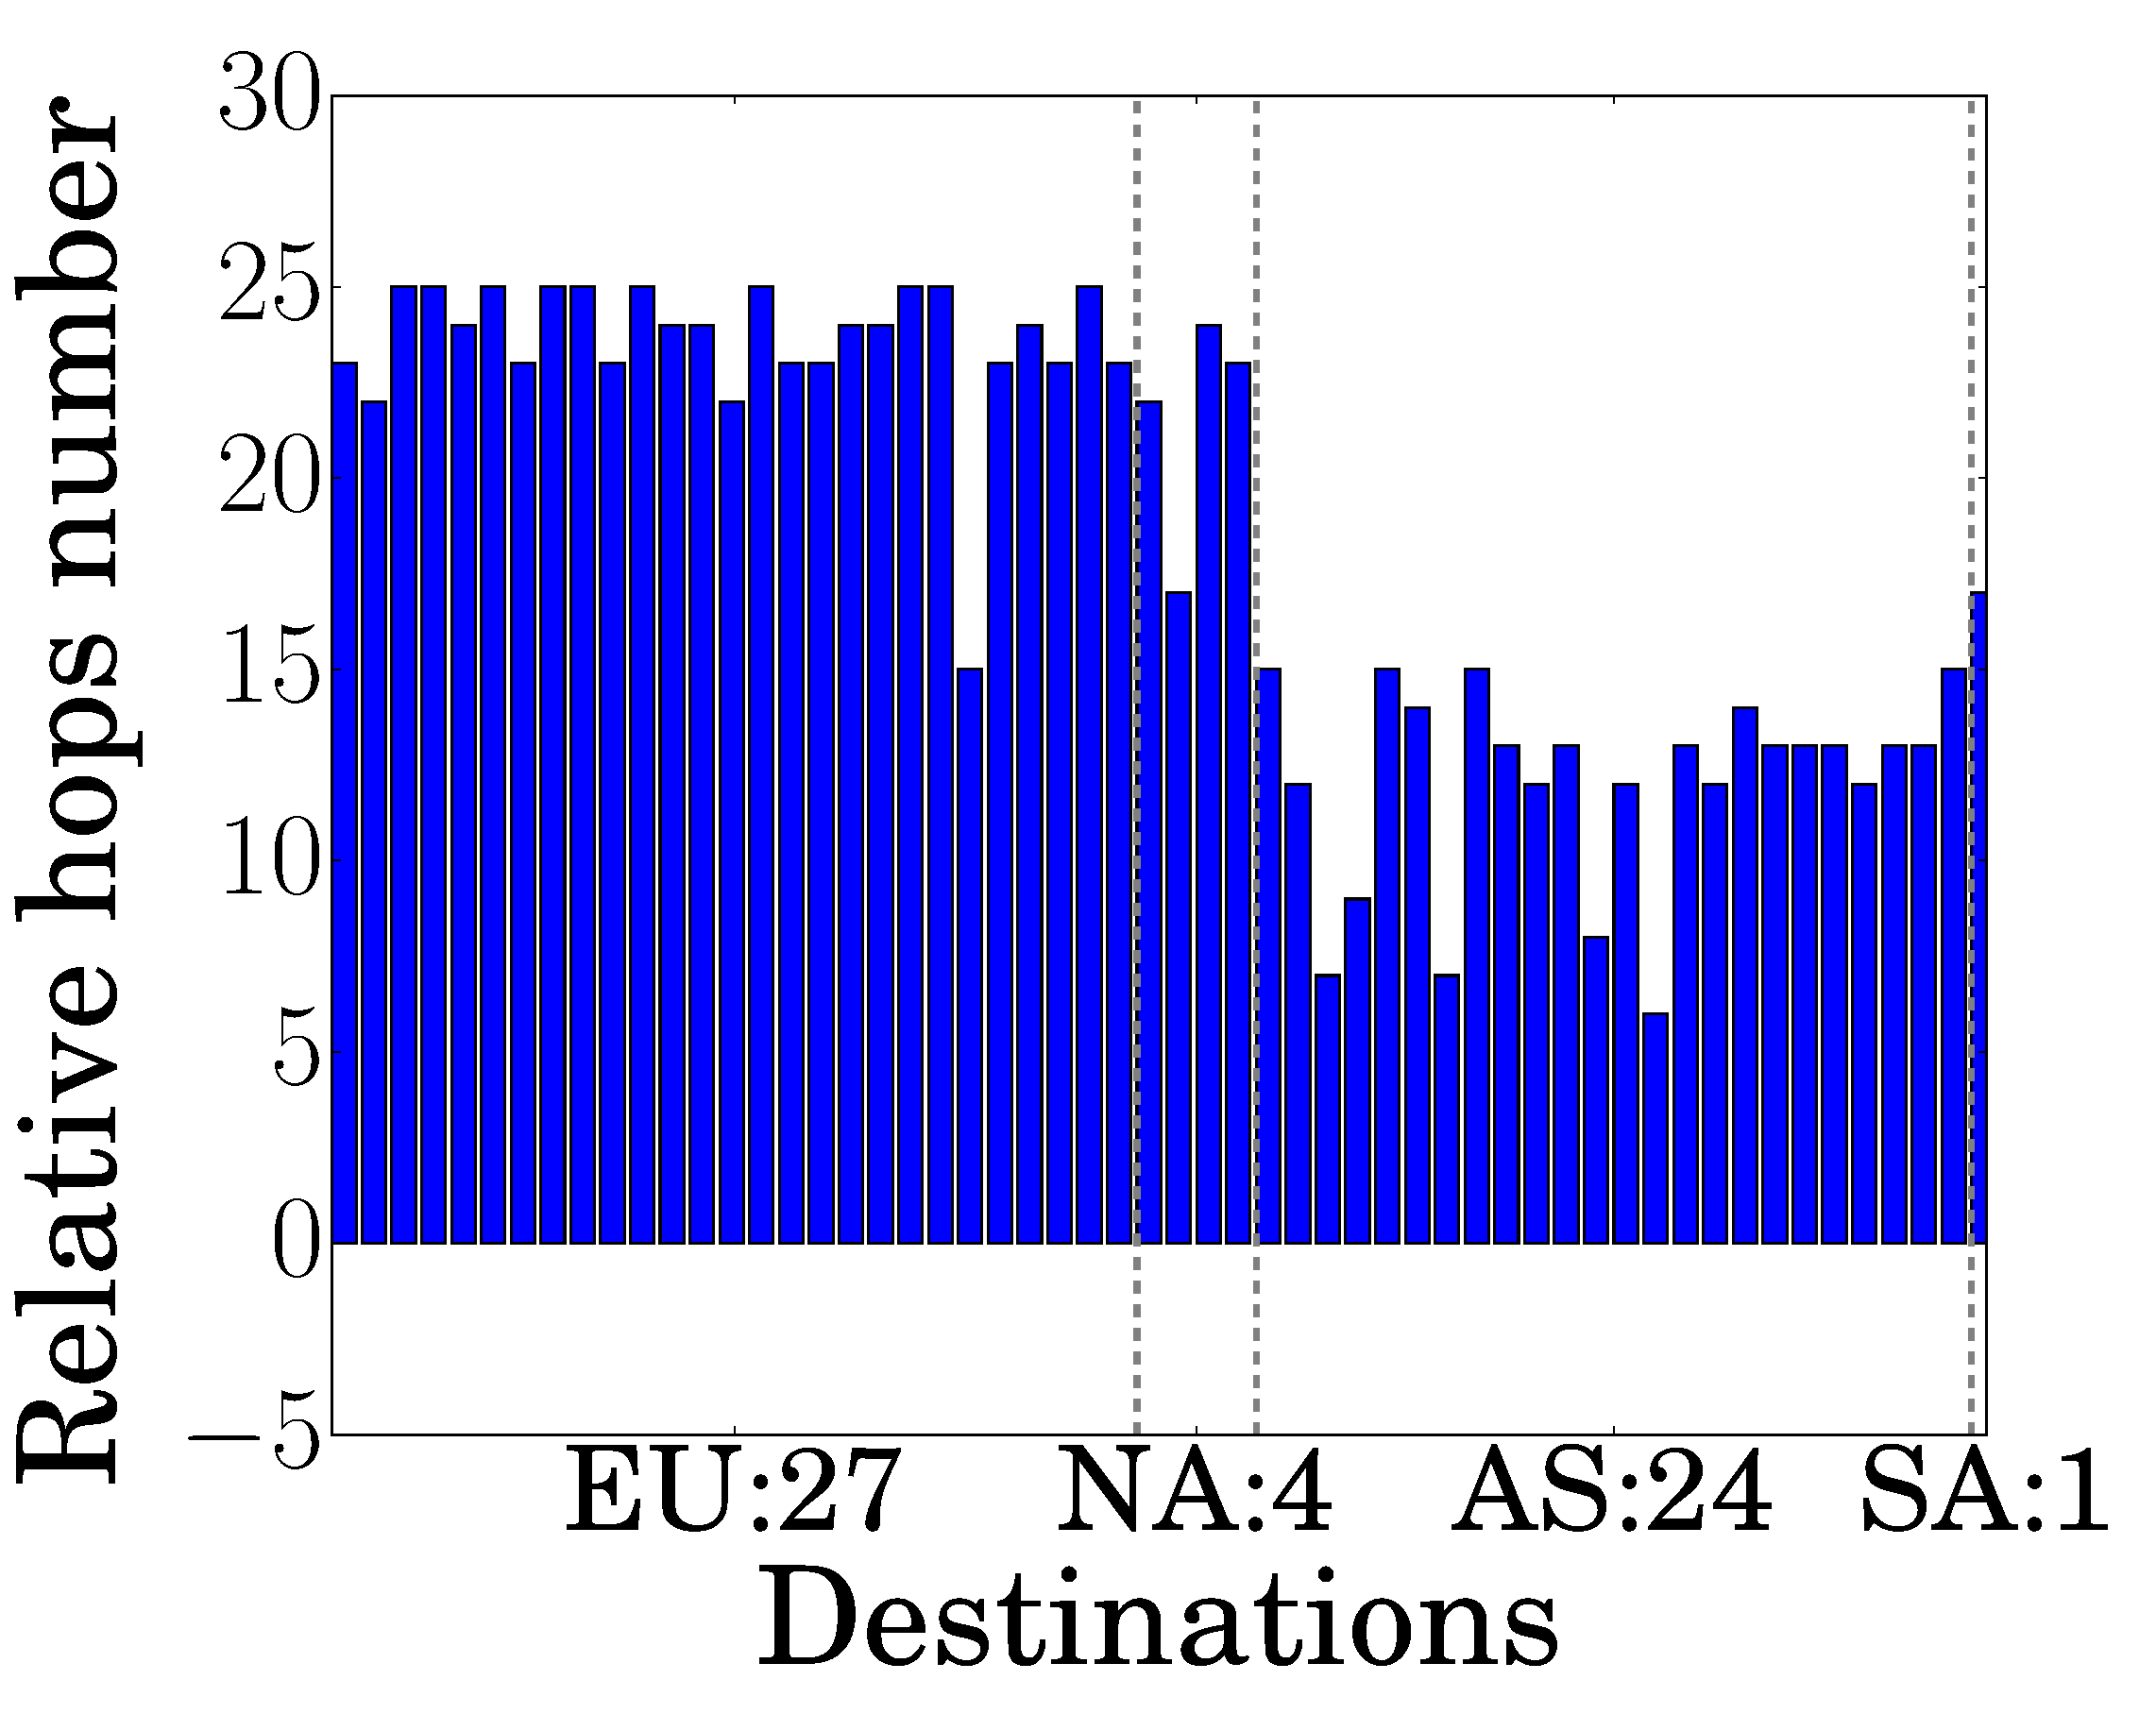
\includegraphics[width=\textwidth]{Pics/v6/Relative_hops_num_LIP6-FranceIX_changed_60.eps}
		\end{center}
	\end{minipage}
	\vspace{-0.5mm}
	\caption{IPv6 Relative hops number clustered by different continents for LISP-Lab (left) and LIP6 (right) from Dataset 2016}
	\label{v6_Relative_hops_num}
\end{figure}
%-< END FIGURE >--------------------------------------------------------------------


%-< SECTION >--------------------------------------------------------------------
%\section{LISP-related Discussion and Conclusion}
\section{Summary}
\label{sec:pxtr_conclusion}
% \begin{itemize}[noitemsep,topsep=0pt]
%     \item PxTR indeed introduces the negative effects for the near destinations, but can be ignored for the intercontinental long-distance transmission.
%     \item Position of PxTR is very important.
%     \item LISP is generally stable, except for the IPv6 performance of LISP Beta Network.
%     \item LISP-Lab PxTR is more reliable than the ones of LISP Beta Network.
%     \item Encapsulating into LISP packets has only 4 hops more compared to the packets being natively forward by xTR.
% \end{itemize}
% In the last years, the Locator/ID Separation Protocol (LISP) has gained attention as promising solutions of several scaling issues the Internet is facing. Various inter-operable implementations, and deployment exist, however, to promote the growth of this relatively novel technology and improve its performance, it requires large scale measurements in real deployments. 
In this chapter, we conduct a six-hours as well as a two-weeks real network measurements with LISP Beta Network, LISP-Lab platform and RIPE Atlas to provide a comprehensive performance evaluation of LISP interworking. Concretely, we provide a first thorough sight on the performance of LISP PxTR. Since the results of experiment in 2016 coincides to the one in 2015 and are more comprehensive. Thus, we conclude this chapter by presenting the observations of the Dataset 2016. 

In our large scale measurement campaign, we take into account 5 probes as sources, 500 IPv4 and 122 IPv6 addresses as destinations, conducting ping and traceroute experiments. We find that the PxTR indeed introduces the negative effects for the destinations located in Europe and America, but the negative impact of PxTR can be ignored for the intercontinental long-distance transmission to Asia destinations. From the experiment, the results show that the position of PxTR is very important. The PxTR either near to the sources or the destinations can decrease the latency a lot. Generally speaking, LISP is stable compared with the reference anchor FranceIX, except for the IPv6 performance of LISP Beta Network. Further, the performance of LISP-Lab PxTR is more reliable than the one of LISP Beta Network, although the latter has 6 worldwide PxTRs used for IPv4 and 2 located in US used for IPv6, whereas LISP-Lab has only 1 PxTR for both IPv4 and IPv6. Compared to leveraging on PxTR, natively forwarding without using LISP decreases the latency, but not much. The traceroute experiment shows that introducing PxTR of course brings more hops, but if the PETR is well configured, so to always have peers to the destinations, there are only 4 more hops compared to the packets being natively forward by xTR without encapsulating with LISP.
